%!TEX root = ../thesis.tex
%*******************************************************************************
%****************************** Fifth Chapter **********************************
%*******************************************************************************
\chapter{Electricity demand prediction}
\label{chapter:demand}
% **************************** Define Graphics Path **************************
\ifpdf
    \graphicspath{{Chapter3/Figs/Raster/}{Chapter3/Figs/PDF/}{Chapter3/Figs/}}
\else
    \graphicspath{{Chapter3/Figs/Vector/}{Chapter3/Figs/}}
\fi


\section{Prologue}

In this Chapter we use several different machine learning and statistical methods to predict electricity demand 30 minutes ahead as well as a day ahead. The 30 minutes ahead methodology is used in the work on day-ahead work. We utilise the errors from the day ahead predictions to see what the impact of such errors are on the day-ahead market. The work looks specifically at the difference in electricity mix with prediction error, as well as carbon emitted. The work on 30-minute ahead forecasting was published in \cite{Kell2018}. 

We introduce this work in Section \ref{forecast:sec:introduction}. Section \ref{forecast:sec:litreview} provides a literature review on the topic of demand forecasting. We introduce the methods used in Section \ref{forecast:sec:methods}. Sections \ref{forecast:sec:shortterm} and \ref{forecast:sec:longterm} look at 30-minute ahead predictions and day-ahead predictions respectively. Section \ref{forecast:sec:longterm} integrates these day ahead projections into the ElecSim model. 

\section{Introduction}
\label{forecast:sec:introduction}

%%%%%%%%%%%%%%%%%%%%%%%%%%%%%%%%%%%%%%%%%%%%%%%%
%%%%%%%%%%%%%%%%%%%%%%%%      Actual Chapter      %%%%%%%%%%%
%%%%%%%%%%%%%%%%%%%%%%%%%%%%%%%%%%%%%%%%%%%%%%%%	


The need for accurate load forecasting is essential for control and planning of electricity generation in electrical grids due to the fact that supply must meet demand \cite{Lu1993}. Short-term electricity demand forecasting has become increasingly important due to the introduction of competitive energy markets. Accurate estimates of demand are required so that the correct amount of electricity is purchased on the wholesale market \cite{Dillon1991}. Electricity is unique to other commodities in that it must be either consumed the moment that it is generated or stored. The difficulties in storing electricity arise from high installation and maintenance costs, inefficiencies and low capacity \cite{Poonpun2008}. It is therefore important to match demand to supply and thus regulate frequency. Failure to accurately forecast electricity demand can lead to financial loss and/or system-wide blackouts \cite{Hines2008}.


The integration of higher proportions of intermittent renewable energy sources (IRES) in the electricity grid will mean that the forecasting of electricity demand will become increasingly important and challenging. Examples of IRES are solar panels and wind turbines, which fluctuate in terms of power output based on localized wind speed and solar irradiance. However, as supply must meet demand at all times and the fact that IRES are less predictable than dispatchable energy sources such as coal and combined-cycle gas turbines (CCGTs) this means extra attention must be made in predicting future demand if we wish to keep, or better reduce, the current frequency of blackouts \cite{Lu1993}. A dispatchable source is one that can be turned on and off by human control and therefore, able to adjust output just in time, at a moment convenient for the grid.



Typically, peaker plants, such as reciprocal gas engines, are used to fill fluctuations in demand that had not been previously planned for. Specifically, peaker plants meet the peaks in demand where other cheaper options are at full capacity. These peaker plants are typically expensive to run and have higher greenhouse gas emissions than their non-peaker counterparts \cite{Mahmood2014}. Whilst peaker plants are also dispatchable plants, not all dispatchable plants are peaker plants. For example coal, which is a dispatchable plant, is run as a base load plant, due to its inability to deal with the fluctuating conditions required of a peaker plant.


To reduce reliance on peaker plants, it is helpful to know how much electricity demand there will be in the future so that more efficient plants can be used to meet this expected demand. This is so that these more efficient plants can be brought up to speed at a time suitable to match the demand. Forecasting a day into the future is especially useful in decentralized electricity markets which have day-ahead markets. Decentralized electricity markets are ones where electricity is provided by multiple generation companies, as opposed to a centralized source, such as a government. To aid in this prediction, machine learning and statistical techniques have been used to accurately predict demand based on several different factors and data sources \cite{Kell2018a}, such as weather \cite{Hong2014}, day of the week \cite{Al-Musaylh2018} and holidays \cite{Vrablecova2017}. 


The introduction of smart meters in many countries (USA, Europe, Canada and South Korea) has led to an influx of high granularity electricity consumption data that can be used for load forecasting \cite{Depuru2011a}. Smart meters are digital devices that measure electricity consumption of individual households at regular intervals (intervals of an hour or less) and offer two-way communication between the meter and utility company. Smart meters aid customers to understand precisely how much electricity they consume at different time intervals, and enable dynamic pricing \cite{Abreu2012a}. Dynamic pricing allows utilities to charge varying prices at different times, for instance, charging a higher price when costly generation sources are used in times of peak demand, and lower prices at night time or weekends when demand is low \cite{Liu2016,Ito2013}. In this Chapter we forecast both 30-minutes ahead using smart meter data, as well as 24-hours ahead to simulate the process made for a day-ahead market. 


%%%%%%%%%%%%%% 30-minute ahead forecasting

Firstly, we explore short term load-forecasting at an interval of 30 minutes ahead and cluster similar users based on their electricity usage. A variety of different forecasting techniques were evaluated such as Random Forests \cite{TinKamHo}, Long-Short Term Memory neural networks (LSTM) \cite{lstm}, Multilayer Perceptron neural networks \cite{book:984557} and \acrfull{svr} \cite{Drucker1997}.

Random Forests are an ensemble based learning method for classification and regression, and are made up of many decision trees. LSTM networks are recurrent neural networks which remember values over arbitrary time intervals. Multilayer Perceptrons are a popular type of neural network which are made up of a minimum of three layers and can be used to make non-linear predictions. \acrshort{svr}s are supervised learning models which analyze data used for regression analysis.

To improve forecasting results, the clustering of smart meter data was evaluated. The technique used for this was \textit{k}-means clustering. An average 24-hour electricity load profile was calculated, and the result used for clustering. The clustered sub-system is then aggregated and separate models trained on this aggregate. The yearly, weekly and daily periodicity of electricity load is accounted for by input variables into the models. Once forecasts for each cluster are made using the individual models, the results are aggregated for the final predictions. These predictions are compared to the actual results and the accuracy measured using mean absolute percentage error (MAPE).






%%%%%%%%%%%%%% Scenario forecasting




Secondly, we introduce day-ahead forecasting and what impact errors have on the long-term dynamics of the market. Various studies have looked at predicting electricity demand at various horizons \cite{Singh2012,Huang2003,Andersen2013}. However, the impact of poor demand predictions on the long-term electricity mix has been studied to a lesser degree.

We compare several machine learning and statistical techniques to predict the energy demand for each hour over the next 24-hour horizon. We chose to predict over the next 24 hours to simulate a day-ahead market, which is often seen in decentralized electricity markets. However, our approach could be utilized for differing time horizons. In addition to this, we use our long-term agent-based model, ElecSim \cite{Kell, Kell2020}, to simulate the impact of different forecasting methods on long-term investments, power plant usage and carbon emissions for the years 2018 through 2035 in the United Kingdom. Our approach, however, is generalizable to any country through parametrization of the ElecSim model.


As part of our work, we utilize online learning methods to improve the accuracy of our predictions. Online learning methods can learn from novel data while maintaining what was learnt from previous data. Online learning is useful for non-stationary datasets, and time-series data where recalculation of a model would take a prohibitive amount of time. Offline learning methods, however, must be retrained every time new data is added. Online approaches are constantly updated and do not require significant pauses while the offline training is being re-run. By training on data that has already been used for training, the computational load and time required increases.

We trial different algorithms and train different models for different times of the year. Specifically, we train different models for the different seasons. We also split weekdays and train both weekends and holidays together. This is due to the fact that holidays and weekend exhibit similar load profiles due to the reduction in industry electricity use and an increase in domestic. This enables a model to become good at a specific subset of the data which share similar patterns, as opposed to having to generalize to all of the data. Examples of the algorithms used are linear regression, lasso regression, random forests, support vector regression, multilayer perceptron neural network, box-cox transformation linear regression and the passive aggressive model. 

We expect a-priori that online algorithms will outperform the offline approach. This is due to the fact that the demand time-series is non-stationary, and thus changes sufficiently over time. In terms of the models, we presume that the machine learning algorithms, such as neural networks, support vector regression and random forests will outperform the statistical methods such as linear regression, lasso regression and box-cox transformation regression. We expect this due to the fact that machine learning has been shown to be able to learn more complex feature representations than statistical methods \cite{Singh2012}. % In addition, our previous work has shown that the random forest was able to outperform neural networks, support vector regression and long short term memory neural networks (LSTM) \cite{Kell2018}. 

However, it should be noted, that such a-priori intuiton, is no substitute for analytical evidence and can (and has) been shown to be wrong in the past, due to imperfect knowledge of the data and understanding of some of the black box models, such as neural networks.

Using online and offline methods, we take the error distributions, or residuals, and fit a variety of distributions to these residuals. We choose the distribution with the lowest sum of squared estimate of errors (SSE). SSE was chosen as the metric to ensure that both positive and negative errors were treated equally, as well as ensuring that large errors were penalized more than smaller errors. We fit over 80 different distributions, which include the Johnson Bounded distribution, the uniform distribution and the gamma distribution. The distribution that best fits the respective residuals is then used and sampled from to adjust the demand in the ElecSim model. We then observe the differences in carbon emissions, and which types of power plants were both invested in and utilized, with each of the different statistical and machine learning methods. To the best of our knowledge, this is the most comprehensive evaluation of online learning techniques to the application of day-ahead load forecasting as well as assessing the impacts of the errors that these models produce on the long-term electricity market dynamics.




%- What are the key take-home messages

We show that online learning has a significant impact on reducing the error for predicting electricity consumption a day ahead when compared to traditional offline learning techniques, such as multilayer artificial neural networks, linear regression, extra trees regression and support vector regression, which are models used in the literature \cite{Lu1993, Ahmad2017, Chen2004}. For a full list of algorithms used in this work see Table \ref{table:hyperparameter-tuning-offline}.

We show that the forecasting algorithm has a non-negligible impact on carbon emissions and use of coal, onshore, photovoltaics, reciprocal gas engines and CCGT. Specifically, the amount of coal, photovoltaics, and reciprocal gas used from 2018 to 2035 was proportional to the median absolute error, while both onshore and offshore wind are inversely proportional to the median absolute error.

Total investments in coal, offshore and photovoltaics are proportional to the median absolute error, while investments in CCGT, onshore and reciprocal gas engines are inversely proportional.


% Contributions of this work


The contributions of this work are:

\begin{enumerate}
	\item A methodology to forecast smart-meter using a \textit{k}-means clustering technique.
	\item The evaluation of different online and offline learning models to forecast the electricity demand profile 24 hours ahead.
	\item Evaluation of poor predictive ability on the long-term electricity market in the UK through the perturbation of demand in the ElecSim simulation.
\end{enumerate}
















\section{Literature review}
\label{forecast:sec:litreview}

In this section we carry out a literature review on 30-minute ahead forecasting, day-ahead forecasting and online forecasting methods. In addition, we cover literature on the impact of forecasting on electricity markets. 

\subsection{30-minute ahead forecasting}

The forecasting of aggregated and clustered electricity demand has been the focus of a considerable amount of research in recent years. The research can generally be classified into two classes, Artificial Intelligence (AI) methods \cite{Kim2000, Tiong2008,Quilumba2014} and classical time series approaches \cite{Huang2003,Nguyen2017}. We trial both approaches in this Chapter.

Singh \textit{et al.} \cite{Singh2012} produced a review of load forecasting techniques and methodologies and reported that hybrid methods, which combine two or more different techniques, are gaining traction, as well as soft computing approaches (AI) such as genetic algorithms. Our work presents a hybrid method which combines \textit{k}-means clustering with multiple different learning algorithms.

\subsubsection{Artificial Intelligence Methods}

Dillon \textit{et al.} presented a neural network for short term load forecasting. Their neural network consisted of three-layers and used adaptive learning for training \cite{Dillon1991}. They proposed the use of weather information to augment their electricity load data. They found better results with the adaptive neural network than with a linear model, or non-adaptive neural network. In contrast to Dillon our work focuses on a non-adaptive neural network and does not take into account weather information.

Chen \textit{et al.} used an \Gls{ANN} to predict electricity demand of three substations in Taiwan. They integrated temperature data and reported that the best results when forecasting residential and commercial substations were during the week due to the influence of weather \cite{Chen1996}. In contrast to the work done by Chen \textit{et al.}, we focus on client-side prediction using smart meter data as opposed to substation data. We were, therefore, able to cluster the data based on load profile, as opposed to geographical location.


\subsubsection{Time Series Methods}

Al-Musaylh \textit{et al.} proposed the use of \acrfull{svr}, an autoregressive integrated moving average (ARIMA) model and a multivariate adaptive regression spline (MARS) in their short term electricity demand forecasting system \cite{Al-Musaylh2018}. They found that for a half, and one-hour forecasting horizons, that the MARS model outperformed both the ARIMA and SVR.

Taylor evaluates different statistical methods including ARIMA, an adaptation of Holt-Winters' exponential smoothing \cite{Holt2004}, and an exponential smoothing method which focuses on the evolution of the intra-day cycle \cite{Taylor2008}. He found that the double seasonal adaptation of the Holt-Winters' exponential smoothing method was the most accurate method for short lead times between 10 and 30 minutes. 

In contrast to Taylor, Fard \textit{et al.} proposed a novel hybrid forecasting method based on both artificial intelligence and classical time series approaches. They utilised the wavelet transform, ARIMA and ANNs for short term load forecasting \cite{Fard2014}. The ARIMA model is created by finding the appropriate order using the Akaike information criterion \cite{Akaike1974}. The ARIMA model models the linear component of the load time series, and the residuals contain the non-linear components. These residuals are then decomposed by the discrete wavelet transform into its sub-frequencies. ANNs are then applied to these sub-frequencies and the outputs of both the ANN and ARIMA models are summed to make the final prediction. They found that this hybrid technique outperformed traditional methods. Our work does not integrate artificial intelligence and classical time series techniques.

\subsubsection{Clustering}

Multiple techniques have been proposed for the clustering of electricity load data prior to forecasting. Both Shu and Luonan, and Nagi \textit{et al.} propose a hybrid approach in which self-organizing maps are used to cluster the data, and Support Vector Regression is used to make predictions \cite{Shu2006,Tiong2008}. This technique proved robust for different data types, and was able to tackle the non-stationarity of the data. Shu showed that this hybrid approach out-performed a single SVR technique, whilst Nagi showed superior results to a traditional ANN system. In contrast to both Nagi \textit{et al.} and Shu and Luonan our work utilises \textit{k}-means as the clustering algorithm 

Quilumba \textit{et al.} also apply machine learning techniques to individual households' electricity consumption by aggregation \cite{Fard2014}. To achieve this aggregation, they use \textit{k}-means clustering to aggregate the households to improve their forecasting ability. The authors also use a neural network based model for forecasting, and show that the number of optimum clusters for forecasting is dependent on the data, with three clusters optimal for a particular dataset, and four for another.

Wijaya \textit{et al.} demonstrated that implementing clusters improved load-forecasting accuracy up to a certain level \cite{Wijaya2010}. Whilst, a study by Ili\'c \textit{et al.} showed that increasing the number of clusters did not improve accuracy \cite{Ilic2013}.

Humeau \textit{et al.} compare MLPs, SVRs and linear regression at predicting smart meter data \cite{Humeau2013}. They aggregate different households and observe which models work the best at each aggregate level. They find that linear regression outperforms both MLP and SVR when forecasting individual households. However, after aggregating over 32 households, SVR outperforms linear regression.


\subsection{Online learning}

Whilst multiple papers have looked at demand-side forecasting \cite{Singh2012}, to the best of our knowledge, the impact of online learning has been discussed with less frequency. In addition to this, our research models the impact of the performance of different algorithms on investments made, electricity sources dispatched and carbon emissions over a 17 year period. To model this, we use the long-term electricity market agent-based model, ElecSim. In our work, we trial a different set of algorithms to our problem. Due to time and compute constraints, we do not trial the additional techniques discussed in this literature review within our work. 

Johansson \textit{et al}. apply online machine learning algorithms for heat demand forecasting \cite{Johansson2017}. They find that their demand predictions display robust behaviour within acceptable error margins. They find that artificial neural networks (ANNs) provide the best forecasting ability of the standard algorithms and can handle data outside of the training set. Johansson \textit{et al.}, however, do not look at the long-term effects of different algorithms on their application.

Baram \textit{et al}. combine an ensemble of active learners by developing an active-learning master algorithm \cite{Baram2003}. To achieve this, they propose a simple maximum entropy criterion that provides effective estimates in realistic settings. Their active-learning master algorithm is empirically shown to, in some cases, outperform the best algorithm in the ensemble on a range of classification problems.

Schmitt \textit{et al}. also extends on existing algorithms through an extension of the FLORA algorithm in \cite{Schmitt2008, Widmer1996}. The FLORA algorithm generates a rule-based model, which has the ability to make binary decisions. Their FLORA-MC enhances the FLORA algorithm for multi-classification and numerical input values. They use this algorithm for an ambient computing application. Ambient computing is where computing and communication merges into everyday life. They find that their model outperforms traditional offline learners by orders of magnitude.

Similarly to us, Pindoriya \textit{et al}. trial several different machine learning methods such as adaptive wavelet neural network (AWNN). They find that AWNN has good prediction properties when compared to other forecasting techniques such as wavelet-ARIMA, multilayer perceptron (MLP) and radial basis function (RBF) neural networks as well as the fuzzy neural network (FNN).


Goncalves Da Silva \textit{et al}. show the effect of prediction accuracy on local electricity markets \cite{GoncalvesDaSilva2014}. To this end, they compare forecasting of groups of consumers in comparison to single individuals. They trial the use of the Seasonal-Naïve and Holt-Winters algorithms and look at the effect that the errors have on trading in an intra-day electricity market of consumers and prosumers. They found that with a photovoltaic penetration of 50\%, over 10\% of the total generation capacity was uncapitalized and roughly 10, 25 and 28\% of the total traded volume were unnecessary buys, demand imbalances and unnecessary sells respectively. This represents energy that the participant has no control. Uncapitalized generation capacity is where a participant could have produced energy, however, it was not sold on the market. Additionally, due to forecast errors, the participant might have sold less than it should have. Our work, however, focuses on a national electricity market, as opposed to a local market.




\section{Methods}
\label{forecast:sec:methods}

In this section, we explore the principles behind the methods used in this Chapter. 


%%%%%%%%%%%%%%%%%%%%%%%%%%%%%%%%%%%%%%%%%%%%%%%%
%%%%%%%%%%%%%%%%%%%%%%%%      Paper 1    %%%%%%%%%%%%%%%%
%%%%%%%%%%%%%%%%%%%%%%%%%%%%%%%%%%%%%%%%%%%%%%%%	


%\subsection{Decision Tree}
%
%A decision tree is a statistical model used for either classification or regression \cite{breiman1984classification}. Load forecasting is a regression problem, and therefore regression trees are used in this paper. 
%
%Decision trees recursively partition data into nodes with different labels until the termination criteria is met. This is typically initiated when it is not possible to have children nodes with different output labels. The terminal nodes are known as leaves and they represent the different outputs.
%
%\subsection{Random Forest}
%
%A Random Forest is an ensemble method that combines the predictions of many decision trees \cite{Breiman2001}. Each decision tree is fit by a random sample, with replacement, of the training data. The final decision of the Random Forest is decided by a majority case wins vote on each of the decision trees.

\subsection{Error Metrics}

\subsubsection{Mean Absolute Percentage Error}

The mean absolute percentage error (MAPE) is a measure of prediction accuracy which is used in this thesis. It can be defined as follows:

\begin{equation}
MAPE=\frac{1}{n}\sum_{i=1}^n\left|\frac{y_i-\hat{y}_i}{y_i}\right|\times 100\%
\end{equation}

\noindent where $y_i$ is the actual value, $\hat{y}_i$ is the forecast value and $n$ is the number of points forecast \cite{Li2016}.

\subsubsection{Root Mean Squared Error}

The root mean squared error (RMSE) is a measure between the values predicted by a model and the observed values. The RMSE is the sample standard deviation of the differences between the predicted and observed values.

The RMSE is defined as follows:
\begin{equation}
RMSE = \sqrt[]{\frac{\sum_{t=1}^n(\hat{y}_i-y_i)^2)}{n}}
\end{equation}

\noindent where $\hat{y}_i$ are the predicted values, $y_i$ are the observed values, and $n$ is the number of observations.


\subsubsection{Mean Absolute Scaled Error}

The mean absolute scaled error (MASE) is a measure of accuracy of forecasts. It is defined as the mean absolute error of the forecast values, divided by the mean absolute error of the in-sample one-step naive forecast. MASE can be scaled across difference scales, has symmetry for both positive and negative errors, is interpretable and has predictable behaviour for a value of 0. 

MASE can be defined as follows:

\begin{equation}
MASE = mean\left(\frac{|e_j|}{\frac{1}{T-1}\sum_{t=2}^T|Y_t-Y_{t-1}|}\right)=\frac{\frac{1}{J}\sum_j|e_j|}{\frac{1}{T-1}\sum_{t=2}^{T}|Y_t-Y_{t-1}|}
\end{equation}

\noindent where $e_j$ is the forecast error for a given period, $J$ is the number of forecasts. Where $e_j$ is defined as the actual value ($Y_j$) minus the forecast value ($F_j$) for that period. The denominator is the mean absolute error of the one-step naive forecast method on the training set. This naive forecast is the actual value from the prior period, or $F_t=Y_{t-1}$. $T$ is the total number of forecasts.




















%%%%%%%%%%%%%%%%%%%%%%%%%%%%%%%%%%%%%%%%%%%%%%%%
%%%%%%%%%%%%%%%%%%%%%%%%      Paper 2    %%%%%%%%%%%%%%%%
%%%%%%%%%%%%%%%%%%%%%%%%%%%%%%%%%%%%%%%%%%%%%%%%	












\subsection{Machine learning}

Machine learning is a methodology for finding and describing structural patterns in data \cite{Witten2011}. Offline learning models are trained with the data availalable at a single point in time. With non-stationary data where underlying distributions change, the model must be retrained at periodic intervals, determined by how quickly the model goes out of step with the true data. With online learning, the model is able to retrain every time a new data point becomes available, without having to retrain the entire model. This makes these models good for time-series data which exhibit moderate to significant non-stationary properties, such as electricity demand profiles.





\subsection{Online learning}

%Online machine learning is a type of machine learning algorithm that can be used on dynamic datasets, such as time-series data. In traditional machine learning algorithms, when new data is obtained, the historical and new data must be used to retrain the entire model with a new model. This can be costly both in terms of time and in computation power \cite{Li2016}. Online algorithms, therefore, avoids the repeated retraining of data and improves the learning efficiency \cite{Rong2009}. Online training can also adapt to situations where the underlying system you are predicting on is changing over time, or non-stationary.



Examples of online learning algorithms are Passive Aggressive (PA) Regressor \cite{Gzik2014}, Linear Regression, Box-Cox Regressor \cite{Box1964}, K-Neighbors Regressor \cite{forgy65} and Multilayer perceptron regressor \cite{Hinton1989}. For our work, we trial the stated algorithms, in addition to a host of offline learning techniques. The offline techniques trialled were Lasso regression \cite{Tibshirani1996a}, ridge regression \cite{GeladiPaul1994Mrac},  Elastic Net \cite{Geostatistics2010}, Least Angle Regression \cite{Fike1988}, Extra Trees Regressor \cite{Fike1988}, Random Forest Regressor \cite{Breiman2001}, AdaBoost Regressor \cite{Freund1997}, Gradient Boosting Regressor \cite{316} and Support vector regression \cite{Cortes1995}. We chose the boosting and random forest techniques due to our previous successes of these algorithms when applied to electricity demand forecasting \cite{Kell2018}. We trialled the additional algorithms due to availability of these algorithms using the scikit-learn package and online learning package, Creme \cite{scikit-learn,creme}. %, and online versions of Multilayer perceptron regressor, K-Neighbors regressor, linear regression.

%We trial the previously mentioned statistical and machine learning algorithms and vary the parameters using grid search and cross-validation using scikit-learn \cite{scikit-learn}.

\subsection{Linear regression models}


Linear regression is a linear approach to modelling the relationship between a dependent variable and one or more independent variables. Linear regressions can be used for both online and offline learning. In this work, we used them for both online and offline learning. Linear regression models are often fitted using the least squares approach. The least squares approach minimizes the sum of the squares of the residuals. 

Other methods for fitting linear regressions are by minimizing a penalized version of the least squares cost function, such as in ridge and lasso regression \cite{Tibshirani1996a, GeladiPaul1994Mrac}. Ridge regression is a useful approach for mitigating the problem of multicollinearity in linear regression. Multicollinearity is where one predictor variable can be linearly predicted from the others with a high degree of accuracy. This phenomenon often occurs in models with a large number of parameters. 

In ridge regression, the OLS loss function is augmented so that we not only minimize the sum of squared residuals but also penalized the size of parameter estimates, in order to shrink them towards zero:
\begin{equation}
L_{ridge}(\hat{\beta})=\sum^n_{i=1}(y_i-x'_i\hat{\beta})^2+\lambda\sum^m_{j=1}\hat{\beta^2_j}=||y-X\hat{\beta}||^2+\lambda||\hat{\beta}||^2.
\end{equation}

Where $\lambda$ is the regularization penalty which can be chosen through cross-validation, or the value that minimizes the cross-validated sum of squared residuals, for instance. $n$ is the number of observations of the response variable, $Y$, with a linear combination of $m$ predictor variables, $X$, and we solve for $\hat{\beta}$, where $\hat{\beta}$ are the OLS parameter estimates.



Lasso is a linear regression technique which performs both variable selection and regularization. It is a type of regression that uses shrinkage. Shrinkage is where data values are shrunk towards a central point, such as the mean. The lasso model encourages models with fewer parameters. This enables the selection of models with fewer numbers of parameters, or automate the process of variable selection.

Under Lasso the loss is defined as:

\begin{equation}
L_{lasso}(\hat{\beta})=\sum^n_{i=1}(y_i-x'_i\hat{\beta})^2+\lambda\sum^m_{j=1}|\hat{\beta}_j|.
\end{equation}

The only difference between lasso and ridge regression is the penalty term.

Elastic net is a regularization regression that linearly combines the penalties of the lasso and ridge methods. Specifically, Elastic Net aims to minimize the following loss function:
\begin{equation}
L_{enet}(\hat{\beta})=\frac{\sum^n_{i=1}(y_i-x'_i\hat{\beta})^2}{2n}+\lambda(\frac{1-\alpha}{2}\sum^m_{j=1}\hat{\beta}^2_j+\alpha\sum^m_{j=1}|\hat{\beta_j}|),
\end{equation}
where $\alpha$ is the mixing parameter between ridge ($\alpha=0$) and lasso ($\alpha=1$). The two parameters $\lambda$ and $\alpha$ can be tuned.


Least Angle Regression (LARS) provides a mean of producing an estimate of which variables to include in a linear regression, as well as their coefficients.


%\subsubsection{Boosting methods}
%
%%AdaBoost Regressor, Gradient Boosting Regressor



\subsection{Decision tree-based algorithms}

The decision tree is a model which goes from observations to output using simple decision rules inferred from data features \cite{Quinlan}. To build a regression tree, recursive binary splitting is used on the training data. Recursive binary splitting is a greedy top-down algorithm used to minimize the residual sum of squares. The RSS, in the case of a partitioned feature space with $M$ partitions, is given by:

\begin{equation}
RSS=\sum^M_{m=1}\sum_{i\in R_m}(y-\hat{y}_{R_m})^2.
\end{equation}

\noindent Where $y$ is the value to be predicted, $\hat{y}$ is the predicted value for partition $R_m$.



Beginning at the top of the tree, a split is made into two branches. This split is carried out multiple times and the split is chosen that minimizes the current RSS. To obtain the best sequence of subtrees cost complexity, pruning is used as a function of $\alpha$. $\alpha$ is a tuning parameter that balances the depth of the tree and the fit to the training data. This parameter can be tuned using cross-validation.


The AdaBoost training process selects only the features of a model known to improve the predictive power of the model \cite{Freund1997}. By doing this, the dimensionality of the model is reduced and can improve compute time. This can be used in conjunction with multiple different models. In our work, we utilized the decision tree based algorithm with AdaBoost.


Random Forests are an ensemble learning method for classification and regression \cite{Breiman2001}. Ensemble learning methods use multiple learning algorithms to obtain better predictive performance. They work by constructing multiple decision trees at training time, and outputting the predicted value that is the mode of the predictions of the individual trees.

To ensure that the individual decision trees within a Random Forest are not correlated, bagging is used to sample from the data. Bagging is the process of randomly sampling with replacement of the training set and fitting the trees. This has the benefit of reducing the variance of the model without increasing the bias. 

Random Forests differ in one way from this bagging procedure. Namely, using a modified tree learning algorithm that selects, at each candidate split in the learning process, a random subset of the features, known as feature bagging. Feature bagging is undertaken due to the fact that some predictors with a high predictive ability may be selected many times by the individual trees, leading to a highly correlated Random Forest.

ExtraTrees adds one further step of randomization \cite{Fike1988}. ExtraTrees stands for extremely randomized trees. There are two main differences between ExtraTrees and Random Forests. Namely, each tree is trained using the whole learning sample (And not a bootstrap sample), and the top-down splitting in the tree learner is randomized. That is, instead of computing an optimal cut-point for each feature, a random cut-point is selected from a uniform distribution. The split that yields the highest score is then chosen to split the node. 


\subsection{Gradient Boosting}

Gradient boosting is also an ensemble model \cite{316}. Gradient boosting optimizes a cost-function over function space by iteratively choosing a function that points in the negative gradient descent direction, known as a gradient descent method.

\subsection{Support vector regression}





%%%%%%%%%%%%%%%%%%%%%%%%%%%%%%%%%%%%%%%%%%%%%%%%
%%%%%%%%%%%%%%%%%%%%%%%%      Paper 1    %%%%%%%%%%%%%%%%
%%%%%%%%%%%%%%%%%%%%%%%%%%%%%%%%%%%%%%%%%%%%%%%%	


%A Support Vector Regression model maps input data, $x$, into a higher-dimensional feature space non-linearly. Given the input data:
%
%\begin{equation}
%(x_1,y_1), \ldots,(x_i,y_i),\ldots,(x_n,y_n) 
%\end{equation}
%
%\noindent where $x_i$ is the input, and $y_i$ is the output value of $x_i$. Support Vector Regression solves an optimization problem \cite{Shu2006,Chen2004}
%
%\begin{equation}
%\min_{\omega,b,\xi,\xi^{*}}\frac{1}{2}\omega^T\omega+C\sum_{i=1}^{n}(\xi_i+\xi_i^*)
%\end{equation}
%
%\noindent subject to
%\begin{align}
%\begin{multlined}
%\label{svr:constrains}
%y_i-(\omega^T\phi(x_i)+b)\leq\varepsilon+\xi_i^{*},\\
%(\omega^T\phi(x_i)+b)-y_i\leq\varepsilon+\xi_i,\\
%\xi_i,\xi^*_i\geq0,i=1,\ldots,n
%\end{multlined}
%\end{align}
%
%
%\noindent $x_i$ is mapped to a higher dimensional space using the function $\phi$. The $\varepsilon$-insensitive tube $(\omega^T\phi(x_i)+b)-y_i\leq\varepsilon$ is a range shown in Figure \ref{fig:insensitive} in which errors are permitted. $\xi_i$ and $\xi^*_i$ are slack variables which allow errors for data points which fall outside of $\varepsilon$. This enables the optimisation to take into account the fact that data does not always fall within the $\varepsilon$ range \cite{Smola2004}.
%
%The constant $C>0$ determines the trade-off between the flatness of the support vector function. $\omega$ is the model fit by the SVR. The parameters which control regression quality are the cost of error $C$, the width of the tube $\varepsilon$, and the mapping function $\phi$ \cite{Shu2006,Chen2004}. 
%
%Figure \ref{fig:insensitive} demonstrates this principle, where only data points which fall outside of the $\varepsilon$-insensitive tube are penalised in the cost function
%
%\begin{figure}[b]
%	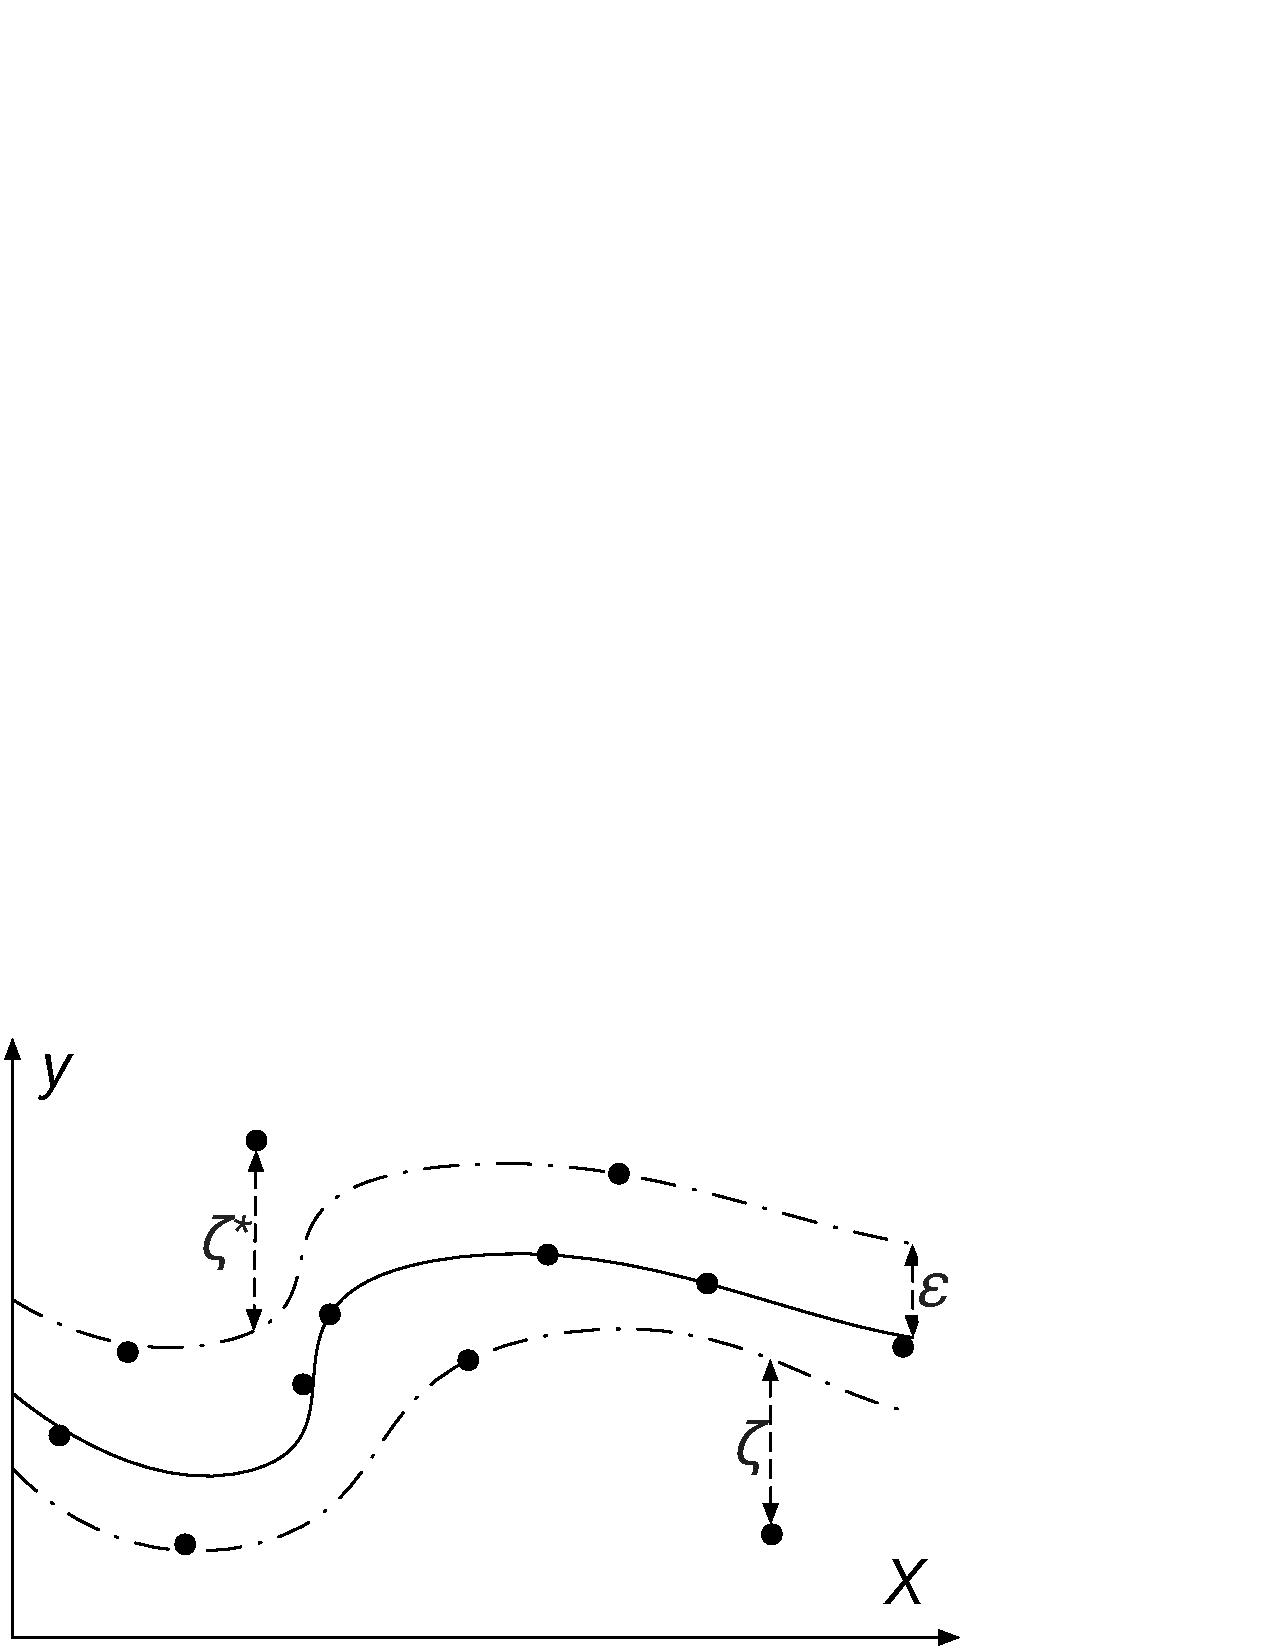
\includegraphics[width=0.8\textwidth]{Chapter5/figures/short-term-forecasting/Kell_eEnergy_Fig2.pdf}
%	\caption{$\varepsilon$-insensitive band for SVR \cite{Shu2006}.}
%	\label{fig:insensitive}
%\end{figure}
%
%The constraints shown in \eqref{svr:constrains} imply that most of the data $x_i$ falls within the tube $\varepsilon$. By minimizing the training error $C\sum_{i=1}^n(\xi_i+\xi_i^*)$, and the regularisation term $\frac{1}{2}\omega^T\omega$, under-fitting and over-fitting are avoided. 
%
%Due to the fact that $\phi$ maps $x_i$ to a high or infinite dimensional space, $\omega$ can be solved, subject to the constraints in \eqref{svr:constrains}, by Lagrangian optimisation. Thus the dual problem is solved \cite{Shu2006,Chen2004,Smola2004}:
%
%\begin{align}
%\min_{\alpha\alpha^*}\frac{1}{2}(\alpha-\alpha^*)^TQ(\alpha-\alpha^*)+\varepsilon\sum^n_{i=1}(\alpha_i+\alpha_i^*)+\sum_{i=1}^ny_i(\alpha_i-\alpha_i^*)
%\end{align}
%
%\noindent subject to 
%\begin{align}
%\begin{multlined}
%\sum_{i=1}^n(\alpha_i-\alpha_i^*)=0,\\
%0\leq\alpha_i,\alpha^*_i\leq C,i=1,\ldots,n
%\end{multlined}
%\end{align}
%
%\noindent where $Q_{ij}=\phi(x_i)^T\phi(x_j)$, $a_i$ and $a_i^*$ are Lagrange multipliers. However due to the large number of elements in $\phi(x)$ we apply a "kernel trick" to do the mapping implicitly. Now, the optimisation can be calculated using solely dot products. An example of the linear function kernel is listed below, which is used in this paper:
%\begin{equation}
%K(x,y)=x^Ty.
%\end{equation}
%
%








%%%%%%%%%%%%%%%%%%%%%%%%%%%%%%%%%%%%%%%%%%%%%%%%
%%%%%%%%%%%%%%%%%%%%%%%%      Paper 2    %%%%%%%%%%%%%%%%
%%%%%%%%%%%%%%%%%%%%%%%%%%%%%%%%%%%%%%%%%%%%%%%%	



Support vector regression is an algorithm which finds a hyperplane and decision boundary to map an input domain to an output \cite{Cortes1995}. The hyperplane is chosen by minimizing the error within a certain tolerance.

Suppose we have the training set: $(x_1,y_1), \ldots,(x_i,y_i),\ldots,(x_n,y_n)$, where $x_i$ is the input, and $y_i$ is the output value of $x_i$. Support Vector Regression solves an optimization problem \cite{Shu2006,Chen2004}, under given parameters $C>0$ and $\varepsilon >0$, the form of support vector regression is \cite{Drucker1997}: 

\begin{equation}
\min_{\omega,b,\xi,\xi^{*}}\frac{1}{2}\omega^T\omega+C\sum_{i=1}^{n}(\xi_i+\xi_i^*)
\end{equation}

\noindent subject to
\begin{align}
\begin{multlined}
\label{svr:constrains}
y_i-(\omega^T\phi(x_i)+b)\leq\varepsilon+\xi_i^{*},\\
(\omega^T\phi(x_i)+b)-y_i\leq\varepsilon+\xi_i,\\
\xi_i,\xi^*_i\geq0,i=1,\ldots,n
\end{multlined}
\end{align}

\noindent $x_i$ is mapped to a higher dimensional space using the function $\phi$. The $\varepsilon$-insensitive tube $(\omega^T\phi(x_i)+b)-y_i\leq\varepsilon$ is a range in which errors are permitted. $\xi_i$ and $\xi^*_i$ are slack variables which allow errors for data points which fall outside of $\varepsilon$. This enables the optimization to take into account the fact that data does not always fall within the $\varepsilon$ range \cite{Smola2004}.

The constant $C>0$ determines the trade-off between the flatness of the support vector function. $\omega$ is the model fit by the SVR. The parameters which control regression quality are the cost of error $C$, the width of the tube $\varepsilon$, and the mapping function $\phi$ \cite{Shu2006,Chen2004}. 


\subsection{K-Neighbors Regressor}

K-Neighbors regression is a non-parametric method used for regression \cite{forgy65}. The input consists of a new data point, and the algorithm finds the \textit{k} closest training examples in the feature space. The output is the average value of the \textit{k} nearest neighbours.



%\subsection{Multilayer perceptron}




%%%%%%%%%%%%%%%%%%%%%%%%%%%%%%%%%%%%%%%%%%%%%%%%
%%%%%%%%%%%%%%%%%%%%%%%%      Paper 1    %%%%%%%%%%%%%%%%
%%%%%%%%%%%%%%%%%%%%%%%%%%%%%%%%%%%%%%%%%%%%%%%%	


%\subsection{Artificial Neural Network}
%
%
%\begin{figure}
%	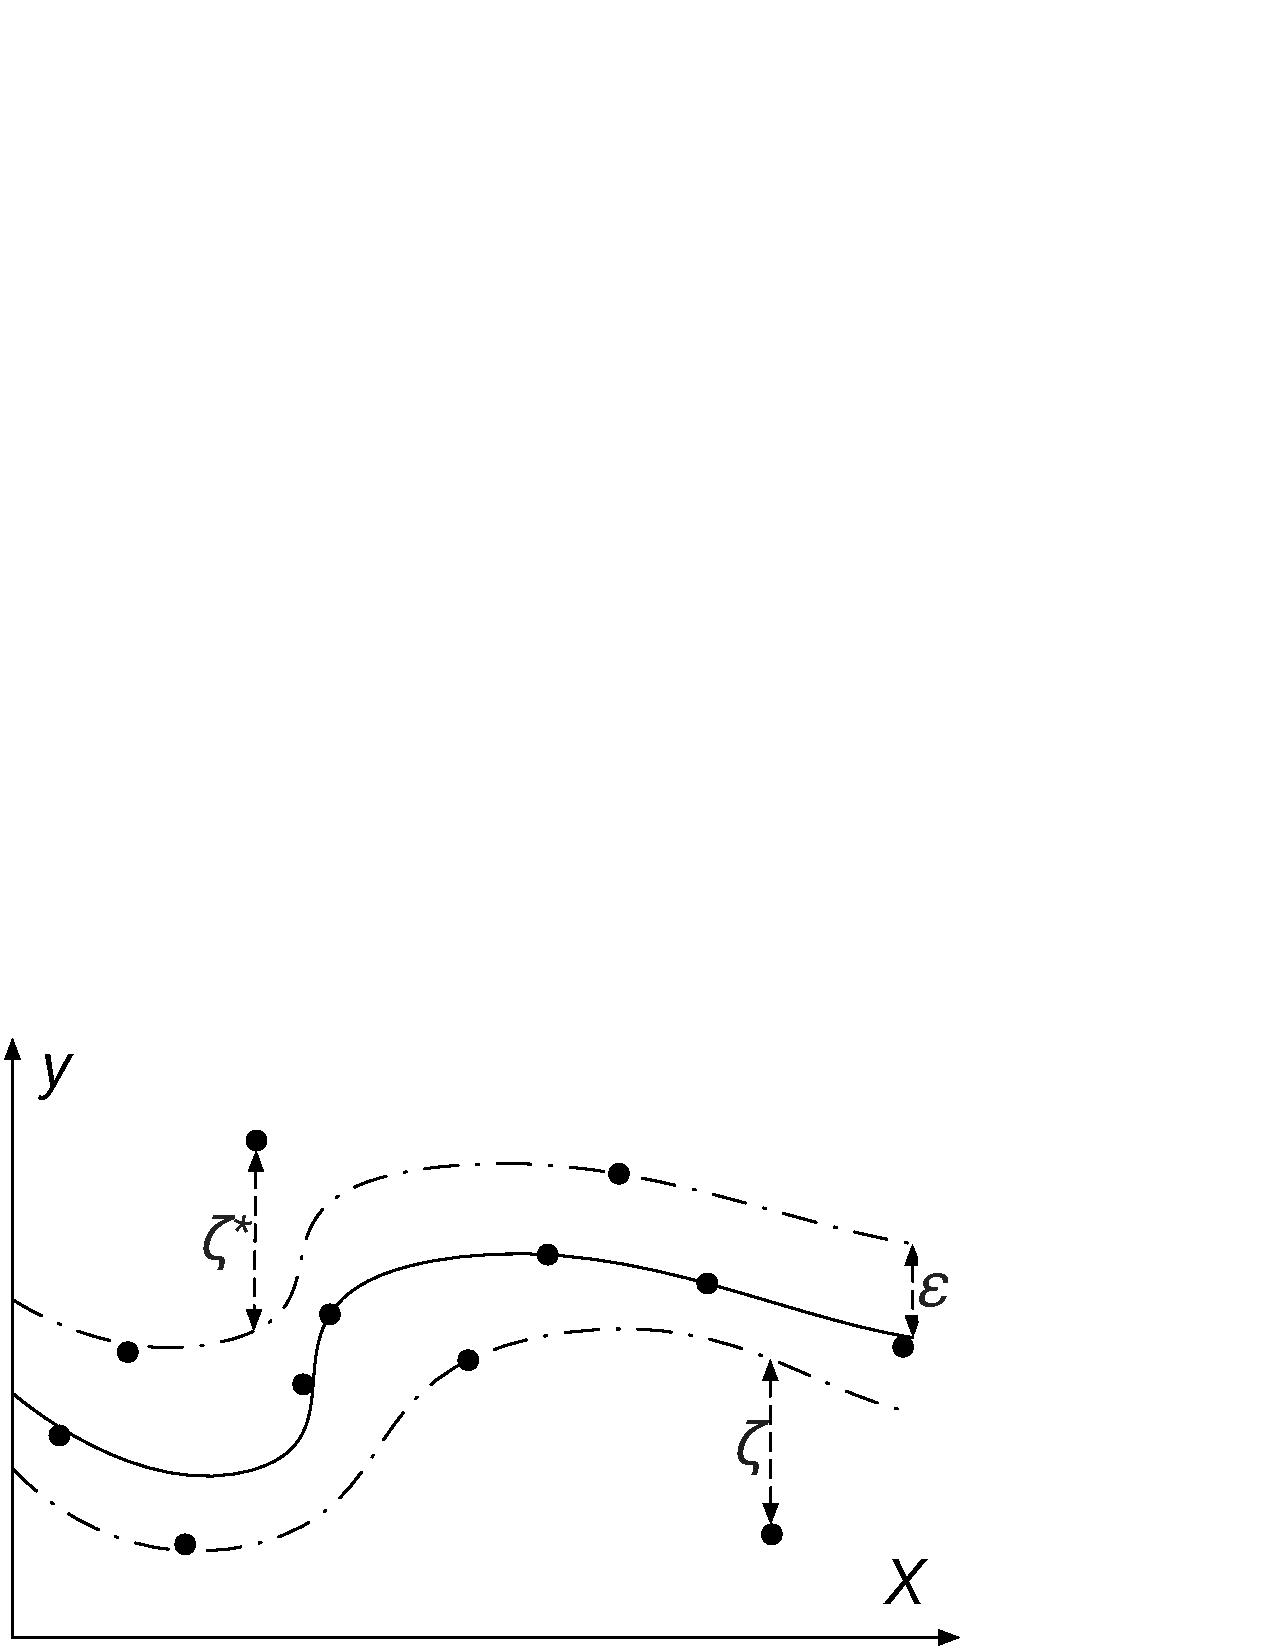
\includegraphics[width=0.8\textwidth]{Chapter5/figures/short-term-forecasting/Kell_eEnergy_Fig2.pdf}
%	\caption{A three layer feed forward neural network.}
%	\label{fig:mlp}
%\end{figure}
%
%
%Artificial Neural Networks are a type of model which allow for non-linear relationships to be modeled between the input and output data \cite{Akaike1974}. A popular neural network is a feed forward multilayer network. Fig. \ref{fig:mlp} shows a three layer feed forward neural network with a single output unit, \textit{k} hidden units, $n$ input units. $w_{ij}$ is the connection weight from the $i$th input unit to the $j$th hidden unit,  and $T_j$ is the connecting weight from the $j$th hidden unit to the output unit \cite{Pao2007}. These weights transform the input variables in the first layer to the output variable in the final layer based upon the training data. 
%
%Typically, a dataset is split into three sections, the test set, training set and validation set. The training set is used to find the connection weights of the network, whilst the test set is used to determine the accuracy of the models. The validation set allows for an unbiased evaluation of the model whilst tuning the hyperparameters, and can avoid overfitting by stopping training if the error begins to increase.
%
%For a univariate time series forecasting problem, suppose we have N observations $y_1, y_2, \ldots, y_N$ in the training set, 
%\begin{equation}
%y_{N+1}, y_{N+2}, \ldots, y_{N+m}
%\end{equation}
%\noindent in the test set and we are required to predict \textit{m} periods ahead \cite{Pao2007}. 
%
%The training patterns are as follows:
%\begin{align}
%y_{p+m} & =f(y_p, y_{p-1},\ldots,y_1)\\
%y_{p+m+1} & =f(y_{p+1}, y_{p},\ldots,y_2)\\
%&\vdotswithin  \notag \\
%y_{N} & =f(y_{N-m},y_{N-m-1},\ldots,y_{N-m-p+1})
%\end{align}
%
%\noindent where $f$ is the function made up of weights and activation functions in the trained neural network.
%
%The $m$ testing patterns are 
%
%\begin{align}
%y_{N+1} & =f(y_{N+1-m}, y_{N-m},\ldots,y_{N-m-p+2})\\
%y_{N+2} & =f(y_{N+2-m}, y_{N-m+1},\ldots,y_{N-m-p+3})\\
%&\vdotswithin  \notag \\
%y_{N+m} & =f(y_{N},y_{N-1},\ldots,y_{N-p+1})
%\end{align}
%
%The training objective is to minimize the overall predictive error means (SSE) by adjusting the connection weights. For this network structure the SSE can be written as:
%\begin{equation}
%SSE = \sum_{i=p+m}^N(y_i-\hat{y}_i)
%\end{equation}
%
%\noindent where $\hat{y}_i$ is the output from the network. The number of input nodes corresponds to the number of lagged observations. Having too few or too many input nodes can affect the predictive ability of the neural network \cite{Pao2007}.







%%%%%%%%%%%%%%%%%%%%%%%%%%%%%%%%%%%%%%%%%%%%%%%%
%%%%%%%%%%%%%%%%%%%%%%%%      Paper 2    %%%%%%%%%%%%%%%%
%%%%%%%%%%%%%%%%%%%%%%%%%%%%%%%%%%%%%%%%%%%%%%%%	








\begin{figure}
	\centering
	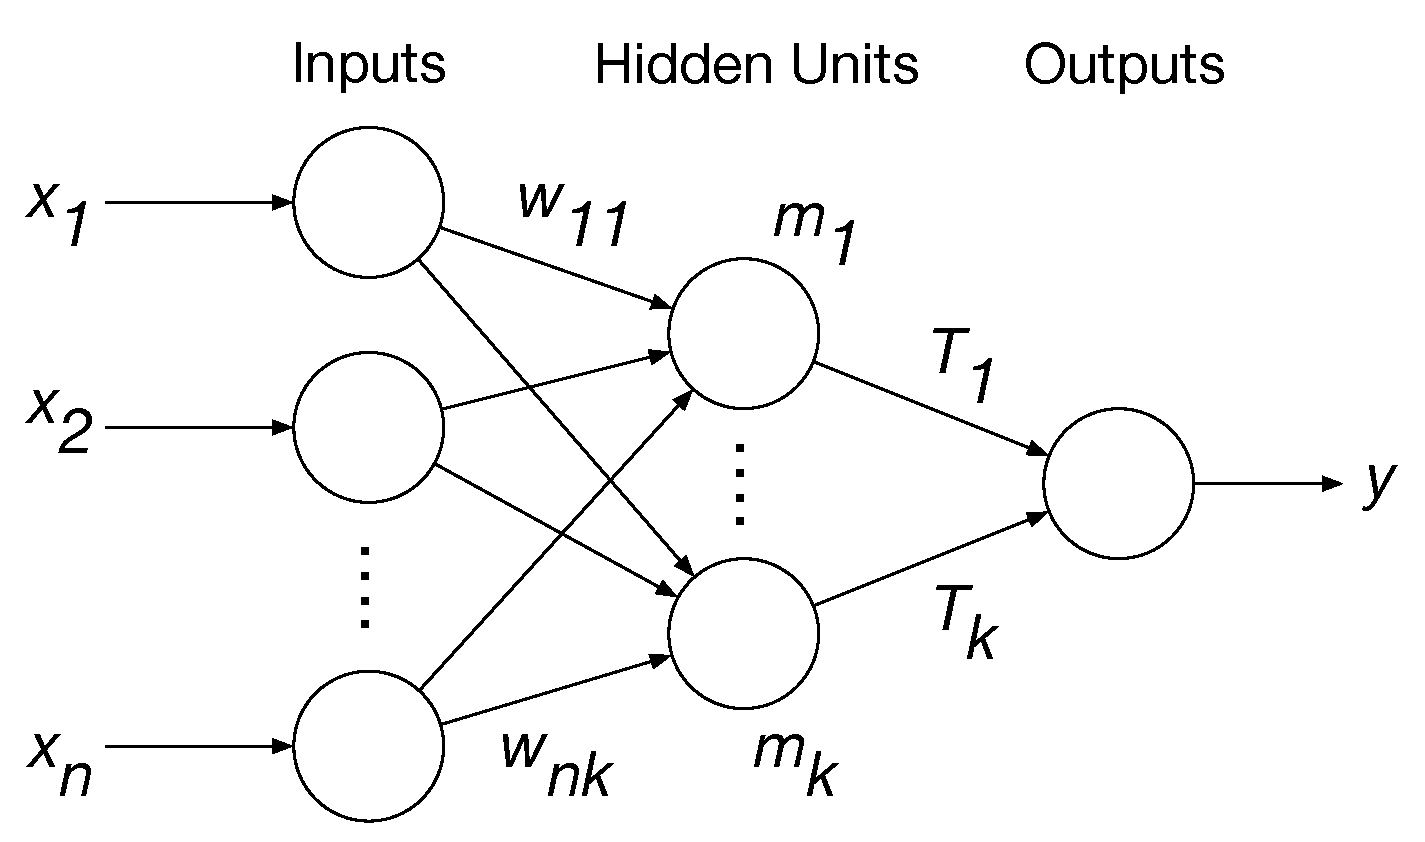
\includegraphics[width=0.4\textwidth]{Chapter5/figures/market-forecasting/methods/Kell_eEnergy_Fig1.eps}
	\caption{A three-layer feed forward neural network.}
	\label{fig:mlp}
\end{figure}

A neural network can be used in both offline and online cases. In this work, we used them for both online and offline.

Artificial Neural Networks are a model which can model non-linear relationships between input and output data \cite{Akaike1974}. A popular neural network is a feed-forward multilayer perceptron. Fig. \ref{fig:mlp} shows a three-layer feed-forward neural network with a single output unit, \textit{k} hidden units, $n$ input units. $w_{ij}$ is the connection weight from the $i^{th}$ input unit to the $j^{th}$ hidden unit,  and $T_j$ is the connecting weight from the $j^{th}$ hidden unit to the output unit \cite{Pao2007}. These weights transform the input variables in the first layer to the output variable in the final layer using the training data. 

%Typically, a dataset is split into three sections, the test set, training set and validation set. The training set is used to find the connection weights of the network, whilst the test set is used to determine the accuracy of the models. The validation set allows for an unbiased evaluation of the model whilst tuning the hyperparameters, and can avoid overfitting by stopping training if the error begins to increase.

For a univariate time series forecasting problem, suppose we have N observations $y_1, y_2, \ldots, y_N$ in the training set, and $m$ observations in the test set, $y_{N+1}, y_{N+2}, \ldots, y_{N+m}$. In the test set and we are required to predict \textit{m} periods ahead \cite{Pao2007}. 

The training patterns are as follows:
\begin{align}
y_{p+m} & =f_{W}(y_p, y_{p-1},\ldots,y_1)\\
y_{p+m+1} & =f_{W}(y_{p+1}, y_{p},\ldots,y_2)\\
&\vdotswithin  \notag \\
y_{N} & =f_{W}(y_{N-m},y_{N-m-1},\ldots,y_{N-m-p+1})
\end{align}

\noindent where $f_{W}(\cdot)$ represents the MLP network and $W$ are the weights. For brevity we omit $W$. The training patterns use previous time-series points, for example, $y_p, y_{p-1},\ldots,y_1$ as the time series is univariate. That is, we only have the time series in which we can draw inferences from. In addition, these time series points are correlated, and therefore provide information that can be used to predict the next time point.

The $m$ testing patterns are 

\begin{align}
y_{N+1} & =f_{W}(y_{N+1-m}, y_{N-m},\ldots,y_{N-m-p+2})\\
y_{N+2} & =f_{W}(y_{N+2-m}, y_{N-m+1},\ldots,y_{N-m-p+3})\\
&\vdotswithin  \notag \\
y_{N+m} & =f_{W}(y_{N},y_{N-1},\ldots,y_{N-p+1}).
\end{align}

The training objective is to minimize the overall predictive mean sum of squared estimate of errors (SSE) by adjusting the connection weights. For this network structure the SSE can be written as:
\begin{equation}
SSE = \sum_{i=p+m}^N(y_i-\hat{y}_i)
\end{equation}

\noindent where $\hat{y}_i$ is the prediction from the network. The number of input nodes corresponds to the number of lagged observations. Having too few or too many input nodes can affect the predictive ability of the neural network \cite{Pao2007}.

It is also possible to vary the hyperparameter, the number of input units. Typically, various different configurations of units are trialled, with the best configuration being used in production. The weights $W$ in $f_W$ are trained using a process called backpropagation, which uses labelled data and gradient descent to update and optimize the weights.

\subsection{Online Algorithms}

In this Section we discuss the algorithms which were used exclusively for online learning in this work.

\subsection{Box-Cox regressor}

In this subsection, we discuss the Box-Cox regressor. Ordinary least square is a method for estimating the unknown parameters in a linear regression model. It estimates these unknown parameters by the principle of least squares. Specifically, it minimizes the sum of the squares of the differences between the observed variables and those predicted by the linear function.

The ordinary least squares regression assumes a normal distribution of residuals. However, when this is not the case, the Box-Cox Regression may be useful \cite{Box1964}. It transforms the dependent variable using the Box-Cox Transformation function and employs maximum likelihood estimation to determine the optimal level of the power parameter lambda. The Box-Cox Regression requires that no dependent variable has any negative values.

Variable selection and ordinary least squares output dialogues are identical to that of linear regression. 

The Box-Cox regression will transform the dependent variable as follows:

\begin{equation}
    y^{(\lambda)} = \frac{y^{\lambda}-1}{\lambda}\:if\:\lambda\neq0
\end{equation}
\begin{equation}
    y^{(\lambda)} = Ln(y)\; if\: \lambda=0
\end{equation}

\noindent Where $\lambda$ is the power parameter, and the data vectors are $yi=(y_1,\ldots,y_n)$. The optimal value of ($\lambda$) is determined by maximising the following log-likelihood function:

\begin{equation}
    L^{(\lambda)}=-\frac{n}{2}Ln(\hat{\sigma}^2_{(\lambda)}+(\lambda - 1)\sum_{i=1}^nLn(y_i)
\end{equation}

\noindent where $\hat{\sigma}^2_{(\lambda)}$ is the estimate of the least squares variance using the transformed y variable. 

\subsection{Passive-Aggressive regressor}

The goal of the Passive-Aggressive (PA) algorithm is to change itself as little as possible to correct for any mistakes and low-confidence predictions it encounters \cite{Gzik2014}. Specifically, with each example PA solves the following optimisation \cite{Ma2009}:

\begin{align}
\boldsymbol{w}_{t+1}\leftarrow argmin \frac{1}{2}\left|\left|{\boldsymbol{w}_t-\boldsymbol{w}}\right|\right|^2 \\
s.t. \; \; y_i(\boldsymbol{w}\cdot \boldsymbol{x}_t)\geq1.
\end{align}

\noindent Where $x_t$ is the input data and $y_i$ the output data, and $w_t$ are the weights for the PA algorithm. Updates occur when the inner product does not exceed a fixed confidence margin - i.e., $y_i(\boldsymbol{w}\cdot \boldsymbol{x}_t)\geq1$. The closed-form update for all examples is as follows:
\begin{equation}
\boldsymbol{w}_{t+1}\leftarrow \boldsymbol{w}_{t} + \alpha_t y_t \boldsymbol{x}_t
\end{equation}

\noindent where 

\begin{equation}
\alpha_t=max\left\{\frac{1-y_t(\boldsymbol{w}_t\cdot\boldsymbol{x}_t)}{\left|\left|\boldsymbol{x}_t\right|\right|^2},0\right\}. 	
\end{equation}

\noindent $a_t$ is derived from a derivation process which uses the Lagrange multiplier. For full details of the derivation see \cite{Gzik2014}.














\section{Short-term demand forecasting}
\label{forecast:sec:shortterm}


In this section we present the work undertaken for short-term demand forecasting. We forecast 30-minutes ahead using smart meter data. 

\subsection{Methodology}
\subsubsection{Data Collection}


Smart meter data obtained from the Irish Social Science Data Archive (ISSDA) on the 28th of September 2017 was used in this study \cite{cer_2012}. The Commission for Energy Regulation released a public dataset of anonymised smart meter data from the "\textit{Electricity Smart Metering Customer Behaviour Trials}" \cite{setis}. This dataset is made up of over 5000 Irish homes and businesses and is sampled at 30-minute intervals.

The data was recorded between the 14th July 2009 and 31st December 2010, providing 17 months worth of data. For the purposes of cross-validation the data was split into two partitions, the training set and the testing set. The training set made up the first 11 months of data and was used to parametrise the models, whereas the test set is made up of the remaining 6 months of data. This split was chosen to balance the amount of training data with the test data and to give the models a chance to learn the periodicity inherent in a one year period of electricity load. The test set was used for evaluation of the models proposed. Due to the long training times for these algorithms, we worked with a sub-sample of 709 individual Irish homes from the whole dataset. However, we believe that our results would hold over the full dataset.

\begin{figure}
	\centering
	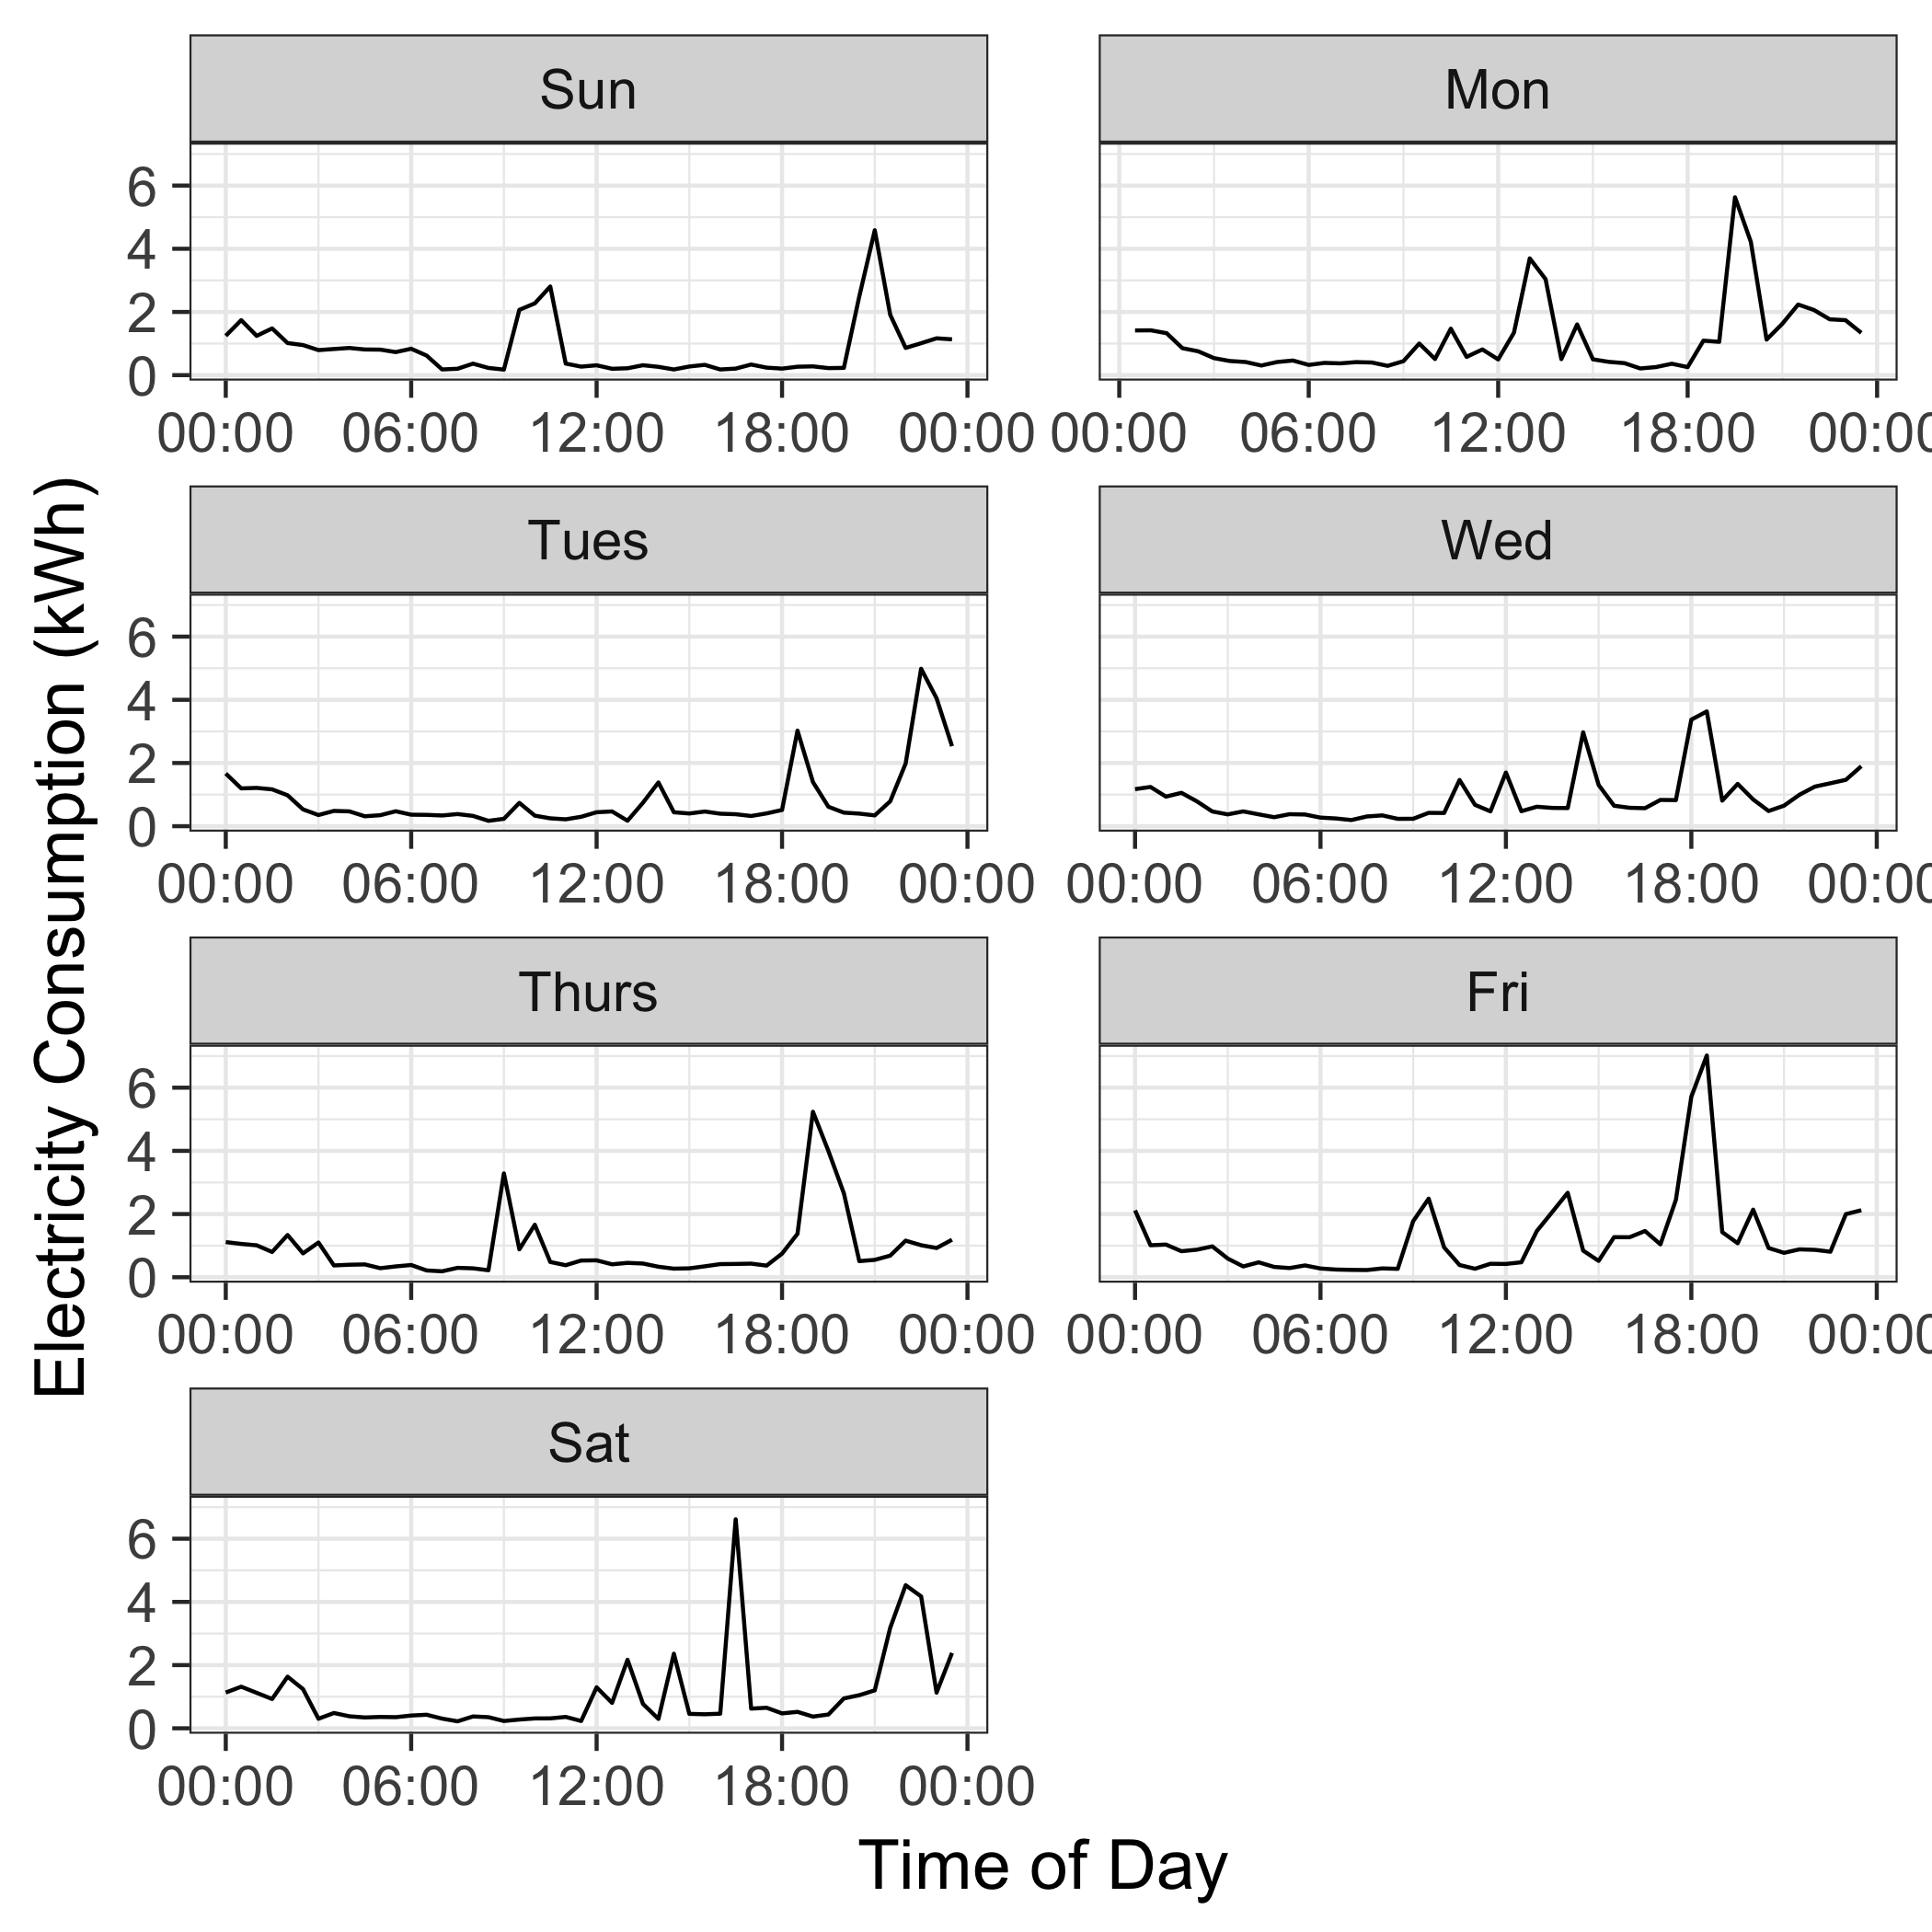
\includegraphics[width=0.6\textwidth]{Chapter5/figures/short-term-forecasting/Rplot01.png}
	\caption{Daily load profiles of a single customer over a week between 20th July 2009 and 27th July 2009. }
	\label{fig:single_user}
\end{figure}

Figure \ref{fig:single_user} demonstrates the electricity consumption profile of a single week for a single user. Whilst it can be seen that electricity usage changes significantly between days, a pattern of behaviour is exhibited. There is a large peak displayed each day in the evening, as well as a peak earlier during the day. It can, therefore, be assumed that this customer has some form of habitual behavioural pattern. 

Figure \ref{fig:multiple_users} shows eight different residential customer load profiles on the 22nd June 2009. It can be seen that the daily load profile changes between each customer. The consumers use varying quantities of electricity and at different times. 




\begin{figure}
		\centering
	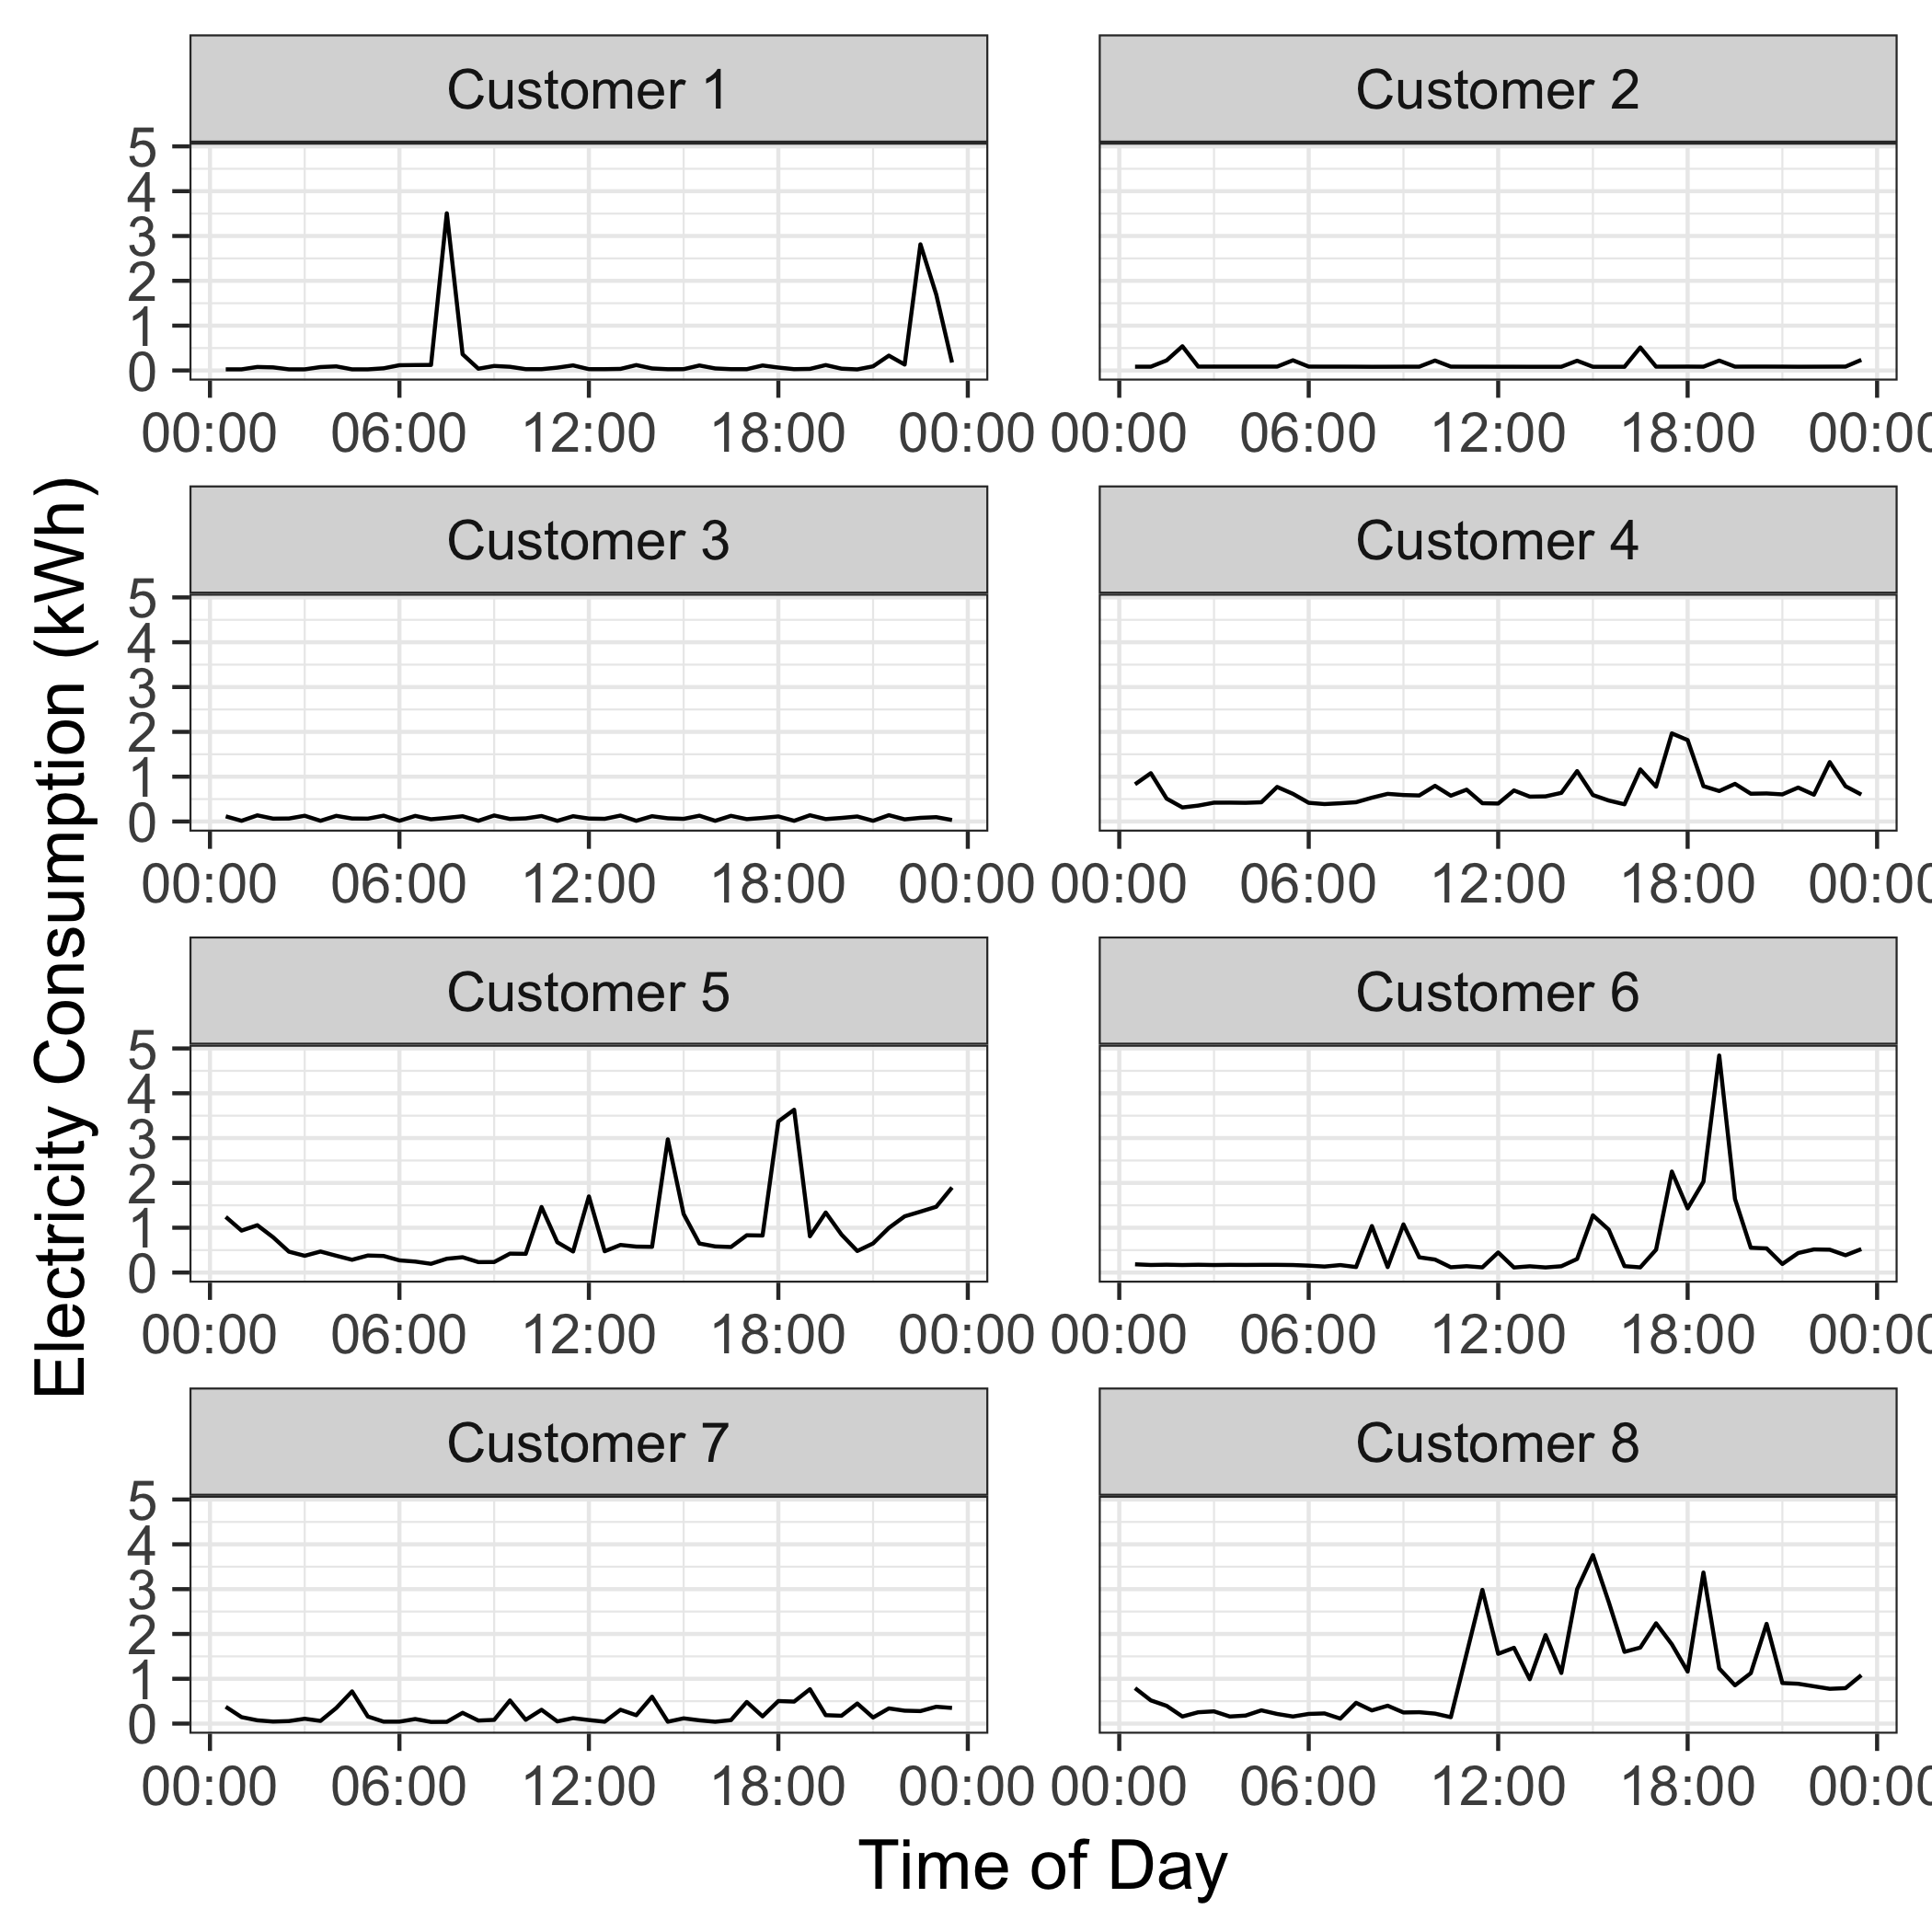
\includegraphics[width=0.6\textwidth]{Chapter5/figures/short-term-forecasting/Rplot02.png}
	\caption{Daily load profiles of different customers over a single day on the 22nd June 2009.}
	\label{fig:multiple_users}
\end{figure}

These figures display that electricity consumption changes per person, per day. To capture this variability between customer types these customers are clustered and then aggregated. Each of the different aggregated electricity consumptions should provide a less stochastic load profile, and therefore increase the accuracy of the models.

\subsubsection{Clustering}

We propose that clustering similar customer load profiles and aggregating each cluster's electricity consumption improves the accuracy of the models. 

Figure \ref{fig:similar_customers} displays four different customers with similar load profiles. Each of the users display a strong peak in electricity consumption during the evening and less consumption during the day. These customers may potentially be clustered together by the \textit{k}-means clustering algorithm.

\begin{figure}
	\centering
	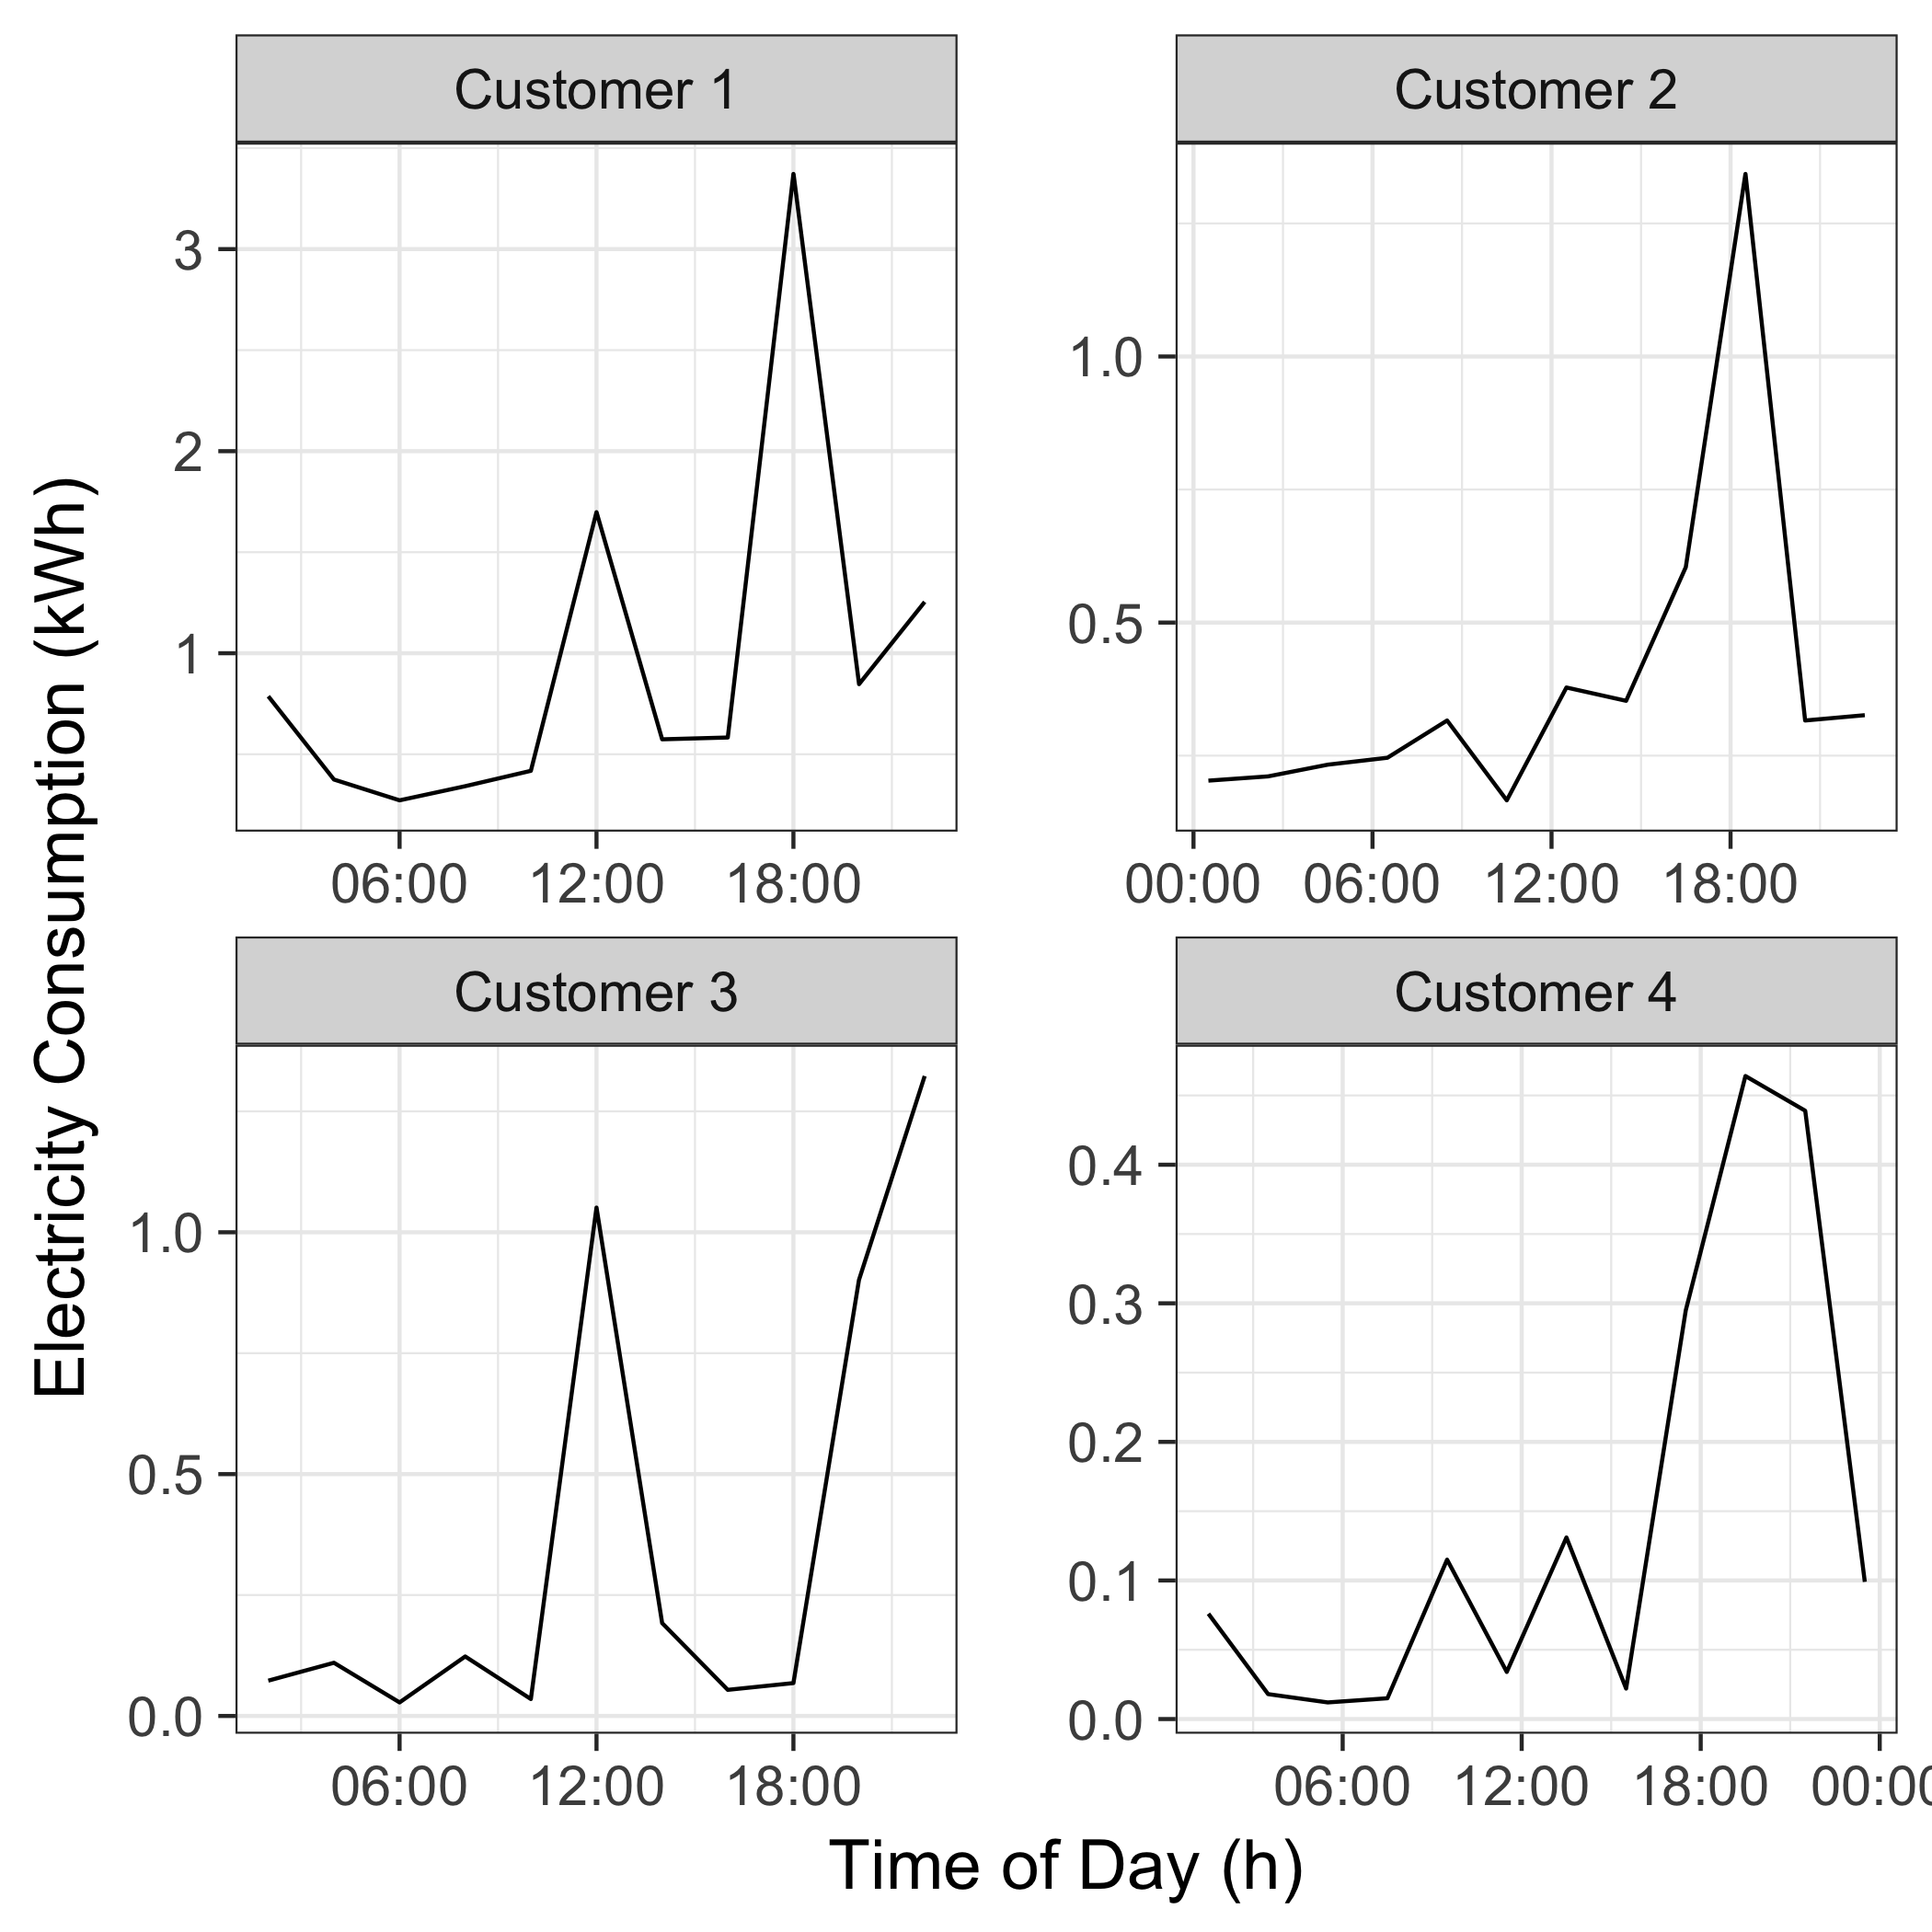
\includegraphics[width=0.6\textwidth]{Chapter5/figures/short-term-forecasting/similar_cust.png}
	\caption{Figure showing similar load profiles for four different customers on the 22nd July 2009.}
	\label{fig:similar_customers}
\end{figure}

To cluster the load profiles different options were considered. Hierarchical clustering using metrics such as Euclidean and wavelet distance metrics were evaluated \cite{BIMJ:BIMJ4710240520}, as was \textit{k}-means \cite{Forgy65}.\textit{ K}-means demonstrated to be the most robust and best-performing clustering algorithm, and thus was chosen for use in this work.

To select the optimum number of clusters (\textit{k}) cross-validation was explored. This allowed us to compare the results of each of the models and select \textit{k} with the highest MAPE accuracy.

The cross-validation method proposed, worked by trying a different number of clusters per model, and testing for the resulting MAPE. The optimum number of clusters with a low MAPE is then chosen. In this work we varied \textit{k} between 1 and 7, this range was chosen due to the fact that the error did not vary greatly past seven clusters. We fit multiple models per cluster and predicted 6 months of electricity consumption.

With \textit{k}-means clustering, it is possible that with the same initialization number of clusters, different clusters are formed. This is due to the algorithm converging at a local minima. To overcome local minima the \textit{k}-means algorithm is run multiple times and the partition with the smallest squared error is chosen \cite{Jain2010}. In our case, the \textit{k}-means clustering algorithm is run 1000 times to reduce the chance of finding a local minima. 

The clustering technique utilised in our work was a scaled input approach. The daily load profile was averaged for each customer based on each day of the training data. The data was then scaled so that households of different sizes, but with similar usage profiles were clustered together. This data, which is made up of a \textit{m-by-n} matrix, where \textit{m} is equal to the total number of meters and \textit{n} is equal to 48 (two readings for each hour in the day).

To find the optimum number of clusters it is recommended that the user selects a value of $k$ that is high enough that distinct average load profiles are displayed, however, not so high that well-clustered customers are split. By doing this, the stochasticity of the load profiles in each of the clusters will be reduced, and thus lead to the best results.


\subsubsection{Aggregating Demand}

Once each customer is assigned to their respective cluster, the total electricity consumed per cluster is aggregated. This is achieved by summing the electricity consumed at each time interval per cluster. This creates a partial system load. A different model is trained on each of the different partial system loads, and the resultant forecasts are aggregated to generate the total system load forecast. The total system load forecast is then used to evaluate the accuracy of each of the different models using MAPE. 

Random Forests, Support Vector Regression, Multilayer Perceptron neural networks and Long-Short Term Memory neural networks were evaluated, and a comparison between the different models were made. 

These models were chosen due to their ability to model multivariate non-linear relationships. They are data-driven methods and therefore suited to this type of problem.

\subsubsection{Feature Selection}

Each component of the training data is known as a feature. Features encode information from the data that may be useful in predicting electricity consumption. 

\subsubsection{Calendar Attributes}

Due to the daily, weekly and annual periodicity of the electricity consumption daily calendar attributes may be useful to model the problem. The calendar attributes included are as follows:

\begin{itemize}
	\item Hour of day
	\item Day of the month
	\item Day of the week
	\item Month
	\item Public holidays
\end{itemize}

These attributes enable the daily, weekly and annual periodicity to be taken into account by the model.

It is noted that electricity consumption changes on a public holiday such as Christmas or New Year's Eve. It is therefore proposed that public holidays in Ireland are input into the model as features. 

For testing purposes, two sets of models for Random Forests, Multilayer Perceptrons and Support Vector Regression were fit. One set omitted these calendar attributes whilst the other didn't. This is done to evaluate the importance of periodicity in electricity consumption prediction.

\subsubsection{Time Series Data}

As well as the calendar attributes it is important to consider the historical load demand. This allows the time-series element to be modelled.  

To do this, a lagged input of the previous 3 hours, the equivalent three hours from the previous day, and the equivalent 3 hours from the previous week were used. For example, to predict the electricity consumed on the 21st December 2010 at 12:00 pm the electricity between 9:00 pm and 11:30 pm on the 21st of December are used as inputs, as are the times between 9:00 pm and 12:00 pm on the 20th and 14th of December.

Long-Short Term Memory neural networks remember values over arbitrary time intervals. They can remember short-term memory over a long period of time, for this reason, 5 lagged inputs of the previous two and a half hours were used as features to the Long-Short Term Memory network.

\subsubsection{Data Representation}

Once useful information is selected we must encode the data for input into the models. To encode the day of the week seven binaries are utilised. Six of the binaries are for Monday through to Saturday. When all six binaries are equal to zero Sunday is encoded. A single binary for public holidays is included. Eleven binaries are used for month of the year, with the first eleven representing January to November, with December represented by all zeros in the calendar binaries. The current hour and date are input using a numerical attribute. The lagged data inputs, such as previous hour's electricity usage are also input using a numerical attribute for each entry, totaling 20 attributes (six half hourly entries for each 3 hour period multiplied by three days plus 2 entries for the time to be predicted on the previous day and week). Table \ref{tab:feature} displays these features.


\begin{table}
	\caption{List of Input Data for Models}
	\label{tab:feature}
	\begin{tabular}{p{3cm}p{3cm}p{8cm}}
		\toprule
		Input & Variable      & Detail description \\
		\midrule
		1     & Hour          & Single numeric input representing hour of the day                                                                                              \\
		2     & Day of month  & Single numeric input representing day of the month                                                                                             \\
		3-9   & Day of week   & Six binary digits representing calendar information regarding day of the week                                                                                            \\
		10-21 & Month         & Eleven binary digits representing calendar information regarding month                                                                                         \\
		22-42 & Lagged inputs & Twenty numeric inputs representing lagged inputs of previous 3 hours, previous 3 hours of previous day including hour to be predicted, and previous 3 hours of previous week including hour to be predicted \\
		43    & Holiday       & One binary digit representing whether the day was a public holiday  \\     \bottomrule                                                           
	\end{tabular}
\end{table}


\subsection{Experiments}

This section explores the different methods used to select the model parameters, and the tests to evaluate our models. Once the parameters were chosen the models were trained on the different clusters of residential customers. Each model was run five times to explore the variance of the results.  

\subsubsection{Support Vector Regression}

To implement a Support Vector Regression model a variety of parameters must be chosen. These parameters influence the performance of the model. The parameters were evaluated using cross-validation. To do this, the data was split 75\% into training data, and the remaining 25\% into test data. This split was chosen to balance the trade-off between having enough training data so that the model can accurately learn the underlying form of the data, but also to have enough data to test each model.

To choose the optimum support vector machine kernel cross-validation was also used. Again, with 75\% acting as the training data and 25\% as the test. The kernels compared were polynomial, radial basis function (RBF) and the linear kernel \cite{Chang2010, theodoridis2009pattern}. These were chosen due to their popularity, support and relative speed of computation.

The parameter values selected are shown in Table \ref{tab:kernel}. These parameter values were chosen from the results of cross-validation for each of the different kernels.  From the cross-validation, the linear kernel was found to be the best performing. For this reason, the linear kernel was utilised for prediction of electricity consumption in this work.

\begin{table}
	\centering
	\label{tab:kernel}
	\begin{tabular}{ccl}
		\toprule
		Kernel Type& Kernel Parameters & RMSE\\
		\midrule
		Linear & No values & 0.02103\\
		RBF & C=2, $\gamma=0.016$ & 0.0245\\
		Polynomial & C=2, $d=2, r=2$ & 0.0315 \\
		\bottomrule
	\end{tabular}
	\caption{Prediction Accuracy Based on Type of Kernel}
\end{table}


\subsubsection{Random Forest}

\begin{figure}
	\centering
	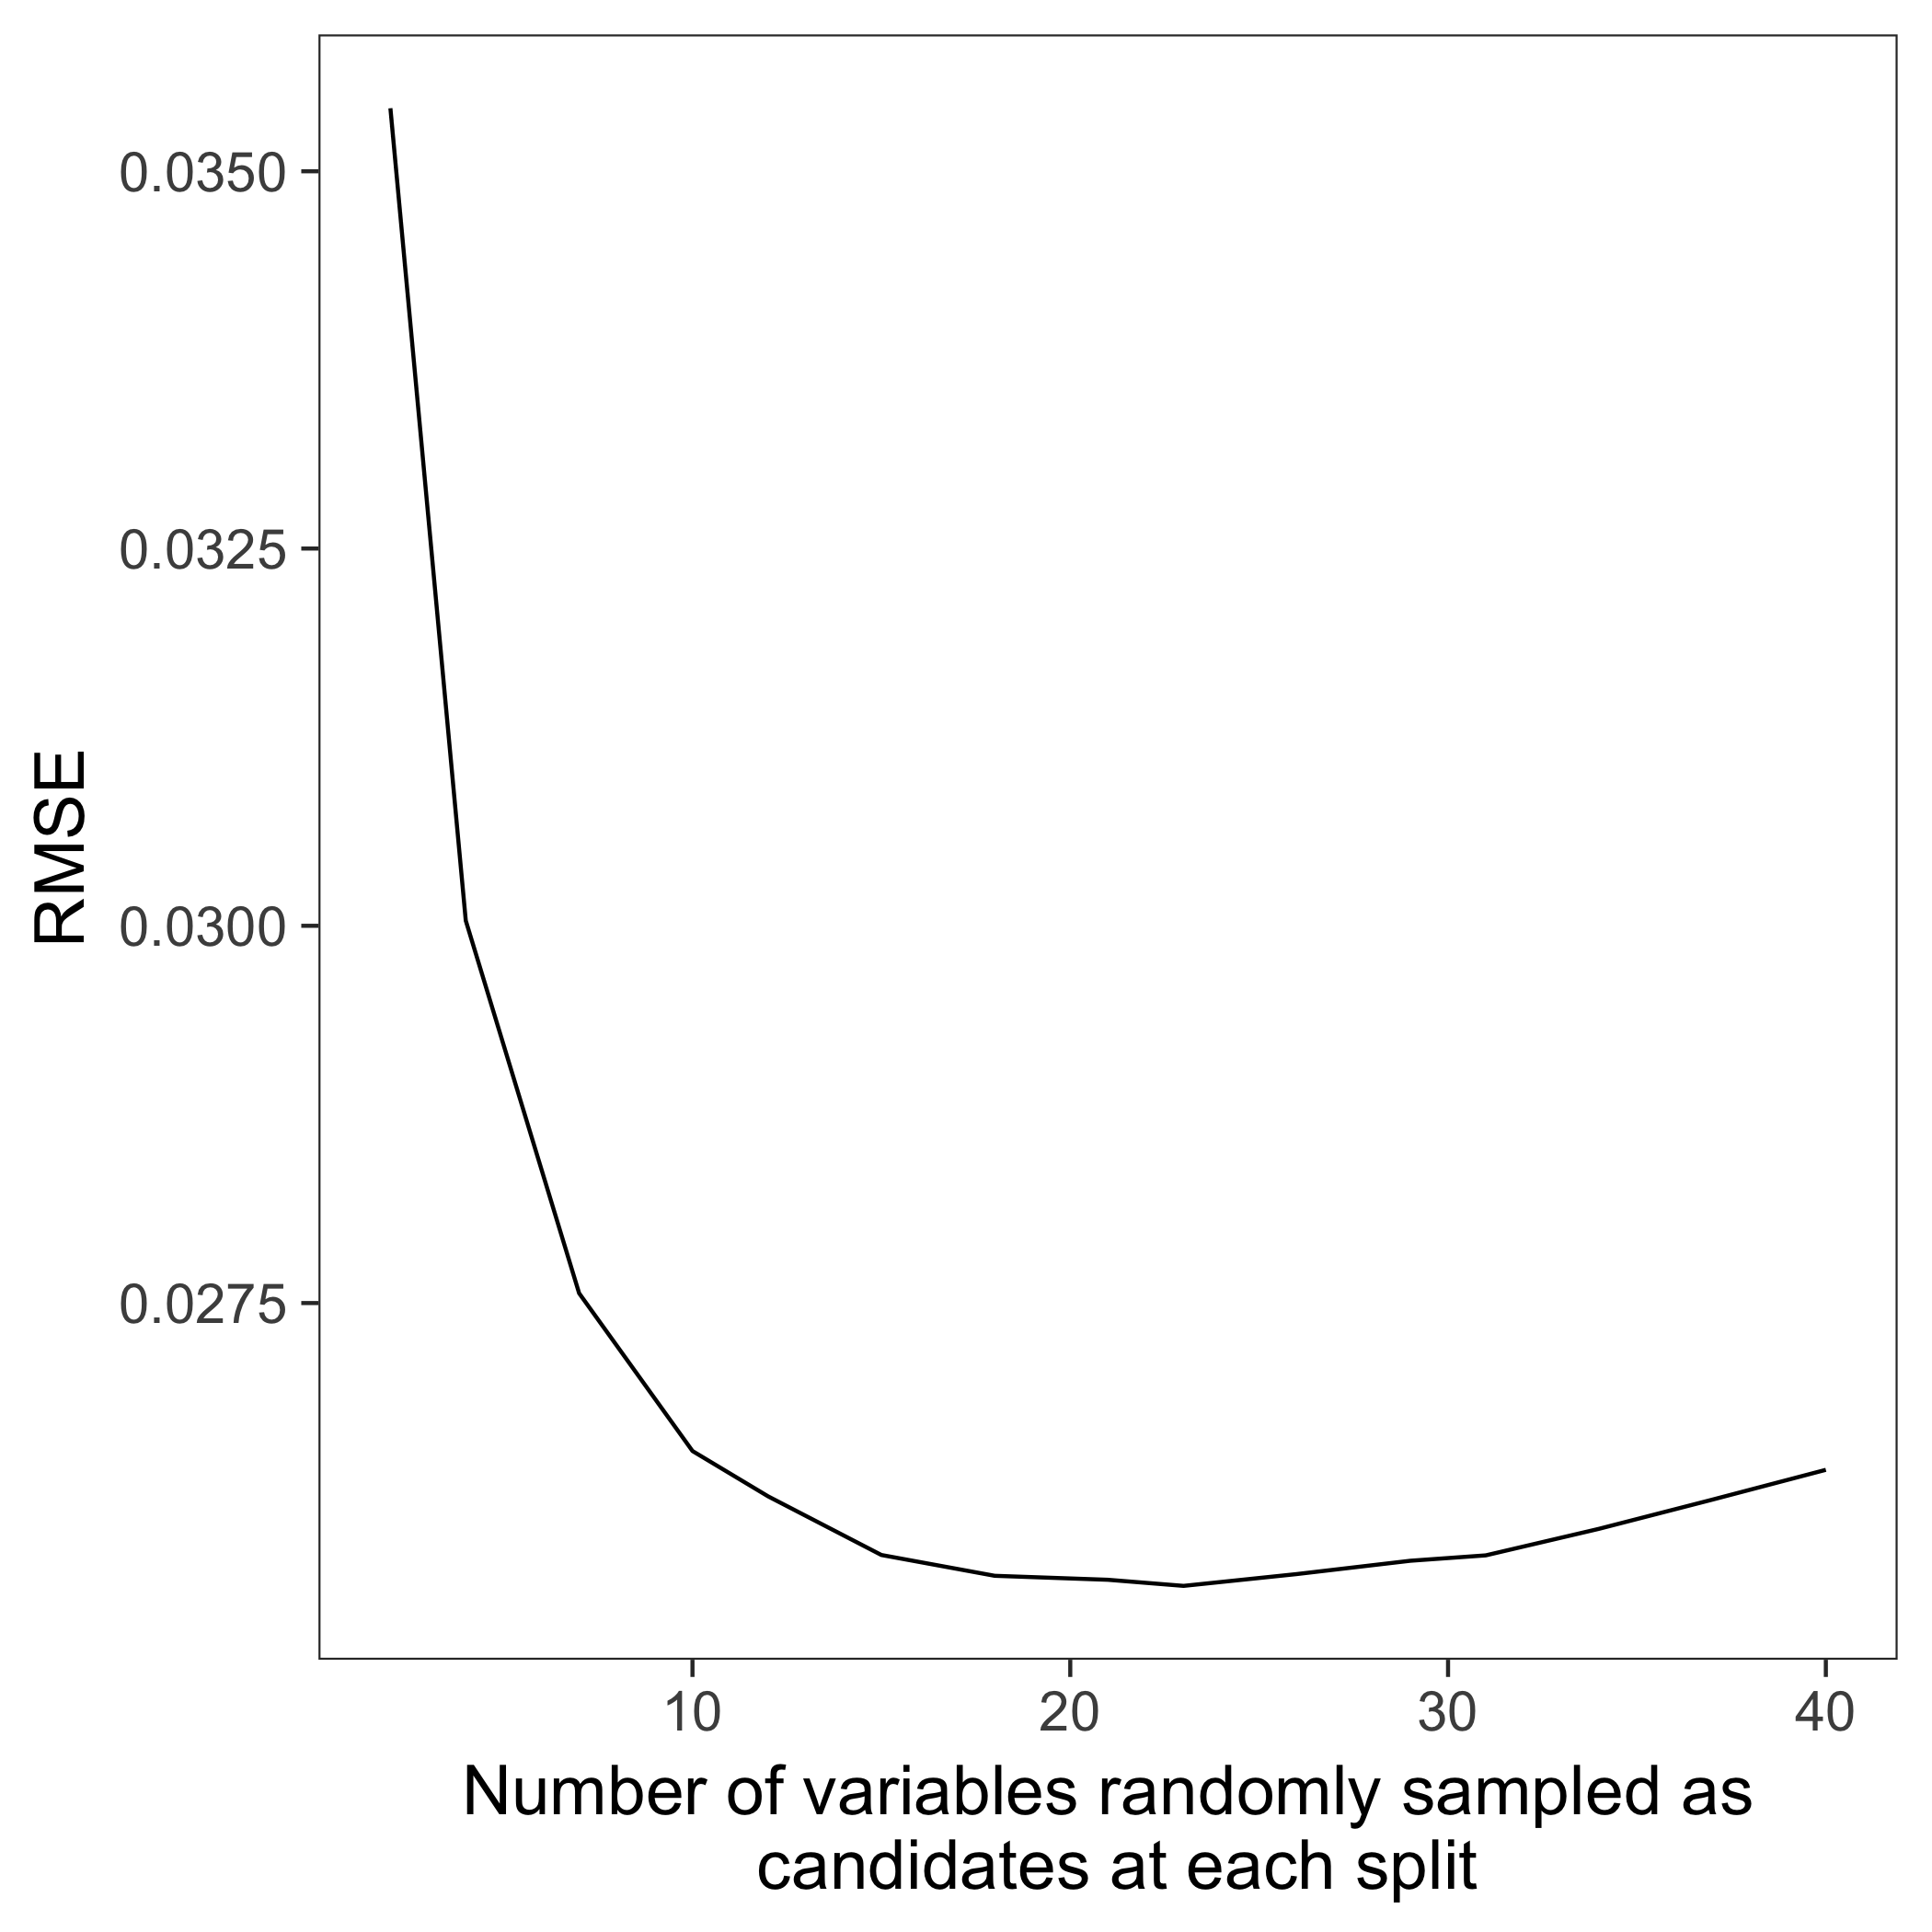
\includegraphics[width=0.6\textwidth]{Chapter5/figures/short-term-forecasting/rforest_parameter_tuning}
	\caption{RMSE vs Number of variables randomly sampled as candidates at each split in the Random Forest model.}
	\label{fig:rf_param_tune}
\end{figure}

To initialize the Random Forest algorithm with the number of variables randomly sampled as candidates at each split, cross-validation was used. Once again, 75\% of the data was used for training and the remaining 25\% for testing due to the trade-off between training and testing.

Figure \ref{fig:rf_param_tune} shows the results of tuning the parameter of the number of variables randomly sampled as candidates at each split. The optimum number was found to be 23. Either side of this value the RMSE increases. Therefore the value 23 was selected to be the number of variables randomly sampled as candidates at each split in the Random Forest model. It is proposed that the value 23 was found to be optimum due to the 20 lagged inputs, as this data is crucial for the Random Forest to learn the underlying nature of electricity load.


\subsubsection{Multilayer Perceptron}

A feed-forward Multilayer Perceptron is a common neural network architecture used for the prediction of time series data, which has comparable, and occasionally better results than statistical models \cite{Hill1994}. 

The first step when designing a Multilayer Perceptron neural network is to design the architecture. For this case, the number of input neurons is set to 41 (see Table \ref{tab:feature}). Once an input for each neuron is entered, the output layer must be designed. Due to the fact that we are forecasting only one time step ahead (30 minutes ahead) one output neuron is required.

The next step is to design the architecture of the hidden layers. To accomplish this, cross-validation is utilised as per the previous models. A maximum of 3 hidden layers were tested and the results analysed. A similar method to Fan \textit{et al.} was evaluated to choose the number of neurons and hidden layers, a technique known as the Levenberg-Marquardt technique \cite{Fan2009}. The Levenberg-Marquardt is a technique suitable for training medium-sized Artificial Neural Networks with a low mean-squared error. 

The fundamental rule is to select the minimum number of neurons in the hidden layer so as to capture the complexity of the model, but not too many as to introduce over-fitting, which results in a loss in generalization of the algorithm.

The method begins by choosing a small number of neurons and gradually increasing the number each time the model is trained and the forecast error obtained. The forecast error is monitored until an optimum value is found, to which no further improvement is noted. Once the optimum number of neurons in the layer is obtained an additional layer is added, and the same technique is used.

Using this technique an optimal architecture with three layers is obtained. The first layer contained two neurons, the second contained five, and the third contained four.



\subsubsection{LSTM}

To initialize the LSTM, cross-validation was used to select the number of stacked layers and memory units. Similarly to the technique used for the Multilayer Perceptron, the Levenberg-Marquardt was used. The optimum number of layers was found to be 2, with a total of 50 memory units. Different combinations of layers and memory units displayed worse results.



\subsection{Results}


\begin{figure}
	\centering
	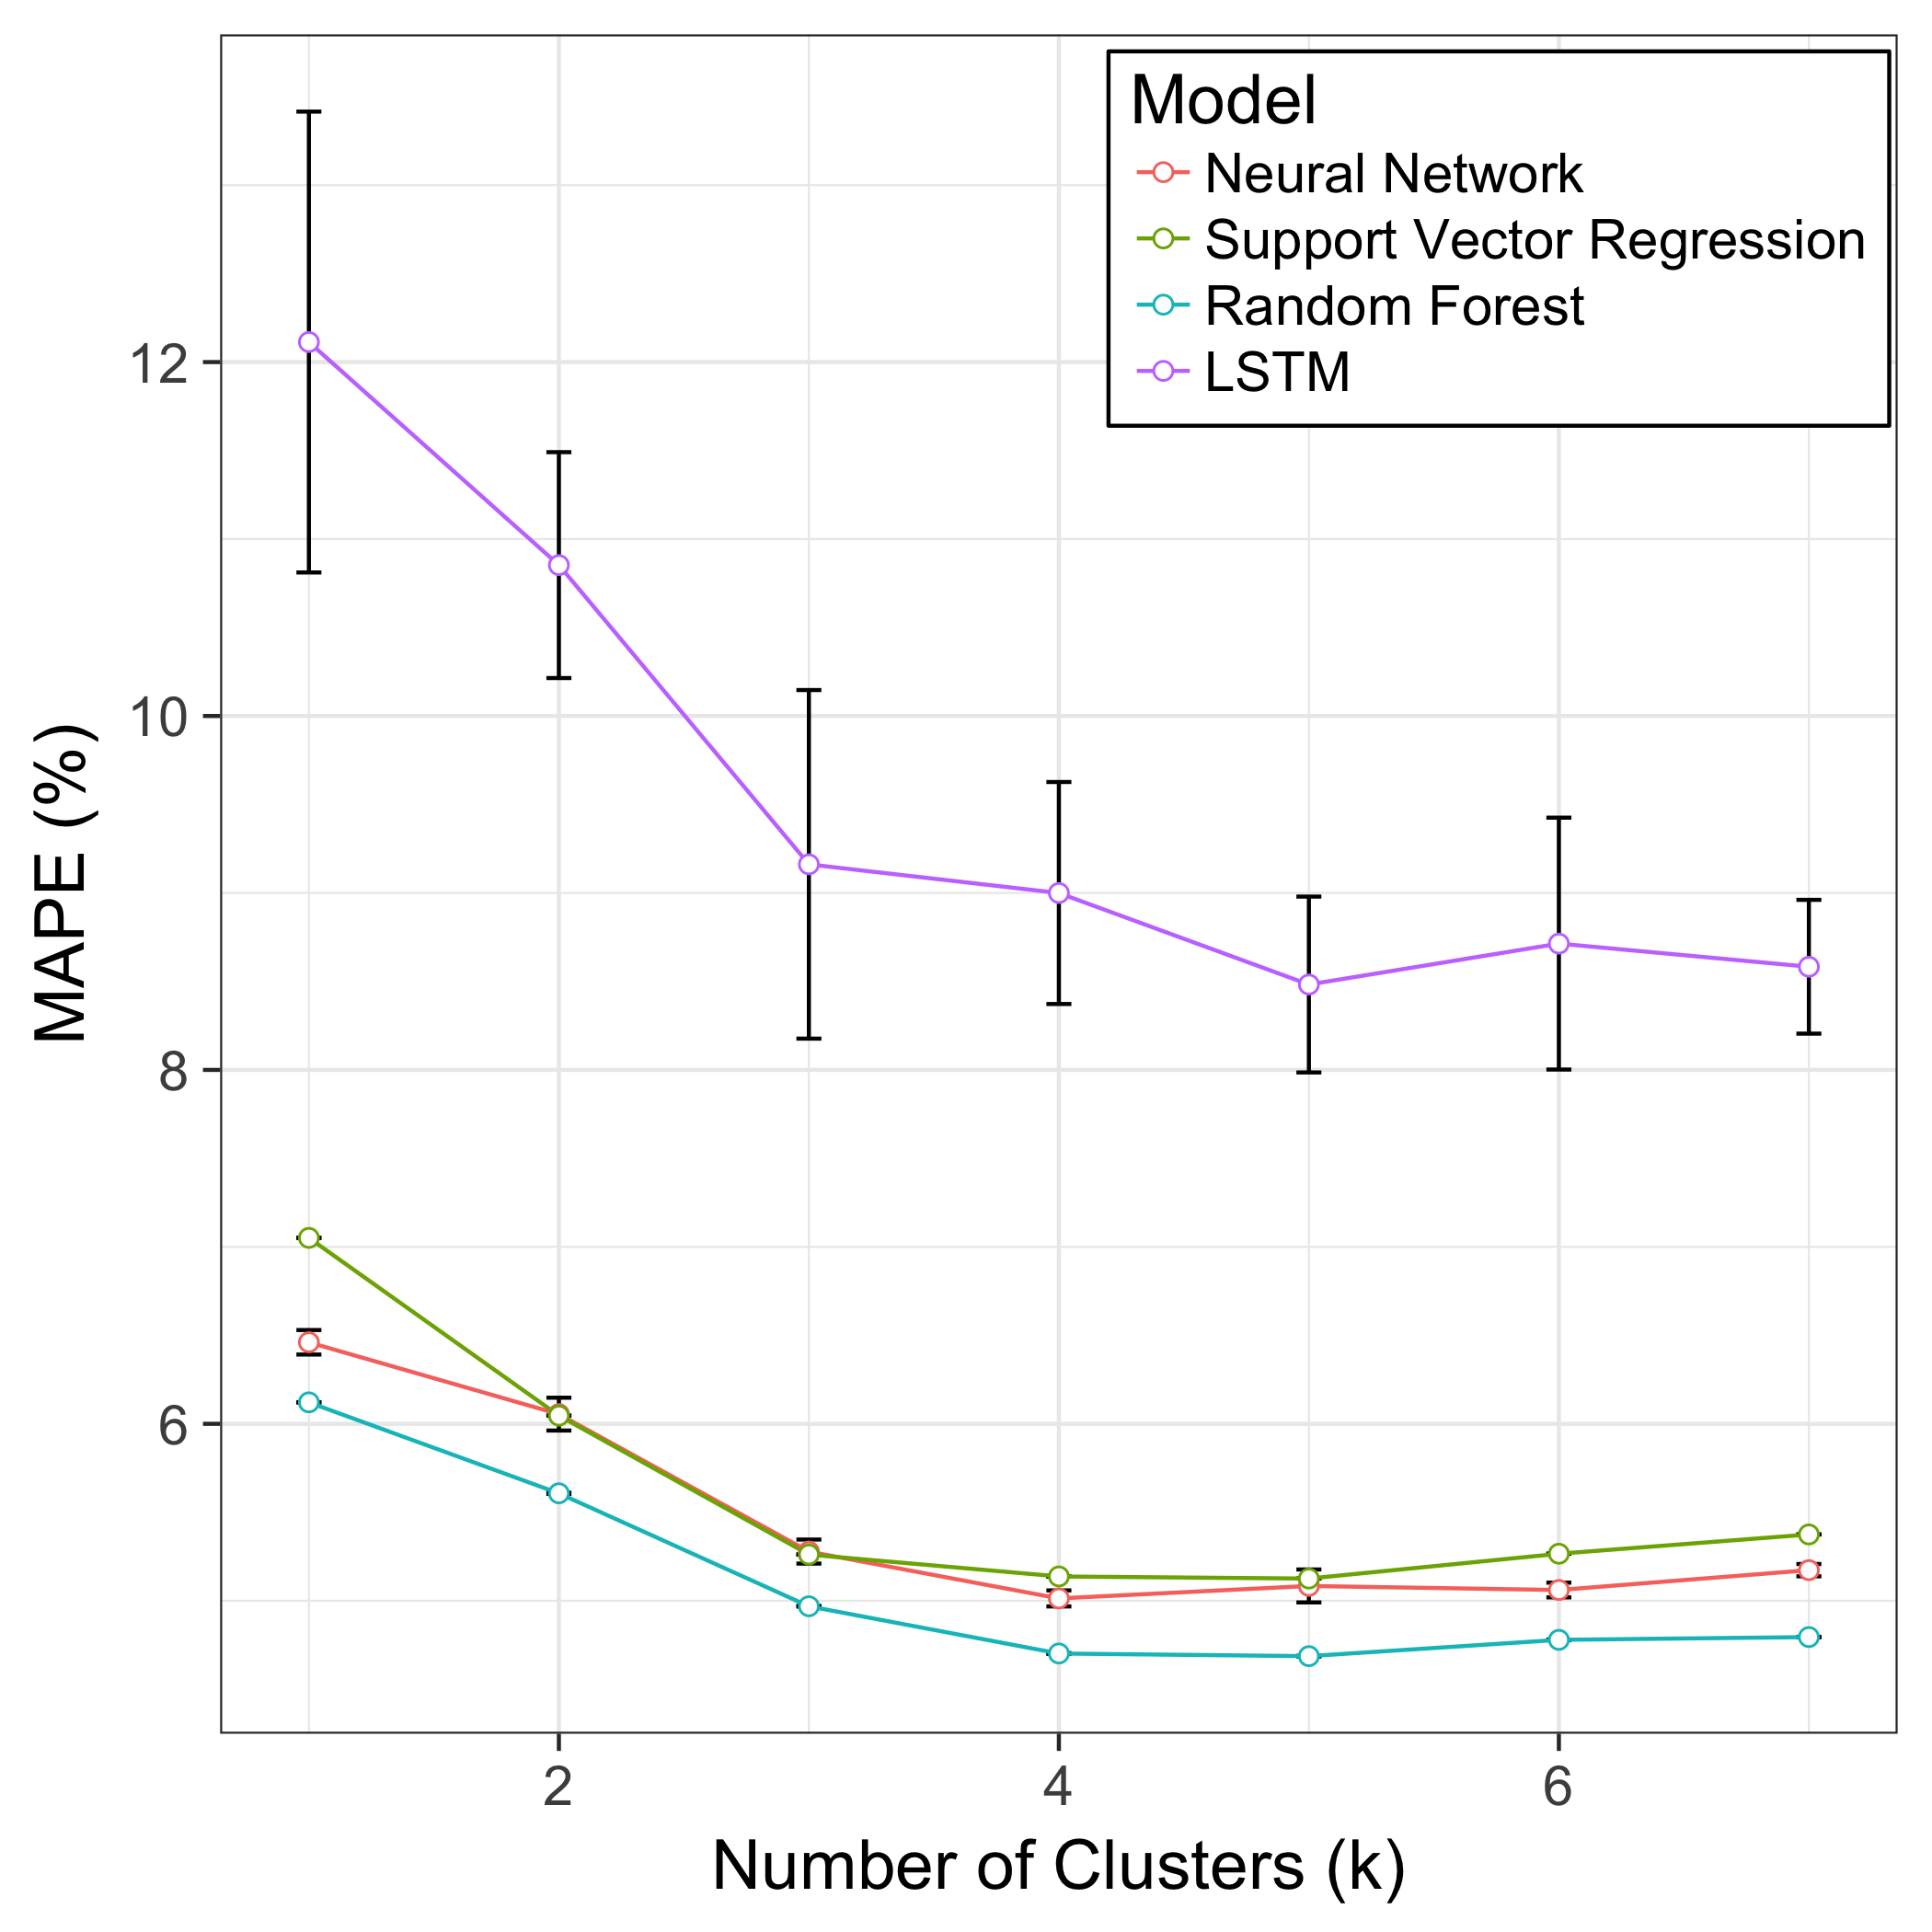
\includegraphics[width=0.6\textwidth]{Chapter5/figures/short-term-forecasting/results.png}
	\caption{Comparison of accuracy of models forecasting electricity with varying number of clusters.}
	\label{fig:results}
\end{figure}

\begin{figure}
	\centering
	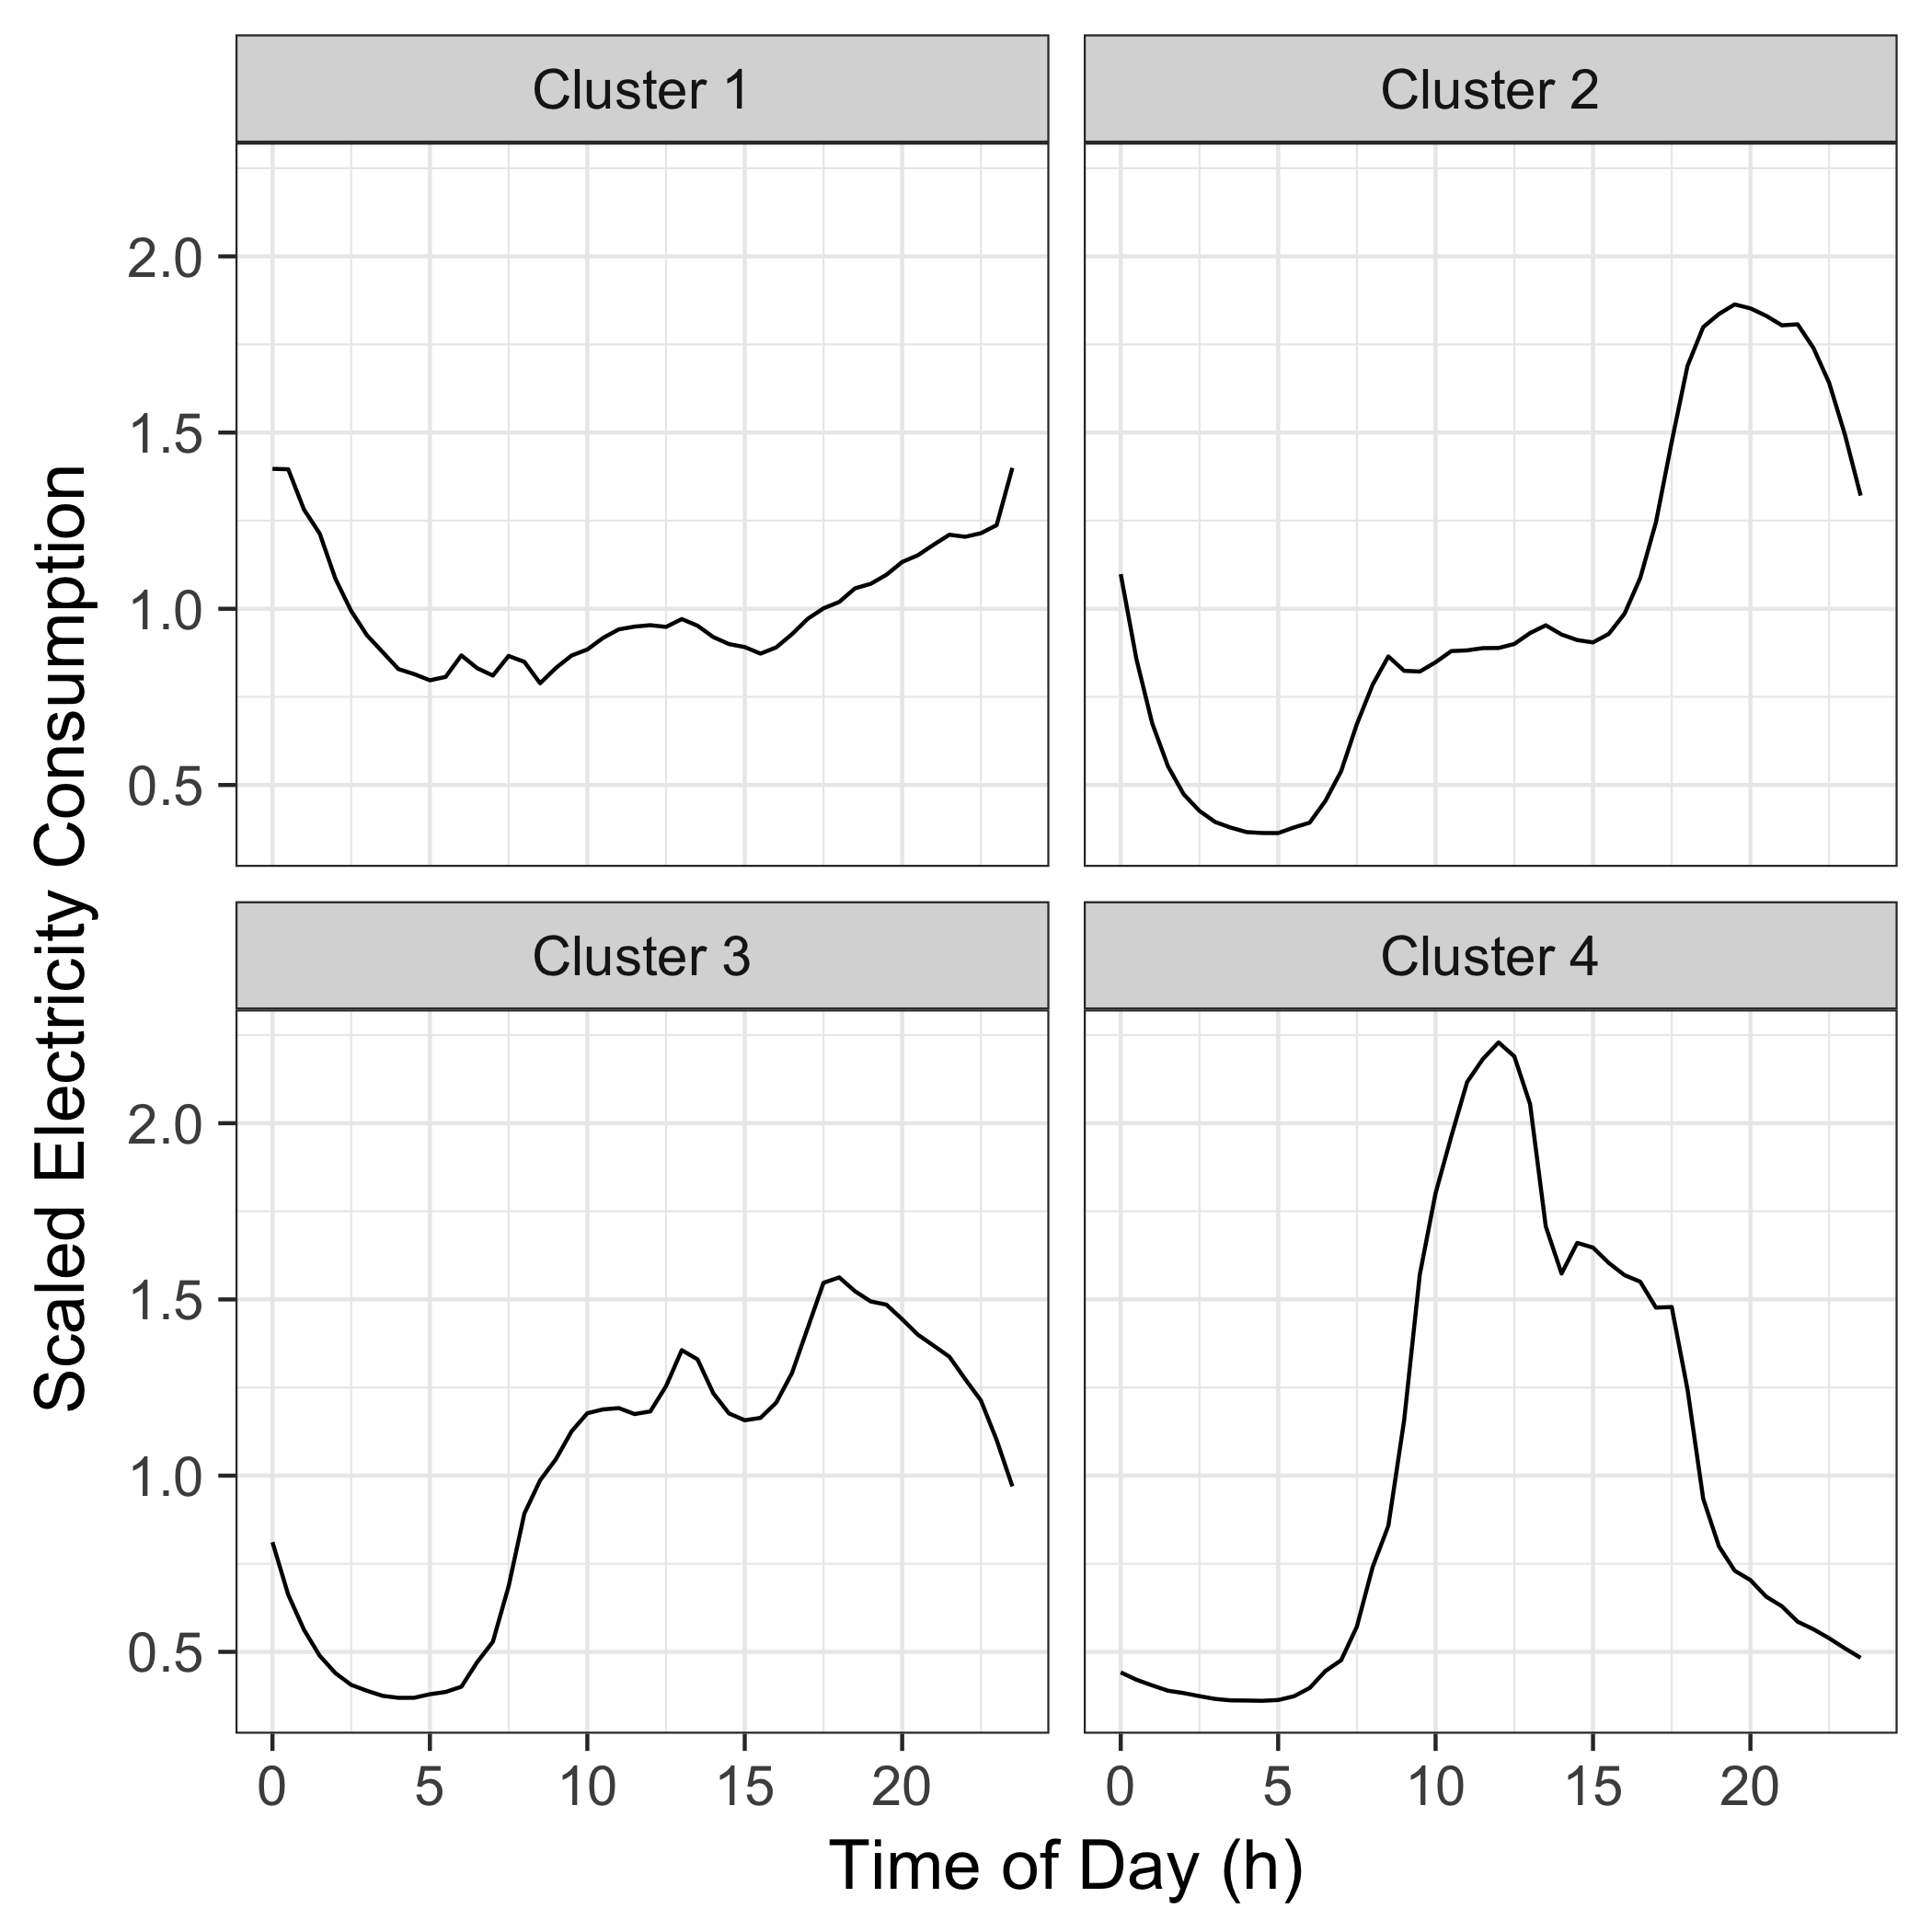
\includegraphics[width=0.6\textwidth]{Chapter5/figures/short-term-forecasting/Cluster_Centres.png}
	\caption{Average load profile for each cluster.}
	\label{fig:clustercentre}
\end{figure}

To test the accuracy of the trained model the data was split into a training and test set. The data between the 14th of July 2009 and the 15th of June 2010 was used as the training data, whilst the data between the 15th of June 2010 and 31st of December 2010 was used for testing purposes. The test set is separate from the training set and not used during training. 

28 independent forecasting models are constructed for each of the Random Forests, Support Vector Regression, LSTMs and Multilayer Perceptron neural networks for each of the groups with \textit{k} varying from 1 to 7. This was done to determine the optimal number of clusters.  Each of the 28 models are trained independently, five times each so that the standard deviation results of MAPE for each cluster could be displayed. We evaluated the MAPE of the overall prediction. 

Figure \ref{fig:results} displays the accuracy of the models trained at different numbers of clusters (\textit{k}). The results demonstrate that introducing clusters to group similar customers improve results in all cases. The optimum value for \textit{k} for Random Forests, Support Vector Regression and neural networks was shown to be four for our dataset. After this, the accuracy diminishes slightly. The error bars shown in Figure \ref{fig:results} show a small variance in MAPE in \acrshort{svr}s, ANNs and Random Forests. However, the MAPE of the LSTMs seem to vary by up to 11\% in the five models run. 

Figure \ref{fig:calendar_attr} demonstrates the impact of using calendar attributes such as month, day of the month, and day of the week on prediction accuracy. The results show an increase in prediction accuracy of 6\% for neural networks, 4\% for Random Forests and 1\% for support vector regression when taking into account these variables. It is proposed that the ability for the models to take into account the cyclic yearly, monthly and weekly behaviour improves the results.

\begin{figure}
	\centering
	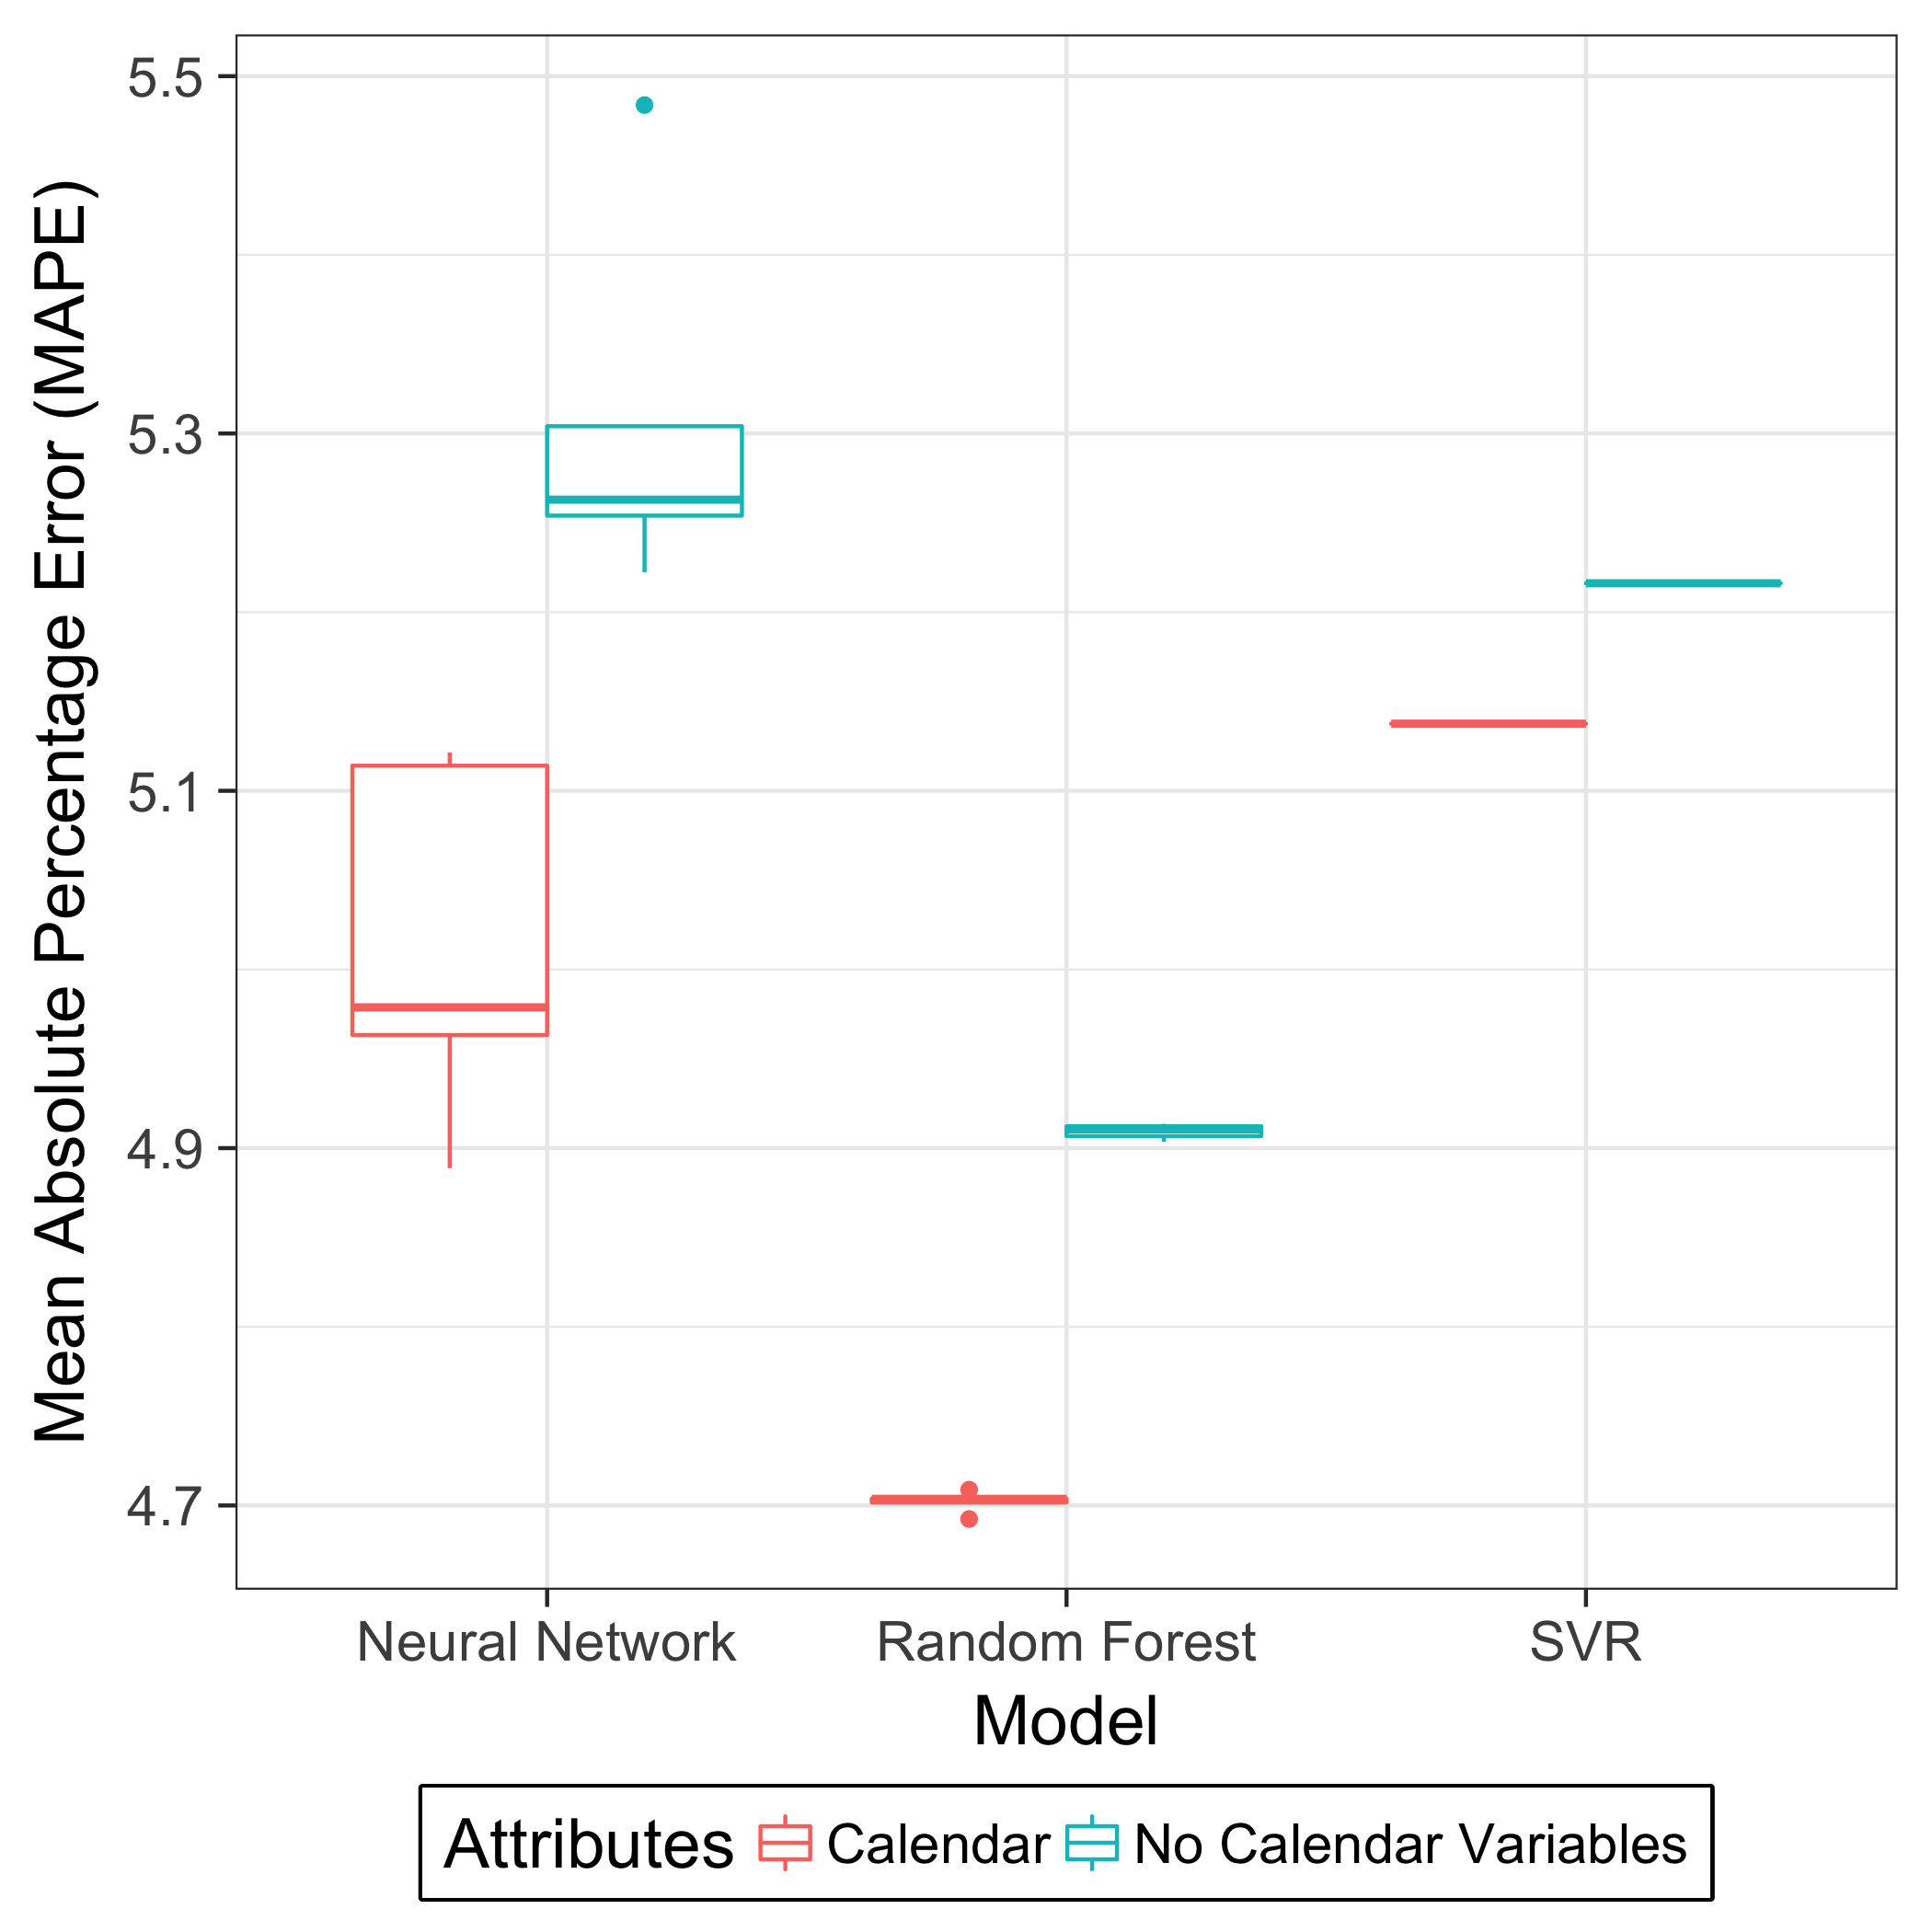
\includegraphics[width=0.6\textwidth]{Chapter5/figures/short-term-forecasting/calendar_attr.png}
	\caption{Comparison of accuracy of models with or without calendar attributes.}
	\label{fig:calendar_attr}
\end{figure}



Figure \ref{fig:clustercentre} shows the average load profiles of different clusters when $k=4$. It is proposed that the optimum number of clusters is four due to the distinct load profiles that can be seen in Figure \ref{fig:clustercentre}. The four different distinct patterns seen are high night time use in cluster 1, a typical residential load profile is shown in cluster 2, a spread of usage in cluster 3, and high daytime usage in cluster 4. At $k=3$ these distinct patterns are not adequately clustered, and at $k=5$ one of the distinct clusters are split, leading to an increase in stochasticity.

It is true that the optimum number of clusters will vary for different datasets. Whilst residential smart meter datasets may be similar, it is entirely possible that different geographies display different usage characteristics based on factors such as culture, temperature and economical reasons. It is therefore important to choose an optimal number of clusters for each dataset.

The results demonstrate that SVR, Random Forests and the Multilayer Perceptrons have a similar overall accuracy. The LSTM shows a similar pattern in increasing accuracy with number of clusters. However, the Random Forest seems to outperform each of the models at every point. This may be due, in part, to the internal operation of the Random Forest which undertakes its own cross-validation using out-of-bag samples and only having a few tuning parameters. 

It has been shown that neural networks, SVR and Random Forests all perform within an adequate range of predicting electricity consumption. Whilst LSTMs perform poorly. This may be due to the features given to the LSTM which only had previous two and a half hours of data as input. 

However, it is well known that the best machine learning technique for predicting energy consumption cannot be chosen \textit{a priori}. Therefore it is necessary to compare different techniques to find the best solution to a particular regression problem \cite{Ahmad2017}.

For this work, the training time was tested by timing how long the models would be fit to create one cluster (single model trained on the training set). The Support Vector Regression took much less time than all of the other methods, whereas the LSTM took the longest. The Artificial Neural Network required 9 minutes and 5 seconds to run. The Support Vector Regression model required 3 minutes and 32 seconds to run. The Random Forest, on the same data, required 9 minutes and 44 seconds to run, whilst the LSTM took 12 minutes 55 seconds. 


\subsection{Conclusion}

The availability of high granularity data produced by the smart grid enables network operators to gain greater insights into their customer behaviour and electricity usage. This enables them to improve customer experience, utility operations and power management. We demonstrated that implementing the \textit{k}-means clustering algorithm to group similar customers improved the accuracy of every one of the different models tested. Distinct models were trained for each of the clusters and the individual forecasts aggregated for the total aggregated forecast. It was found that Random Forests outperformed  the other models at all levels of clustering and that the optimum number of clusters was 4. Whilst the dataset used focused on residential data it is expected that applying a similar clustering technique on commercial properties would have a similar effect.

In future work, we will look into the features that best aid in the forecasting of electricity consumption, try a wider variety of models in an ensemble manner and try different clustering techniques such as self-organizing maps (SOM) to obtain better accuracy measures. We will also compare different prediction error measures.

To utilize more of the data and increase the number of models trained these results could be run in parallel and on the cloud in future.


\section{Day-ahead forecasting}
\label{forecast:sec:longterm}

In this section we expand on the work undertaken in Section \ref{forecast:sec:shortterm} by utilising further time-series prediction algorithms, including online machine learning methods. We take the error distributions and perturb the exogenous electricity demand of ElecSim, and observe the long-term impacts of poor error forecasts on the UK electricity market. It should be noted that this could work for any decentralised electricity market. 


\subsection{Methods}
\label{sec:methods}

%In this Section, we present the methodology for the approach taken in this paper. The work here was run on a MacBook Pro with a 2.3GHz 8-Core Intel Core i9 processor, with 32GB 2667 MHz DDR4 RAM.

\subsubsection{Data preparation}

Similarly to our previous work in Chapter \ref{chapter:elecsim} \cite{Kell2018a}, we selected a number of calendar attributes and demand data from the GB National Grid Status dataset provided by the electricity market settlement company Elexon, and the University of Sheffield \cite{gbnationalgridstatus_2019}. This dataset contained data between the years 2011-2018 for the United Kingdom. The calendar attributes used as predictors to the models were hour, month, day of the week, day of the month and year. These attributes allow us to account for the periodicity of the data within each day, month and year.

It is also the case that electricity demand on a public holiday which falls on a weekday is dissimilar to load behaviours of ordinary weekdays \cite{Kim2000}. We, therefore, marked each holiday day to allow the model to account for this.

As demand data is highly correlated with historical demand, we lagged the input demand data. In this context, the lagged data is where we provide data of previous time steps at the input. For example, for predicting $t+1$, we use $n$ inputs: {$t,t-1,t-2,\ldots,t-n$}. This enabled us to take into account correlations on previous days, weeks and the previous month. Specifically, we used the previous 28 hours before the time step to be predicted for the previous 1st, 2nd, 7th and 30th day. We chose this as we believe that the previous two days were the most relevant to the day to be predicted, as well as the weekday of the previous week and the previous month. We chose the previous 28 hours to account for a full day, plus an additional 4 hours to account for the previous day's correlation with the day to be predicted. We could have increased the number of days provided to the algorithm. However, due to time and computational constraints, we used our previously described intuition for lagged data selection. The number of lagged inputs to trial increases exponentially with each additional day added, therefore making the problem intractable when also trialling such a high number of algorithms and hyperparameters. 

In addition to this, we marked each of the days with their respective seven seasons. These seasons were defined by the National Grid Short Term Operating Reserve (STOR) Market Information Report \cite{ESO2019}. These differ from the traditional four seasons by splitting autumn into two further seasons, and winter into three seasons. Finally, to predict a full 24-hours ahead, we used 24 different models, 1 for each hour of the day. 


The data is standardized and normalized using min-max scaling between -1 and 1 before training and predicting with the model. This is due to the fact that the inputs such as day of the week, hour of day are significantly smaller than that of demand. Therefore, the demand will influence the result more due to its larger value. However, this does not necessarily mean that demand has greater predictive power.

\subsubsection{Algorithm Tuning}

To find the optimum hyperparameters, cross-validation is used. As this time-series data was correlated in the time-domain, we took the first six years of data (2011-2017) for training and tested on the remaining year of data (2017-2018).

Each machine learning algorithm has a different set of parameters to tune. To tune the parameters in this work, we used a grid search method. Grid search is a brute force approach that trials each combination of parameters at our choosing; however, for our search space this was small enough to make other approaches not worth the additional effort.

Tables \ref{table:hyperparameter-tuning-offline} and \ref{table:hyperparameter-tuning-online} display each of the models and respective parameters that were used in the grid search. Table \ref{table:hyperparameter-tuning-offline} shows the offline machine learning methods, whereas Table \ref{table:hyperparameter-tuning-online} displays the online machine learning methods. Each of the parameters within the columns ``Values'' are trialled with every other parameter.

Whilst there is room to increase the total number of parameters, due to the exponential nature of grid-search, we chose a smaller subset of hyperparameters, and a larger number of regressor types. Specifically, with neural networks, there is a possibility to extend the number of layers as well as the number of neurons, to use a technique called deep learning. Deep learning is a class of neural networks that use multiple layers to extract higher levels of features from the input. For this work, however, we decided to trial a large number of different models, instead of a large number of different configurations for neural networks.



%\begin{landscape}
\begin{sidewaystable*}[p]
	\centering
	%\begin{adjustbox}{angle=90}
	\begin{tabular}{@{}lllllll@{}}
		\toprule
		\textbf{Regressor Type} & \textbf{Parameters} & \textbf{Values}   & \textbf{Parameters} & \textbf{Values} & \textbf{Parameters} & \textbf{Values}       \\ \midrule
		Linear                  & N/A                 & N/A               &                     &                 &                     &                       \\
		Lasso                   & N/A                 & N/A               &                     &                 &                     &                       \\
		Elastic Net             & N/A                 & N/A               &                     &                 &                     &                       \\
		Least-Angle             & N/A                 & N/A               &                     &                 &                     &                       \\
		Extra Trees             & \# Estimators       & {[}16, 32{]}      &                     &                 &                     &                       \\
		Random Forest           & \# Estimators       & {[}16, 32{]}      &                     &                 &                     &                       \\
		AdaBoost                & \# Estimators       & {[}16, 32{]}      &                     &                 &                     &                       \\
		Gradient Boosting       & \# Estimators       & {[}16, 32{]}      & learning rate       & {[}0.8, 1.0{]}  &                     &                       \\
		Support Vector          & Kernel              & {[}linear, rbf{]} & C                   & {[}1, 10{]}     & Gamma               & {[}0.001, 0.0001{]}   \\
		Multilayer Perceptron   & Activation function & {[}tanh, relu{]}  & hidden layer sizes  & {[}1, 50{]}     & Alpha               & {[}0.00005, 0.0005{]} \\
		K-Neighbours            & \# Neighbours       & {[}5, 20, 50{]}   &                     &                 &                     &                       \\ \bottomrule
	\end{tabular}%
	%\end{adjustbox}
	\caption{Hyperparameters for offline machine learning regression algorithms}
	\label{table:hyperparameter-tuning-offline}
	
	%\end{sidewaystable}%
	
	%\quad
	\qquad
	\qquad
	\qquad
	\qquad
	\qquad
	\qquad
	\qquad
	\qquad
	\qquad
	
	%\begin{sidewaystable}
	\centering
	%\begin{adjustbox}{angle=90}
	\begin{tabular}{@{}llp{2.5cm}lllp{1.6cm}@{}}
		\toprule
		\textbf{Regressor Type} & \textbf{Parameters} & \textbf{Values}                                  & \textbf{Parameters} & \textbf{Values}   & \textbf{Parameters} & \textbf{Values}        \\ \midrule
		Linear                  & N/A                 & N/A                                              &                     &                   &                     &                        \\
		Box-Cox                 & Power               & {[}0.1, 0.05, 0.01{]}                            &                     &                   &                     &                        \\
		Multilayer Perceptron   & Hidden layer sizes  & {[}(10, 50, 100), (10),  (20), (50), (10, 50){]} & 
		&                   &                     &                        \\ 
		Passive Aggressive      & C                   & {[}0.1, 1, 2{]}                                  & Fit intercept?      & {[}True, False{]} & Max iterations      & {[}1, 10, 100, 1000{]} \\
		\bottomrule
	\end{tabular}%
	%\end{adjustbox}
	\caption{Hyperparameters for online machine learning regression algorithms}
	\label{table:hyperparameter-tuning-online}
\end{sidewaystable*}%
%\end{landscape}


\subsubsection{Prediction Residuals in ElecSim}

Each of the previously mentioned models trialled will have a certain degree of error. Prediction residuals are the difference between the estimated and actual values. We collect the prediction residuals to form a distribution for each of the models. We then trial 80 different closed-form distributions to see which of the distributions best fits the residuals from each of the models. These 80 distributions were chosen due to their implementation in scikit-learn \cite{scikit-learn}.

Once each of the prediction residual distributions are fit with a sensible closed-form distribution, we sample from this new distribution and perturb the demand for the electricity market at each time step within ElecSim.

By perturbing the market by the residuals, we can observe what the effects are of incorrect predictions of demand in an electricity market using the long-term electricity market model, ElecSim. We are able to understand the differences that prediction residuals have on long-term investment decisions as well as generators utilized.




\subsection{Results}
\label{sec:results}

In this Section, we detail the accuracy of the algorithms and statistical models to predict 24 hours ahead for the day-ahead market. In addition to this, we display the impact of the errors on electricity generation investment and electricity mix from the years 2018 to 2035 using the agent-based model ElecSim.



\subsubsection{Offline Machine Learning}

To generate these results, we use a training set to train the data, and a test set to see how well each algorithm performs on the testing data. That is, how well the algorithm can predict data it is yet to see. In our case, the training data was from 2011 to 2017, and the testing data was from 2017 to 2018.

Figure \ref{fig:beis_elecsim_historic_comparison} displays the mean absolute error of each of the offline statistical and machine learning models on a log scale. It can be seen that the different models have varying degrees of success. The least accurate models were linear regression, the multilayer perceptron (MLP) model and the Least Angle Regression (LARS). These all have mean absolute errors over 10,000MWh. This error would be prohibitively high in practice; the max tendered national grid reserve is 6,000MWh, while the average tendered national grid reserve is 2,000MWh \cite{ESO2019}.

A number of models perform well, with a low mean absolute error. These include the Lasso, gradient Boosting Regressor and K-neighbours regressor. The best model, similar to \cite{Kell2018a}, was the decision tree-based model, Extra Trees Regressor, with a mean absolute error of $1,604$MWh. This level is well within the average national grid reserve of 2,000MWh.



\begin{figure}
	\centering
	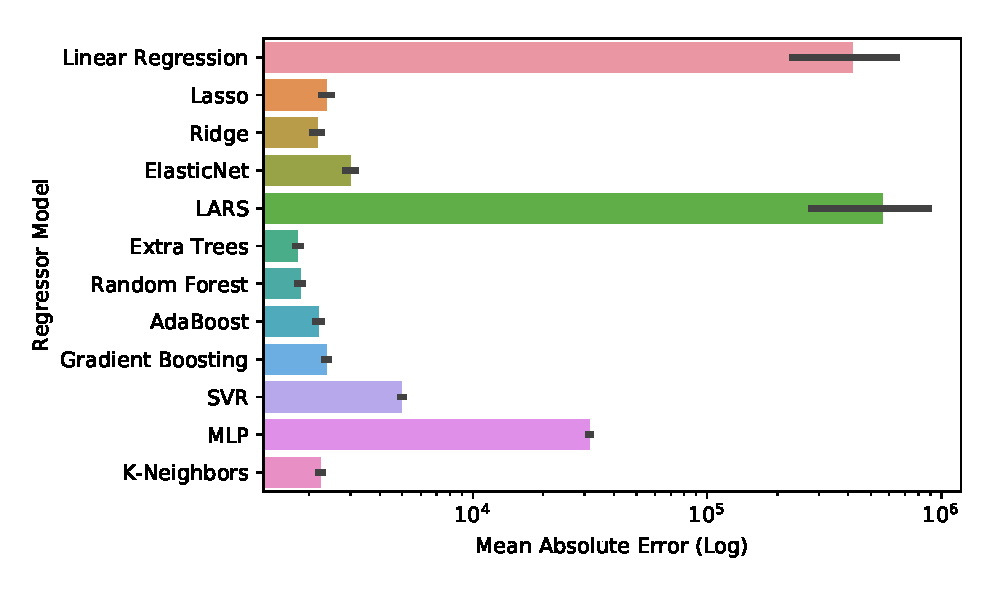
\includegraphics[width=0.65\columnwidth]{Chapter5/figures/market-forecasting/results/offline_model_mae.eps}
	\caption{Offline models mean absolute error comparison, with 95\% confidence interval for 5 runs of each model.}
	\label{fig:beis_elecsim_historic_comparison}
\end{figure}


%\begin{figure}
%\centering
%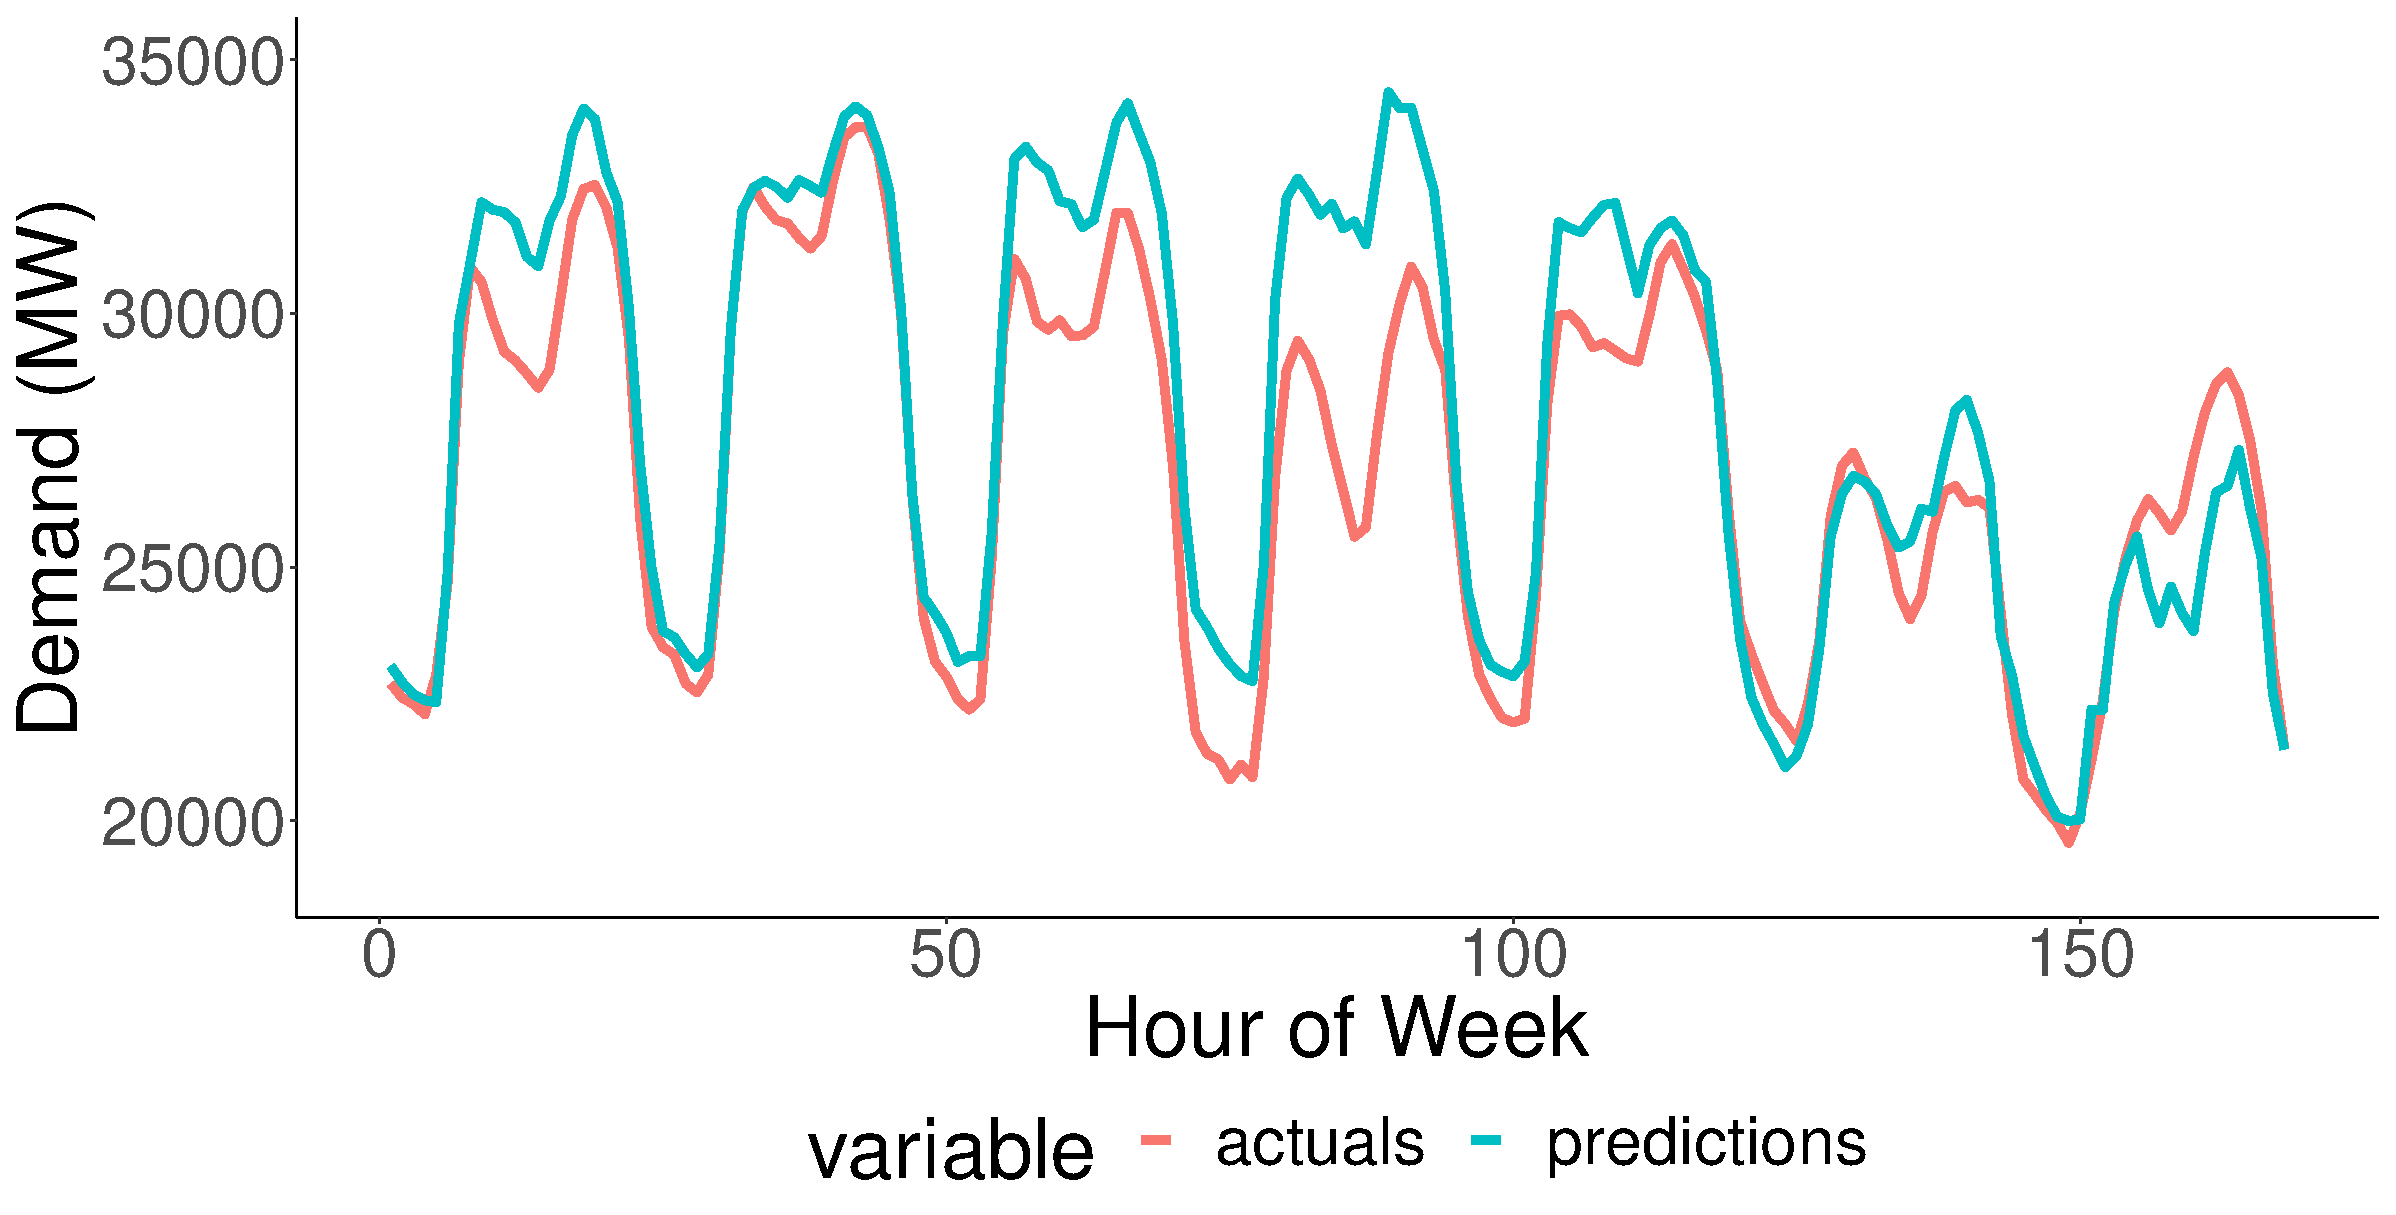
\includegraphics[width=\columnwidth]{Chapter5/figures/market-forecasting/results/offline_rf_actual_predicted.eps}
%\caption{Best offline machine learning learning algorithm (Extra Trees Regressor) predictions versus actuals for a week in June 2018.}
%\label{fig:best_offline_learning_day_simulation}
%\end{figure}

Figure \ref{fig:best_offline_learning_day_distribution} displays the distribution of the best offline machine result (Extra Trees Regressor). It can be seen that the max tendered national grid reserve falls well above the 5\% and 95\% percentiles. However, there are occasions where the errors are greater than the maximum tendered national grid reserve. In addition, the majority of the time, the model's predictions fall within the average available tendered national grid reserve.

\begin{figure}
	\centering
	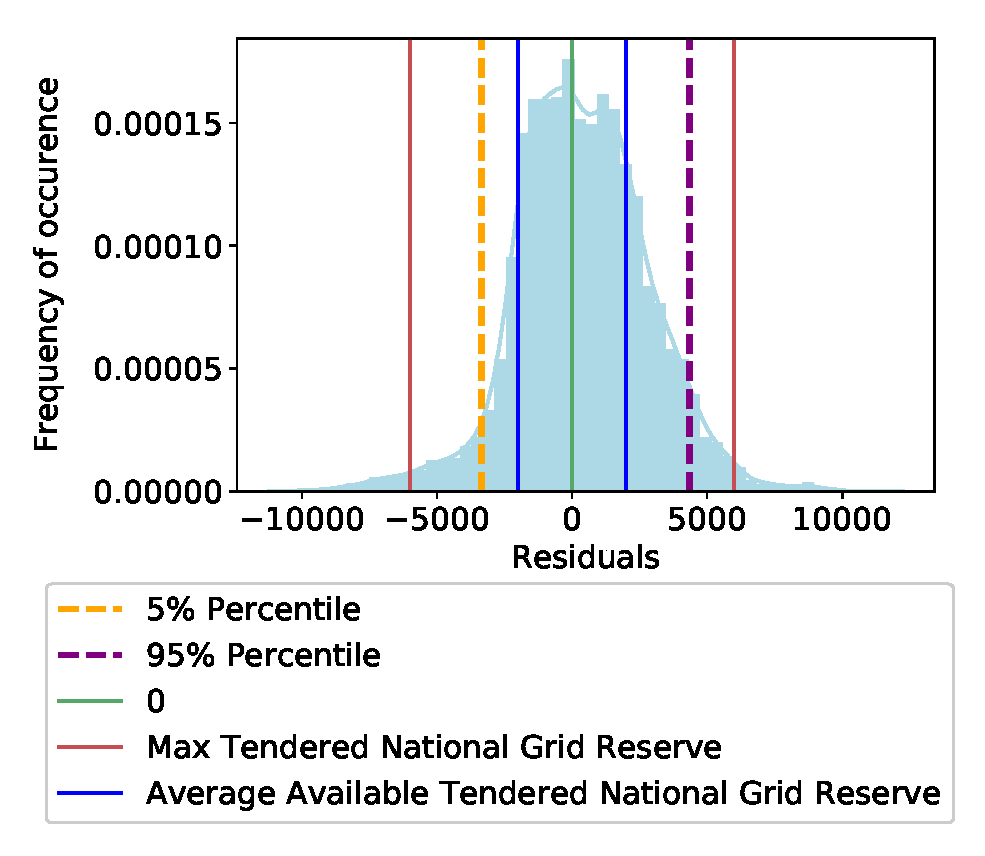
\includegraphics[width=0.65\columnwidth]{Chapter5/figures/market-forecasting/results/ExtraTreesRegressor_distribution_plot.eps}
	\caption{Best offline machine learning algorithm (Extra Trees Regressor) distribution.}
	\label{fig:best_offline_learning_day_distribution}
\end{figure}


%Figure \ref{fig:offline_fit_time_vs_mae} displays the amount of time it takes to train each of the models with respect to the mean absolute error. The error bars display the standard deviation between cross-validation runs. It can be seen that the models that take the longest to train are the machine learning methods, whereas the statistical methods take less time to train.


%\begin{figure}
%\centering
%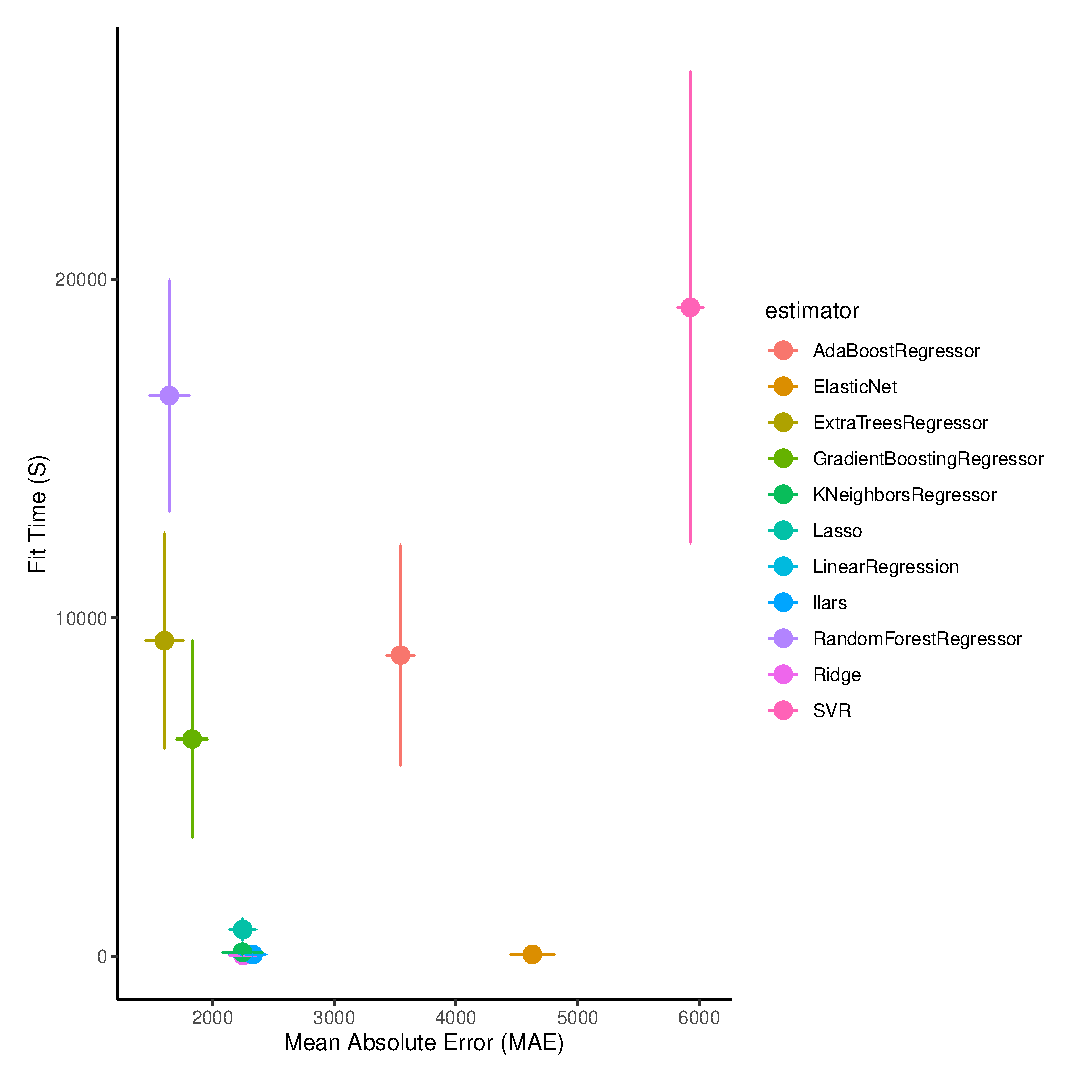
\includegraphics[width=\columnwidth,natwidth=500,natheight=500]{Chapter5/figures/market-forecasting/results/offline_fit_time_vs_mae.eps}
%\caption{Time taken to train the offline models versus mean absolute error. Error bars display standard deviation between points.}
%\label{fig:offline_fit_time_vs_mae}
%\end{figure}
%
%
%\begin{figure}
%\centering
%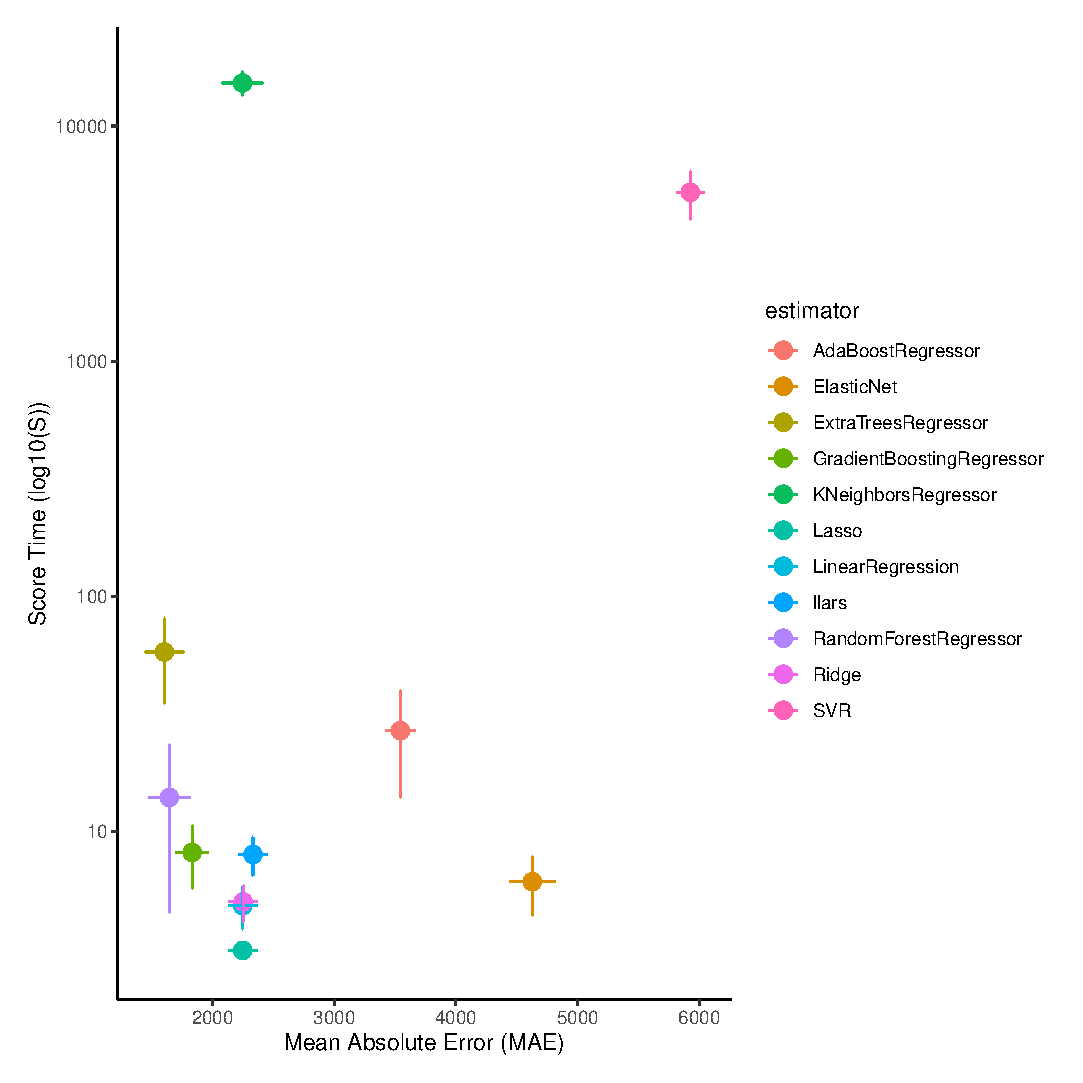
\includegraphics[width=\columnwidth,natwidth=500,natheight=500]{Chapter5/figures/market-forecasting/results/offline_score_time_vs_mae.eps}
%\caption{Time taken to score the offline models versus mean absolute error. Error bars display standard deviation between points.}
%\label{fig:offline_score_time_vs_mae}
%\end{figure}


Figures \ref{fig:offline_fit_time_vs_mae} and \ref{fig:offline_score_time_vs_mae} display the time taken to train the model and time taken to sample from the model versus the absolute error respectively for the offline algorithms. Multiple fits are trialled for each parameter type for each model. The error bars indicate the results of multiple cross-validations.

It can be seen from Figure \ref{fig:offline_fit_time_vs_mae} that the time to fit varies significantly between algorithms and parameter choices. The multilayer perceptron consistently takes a long time to fit, when compared to the other algorithms and performs relatively poorly in terms of MAE. There are many models, such as the random forest regressor, and extra trees regressors which perform well, however, take a long time to fit, especially when compared to the K-Nearest neighbours.

For a small deterioration in MAE it is possible to decrease the time it takes to train the model significantly. For example, by using the K-Nearest neighbours or support vector regression (SVR).

%\begin{figure}[h]
%\centering
%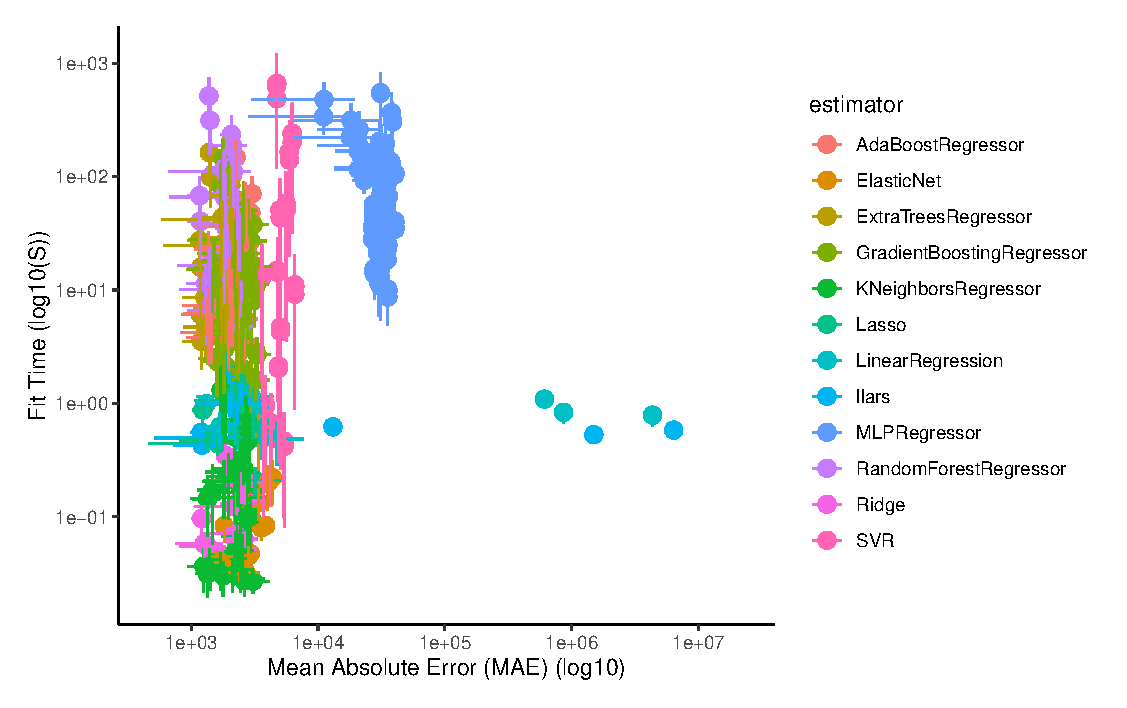
\includegraphics[width=\columnwidth,natwidth=500,natheight=500]{Chapter5/figures/market-forecasting/results/offline_fit_time_vs_mae_all_results.eps}
%\caption{Time taken to train the offline models versus mean absolute error. Error bars display standard deviation between points.}
%\label{fig:offline_fit_time_vs_mae}
%\end{figure}

\begin{figure}[H]
	\centering
	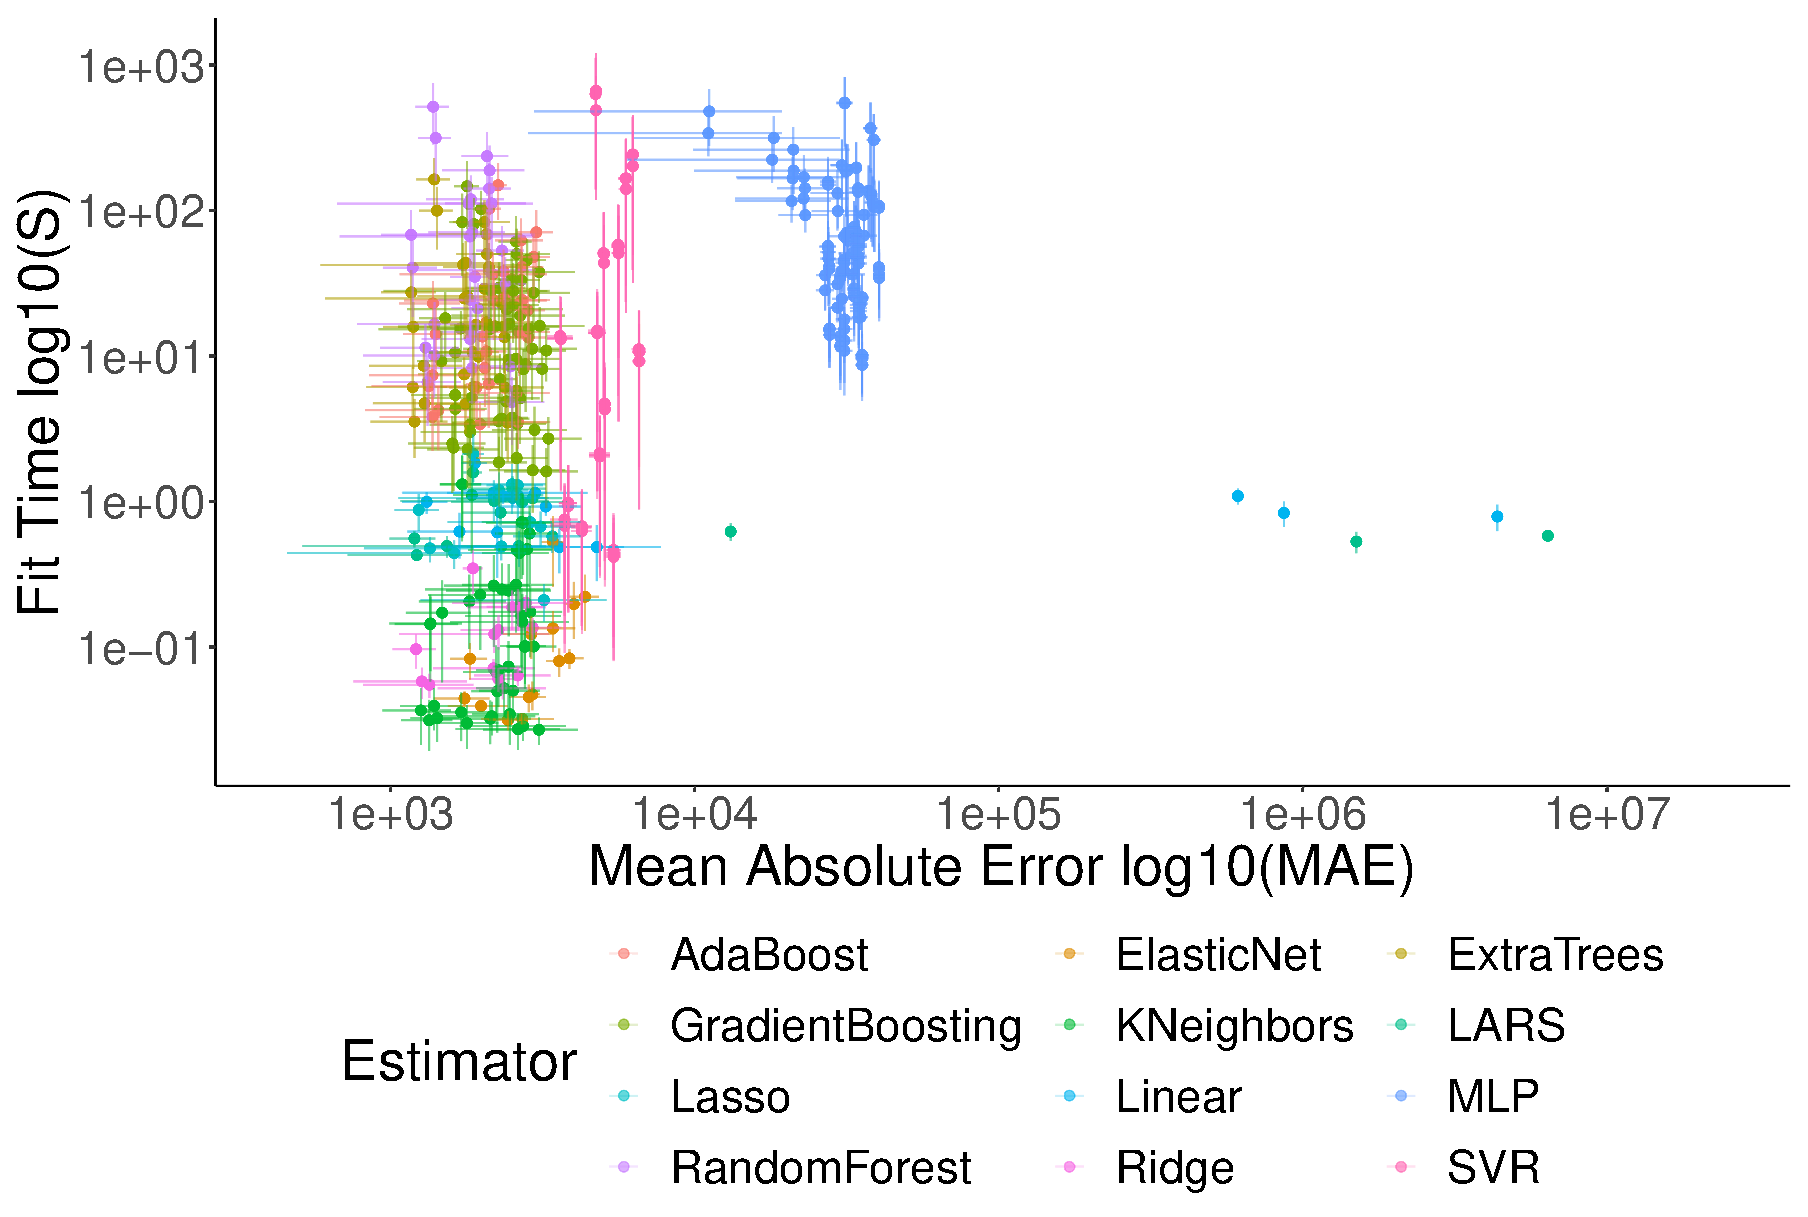
\includegraphics[width=0.65\columnwidth]{Chapter5/figures/market-forecasting/results/offline_fit_time_vs_mae_all_results_opaque.eps}
	\caption{Time taken to train the offline models versus mean absolute error. Error bars display standard deviation between points.}
	\label{fig:offline_fit_time_vs_mae}
\end{figure}


The scoring time, displayed in Figure \ref{fig:offline_score_time_vs_mae}, also displays a large variation between model types. For instance, the MLP regressor takes a shorter time to sample predictions when compared to the K-Neighbors algorithm and support vector regression. It is possible to have a cluster of algorithms with low sample times and low mean absolute errors. However, often a trade-off is required, with a fast prediction time requiring a longer training time and vice-versa. 



\begin{figure}[H]
	\centering
	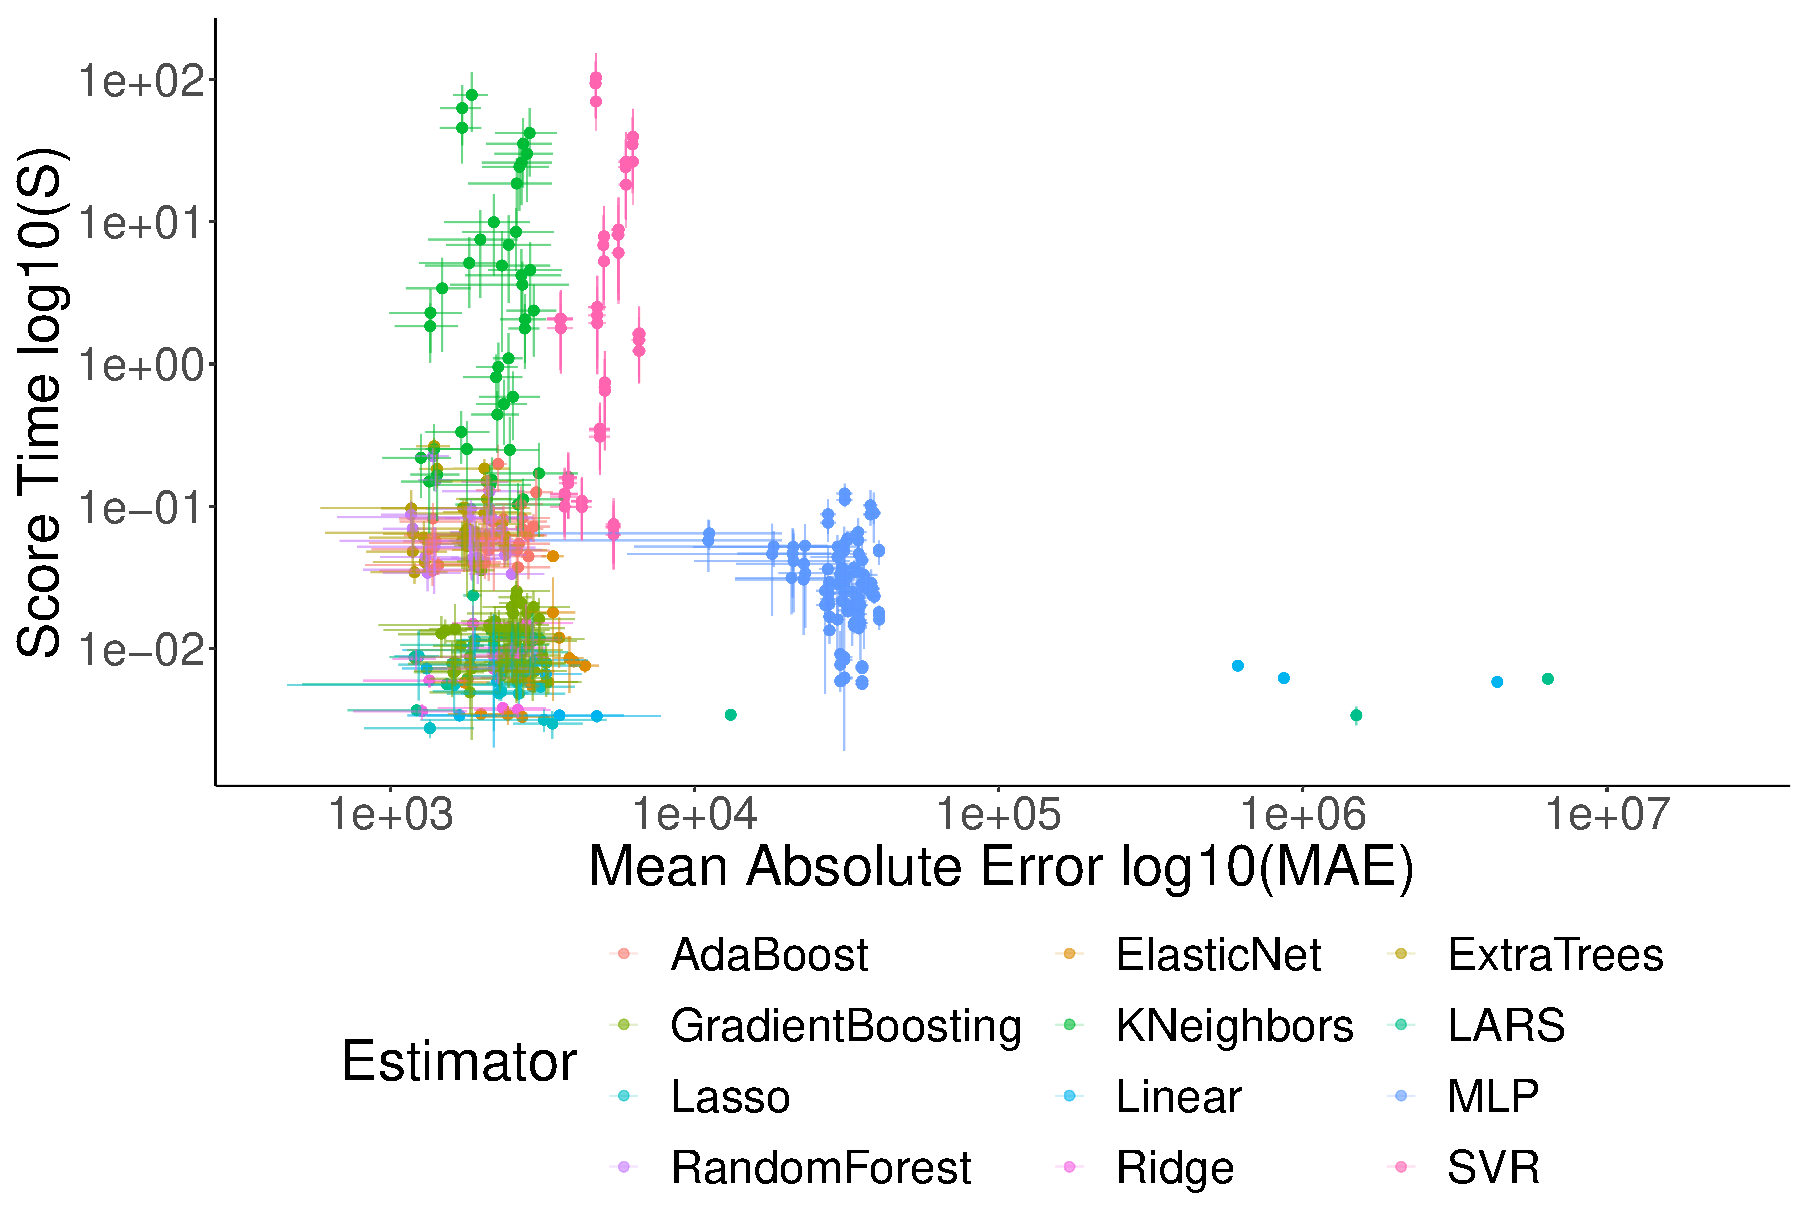
\includegraphics[width=0.65\columnwidth]{Chapter5/figures/market-forecasting/results/offline_score_time_vs_mae_all_results_opaque.eps}
	\caption{Time taken to score the offline models versus mean absolute error. Error bars display standard deviation between points.}
	\label{fig:offline_score_time_vs_mae}
\end{figure}









\subsubsection{Online Machine Learning}

\begin{figure}
	\centering
	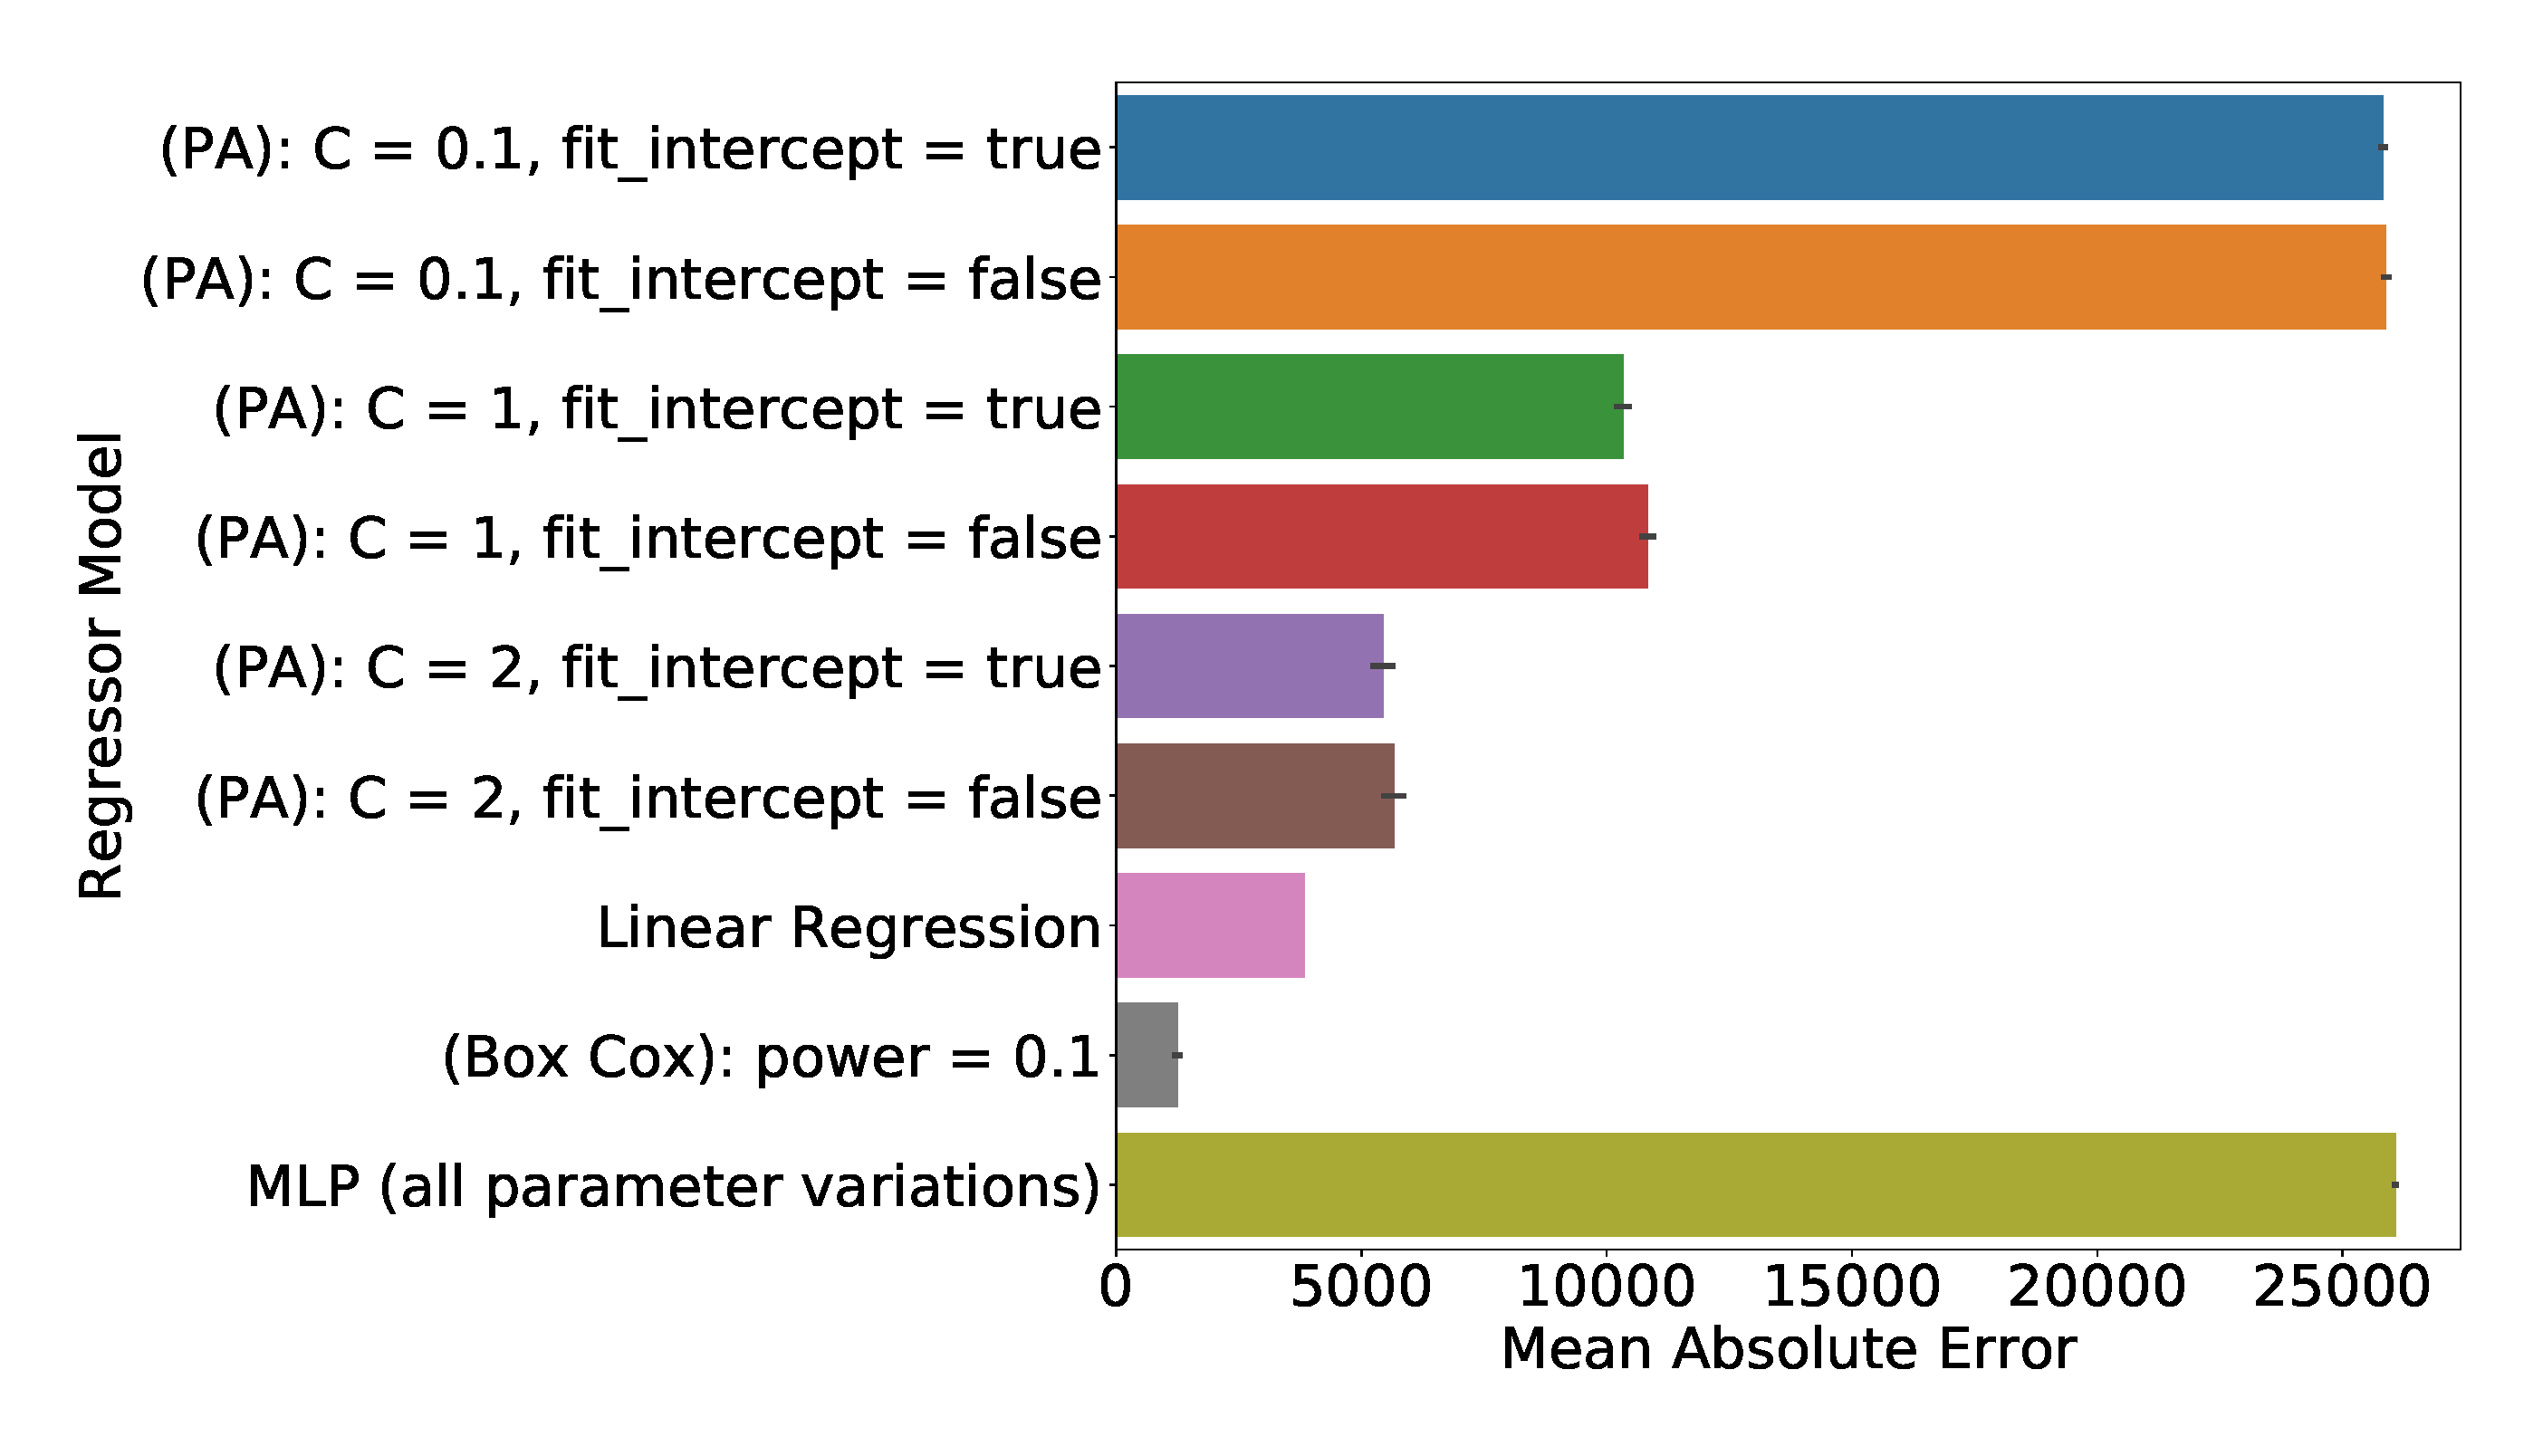
\includegraphics[width=0.65\columnwidth]{Chapter5/figures/market-forecasting/results/online_model_mae_barplot.eps}
	\caption{Comparison of mean absolute errors (MAE) for different online regressor models. MLP results for all parameters are shown in a single barchart due to the very similar MAEs for the differing hyperparameters.}
	\label{fig:online_model_mae_barplot}
\end{figure}



To see if we can improve on the predictions, we utilize an online machine learning approach. If we are successful, we should be able to reduce the national grid reserves, reducing cost and emissions.


Figure \ref{fig:online_model_mae_barplot} displays the comparison of mean absolute errors for the different trialled online regressor models. To produce this graph, we showed various hyperparameter trials. Where the hyperparameters had the same results, we removed them. For the multilayer perceptron (MLP), we aggregated all hyperparameters, due to the similar nature of the predictions.

It can be seen that the best performing model was the Box-Cox regressor, with an MAE of 1100. This is an improvement of over 30\% on the best offline model. The other models perform less well. However, it can be seen that the linear regression model improves significantly for the online case when compared to the offline case. The passive aggressive (PA) model improve significantly with the varying parameters, and the MLP performs poorly in all cases.



Figure \ref{fig:best_online_learning_day_distribution} displays the best online model. We can see a significant improvement over the best online model distribution, shown in Figure \ref{fig:best_offline_learning_day_distribution}. We remain within the max tendered national grid reserve for 98.9\% of the time, and the average available tendered national grid reserve is close to the 5\% and 95\% percentiles.



\begin{figure}
	\centering
	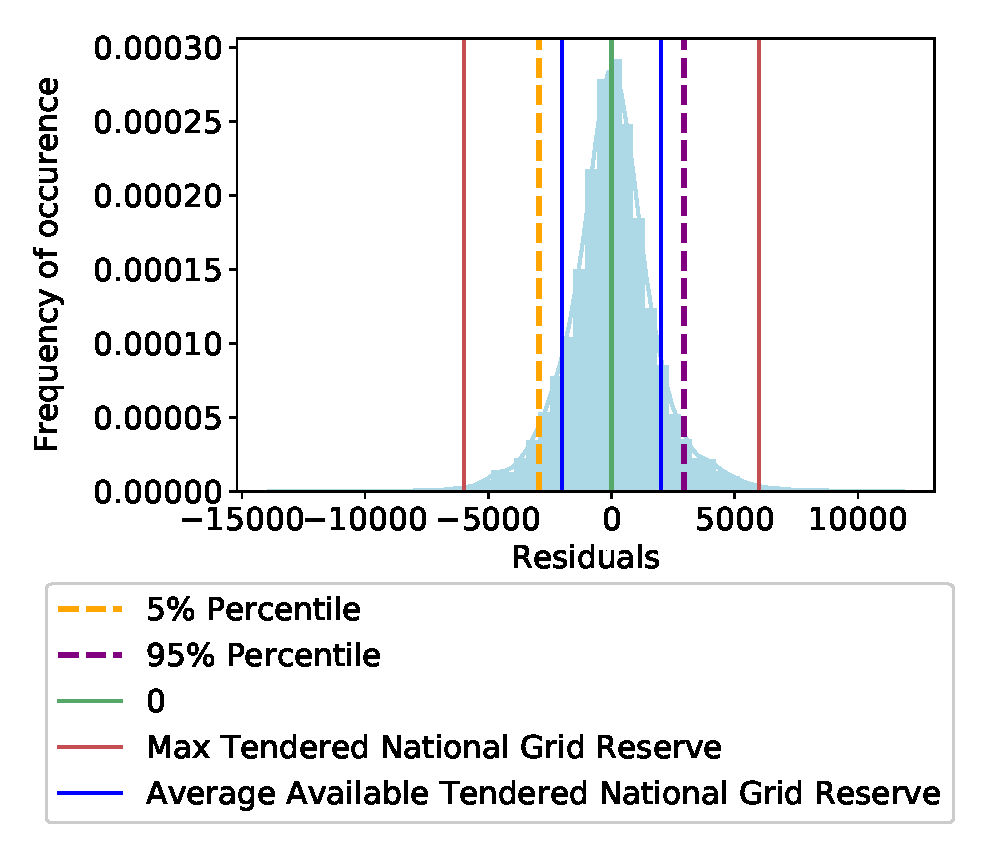
\includegraphics[width=0.6\columnwidth]{Chapter5/figures/market-forecasting/results/online_learning_dists-power-0.1.eps}
	\caption{Best online model (Box-Cox Regressor) distribution.}
	\label{fig:best_online_learning_day_distribution}
\end{figure}

Figure \ref{fig:bad_online_learning_day_distribution} displays the residuals for a model with poor predictive ability, the passive aggressive regressor. It displays a large period of time of prediction errors at -20,000MWh, and often falls outside of the national grid reserve. These results demonstrate the importance of trying a multitude of different models and parameters to improve prediction accuracy.

\begin{figure}
	\centering
	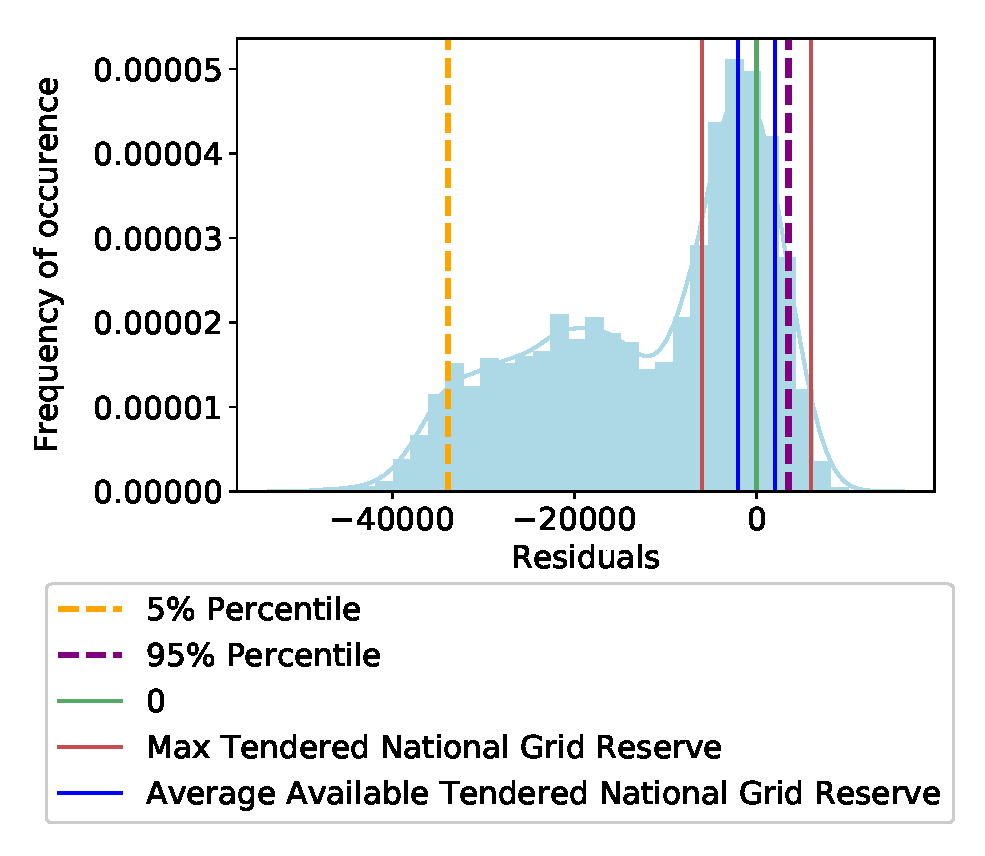
\includegraphics[width=0.6\columnwidth]{Chapter5/figures/market-forecasting/results/online_learning_dists-C-0.1-fit_intercept-true-max_iter-1000-shuffle-false-tol-001.eps}
	\caption{Online machine learning algorithm distribution. (Passive Aggressive Regressor (C=0.1, fit intercept = true, maximum iterations = 1000, shuffle = false, tolerance = 0.001), chosen as it was the worst result for the passive aggressive model.}
	\label{fig:bad_online_learning_day_distribution}
\end{figure}


Figure \ref{fig:both_actual_predicted} displays a comparison between the actual electricity consumption compared to the predictions. It can be seen that the Box-Cox model better predicts the actual electricity demand in most cases when compared to the best offline model, the Extra Trees regressor. The Extra Trees regressor often overestimates the demand, particularly during weekdays. Whilst the Box-Cox regressor more closely matches the actual results. During the weekend (between the hours of 120 and 168), the Extra Trees regressor performs better, particularly on the Saturday (between hours of 144 and 168). 


\begin{figure}
	\centering
	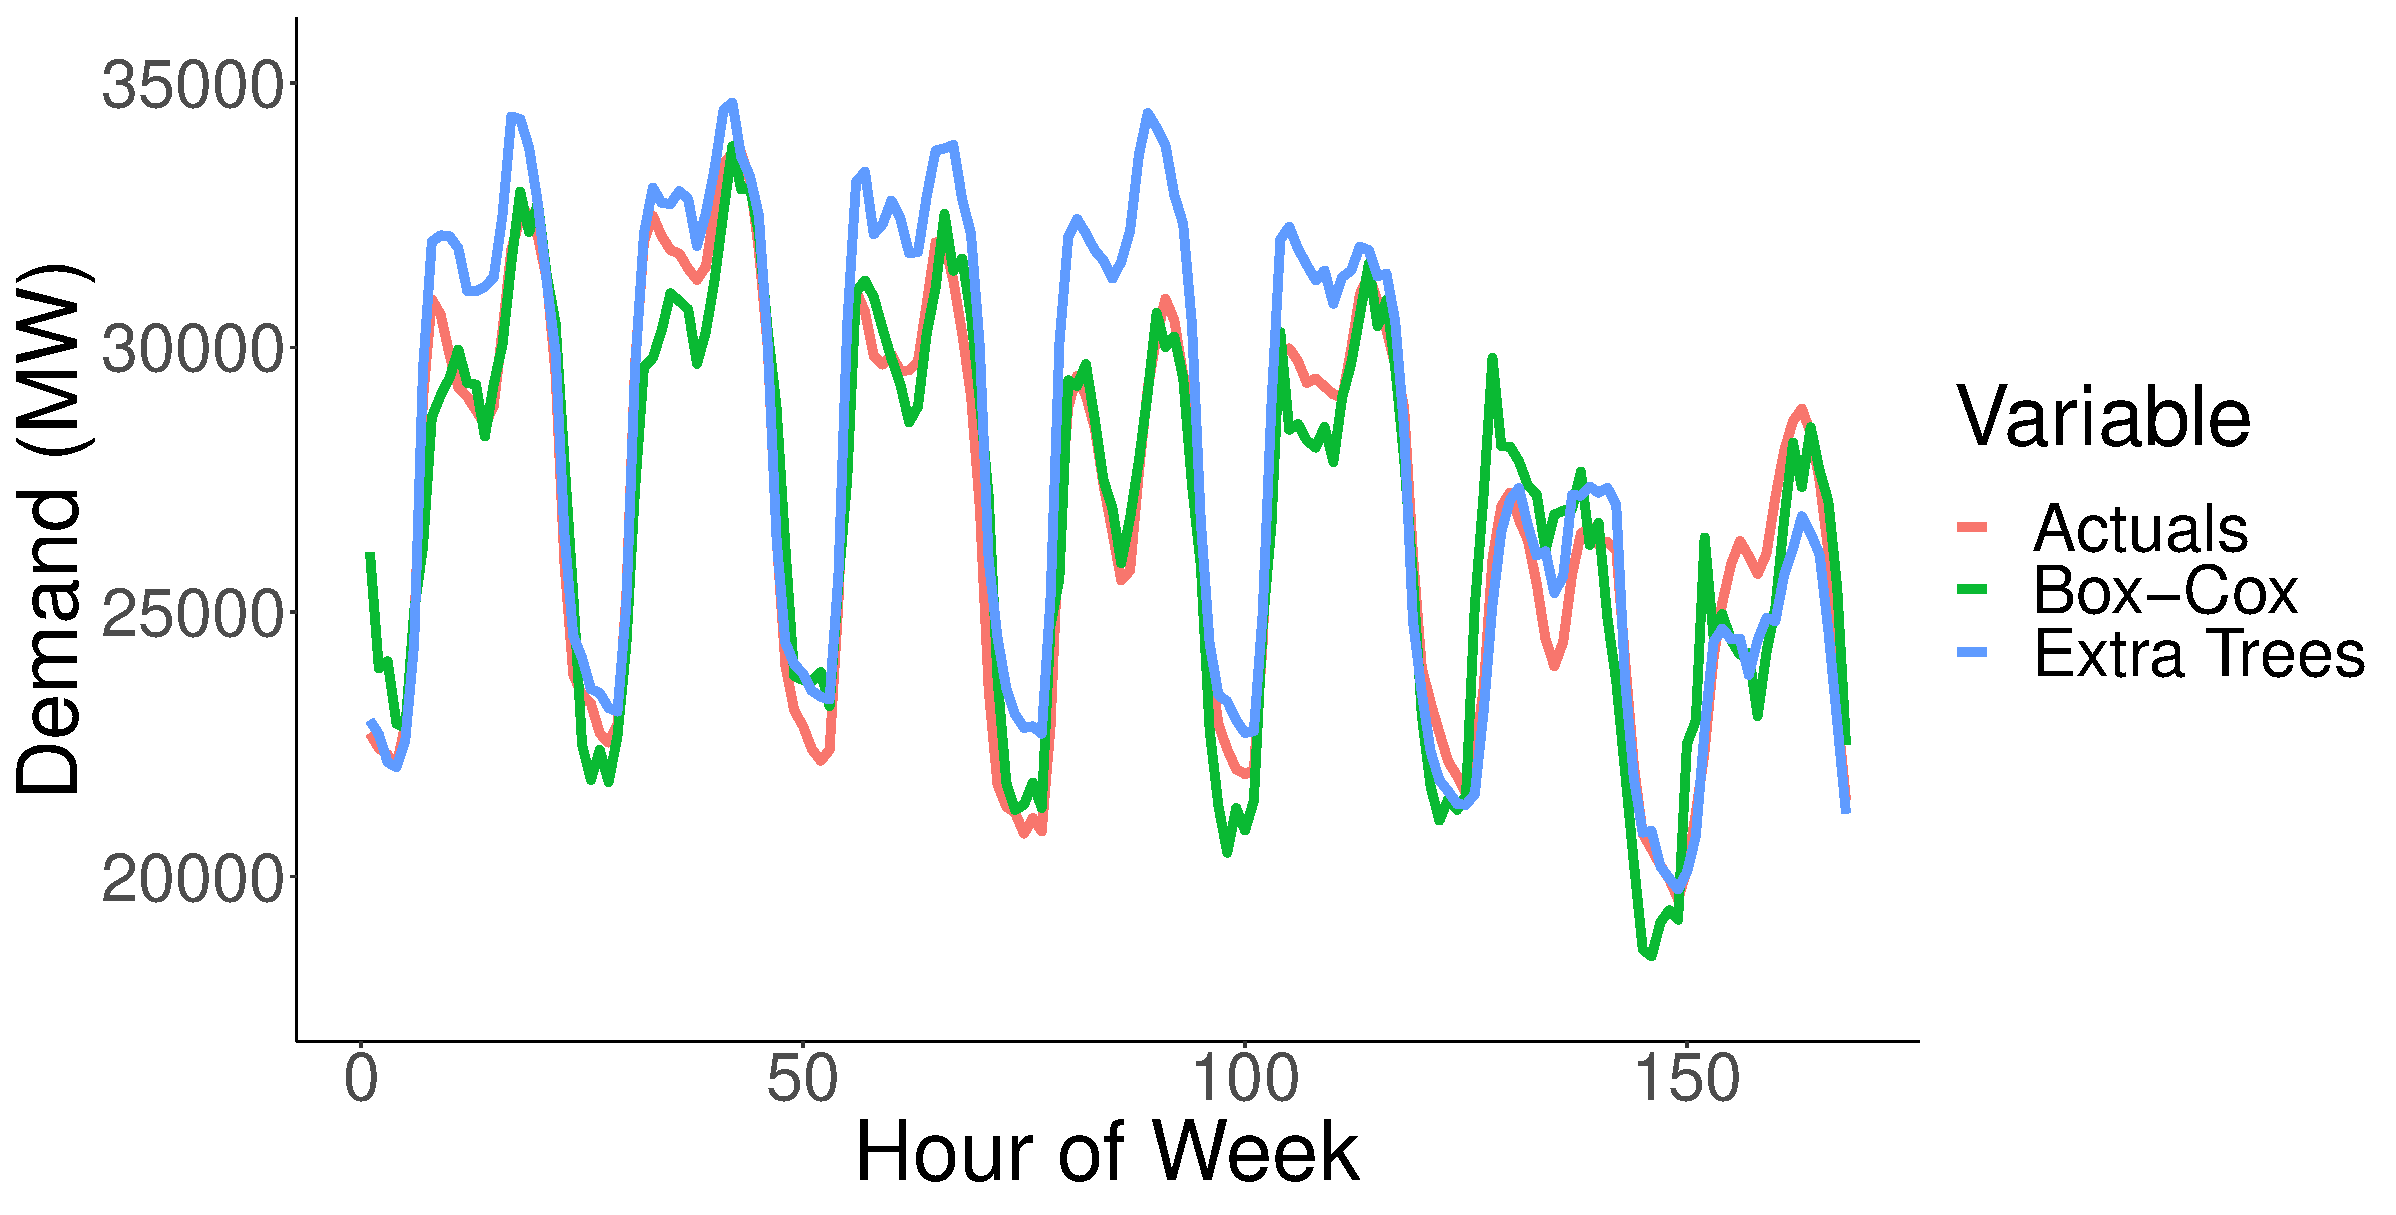
\includegraphics[width=0.6\columnwidth]{Chapter5/figures/market-forecasting/results/both_actual_predicted.eps}
	\caption{Best offline model compared to the best online model over a one week period.}
	\label{fig:both_actual_predicted}
\end{figure}

Figures \ref{fig:online_test_vs_mae} and \ref{fig:online_train_vs_mae} display the mean absolute error versus test and training time respectively. In these graphs, a selection of models and parameter combinations are chosen. 

Clear clusters can be seen between different types of models and parameter types. With the passive aggressive (PA) model performing the slowest for both training and testing. Different parameter combinations show different results in terms of mean absolute error.

The best performing model is the Box-Cox model, which is also the fastest to both train and test. The linear regression, which performs worse in terms of predictive performance, is as quick to train and test as the Box-Cox model. Additionally, the multilayer perceptron (MLP) is relatively quick to train and test when compared to the PA models. 

It is noted that when compared to the offline models, the training time is a good indicator to the testing time. In other words, models that are fast to train are also fast to test and vice-versa.




\begin{figure}
	\centering
	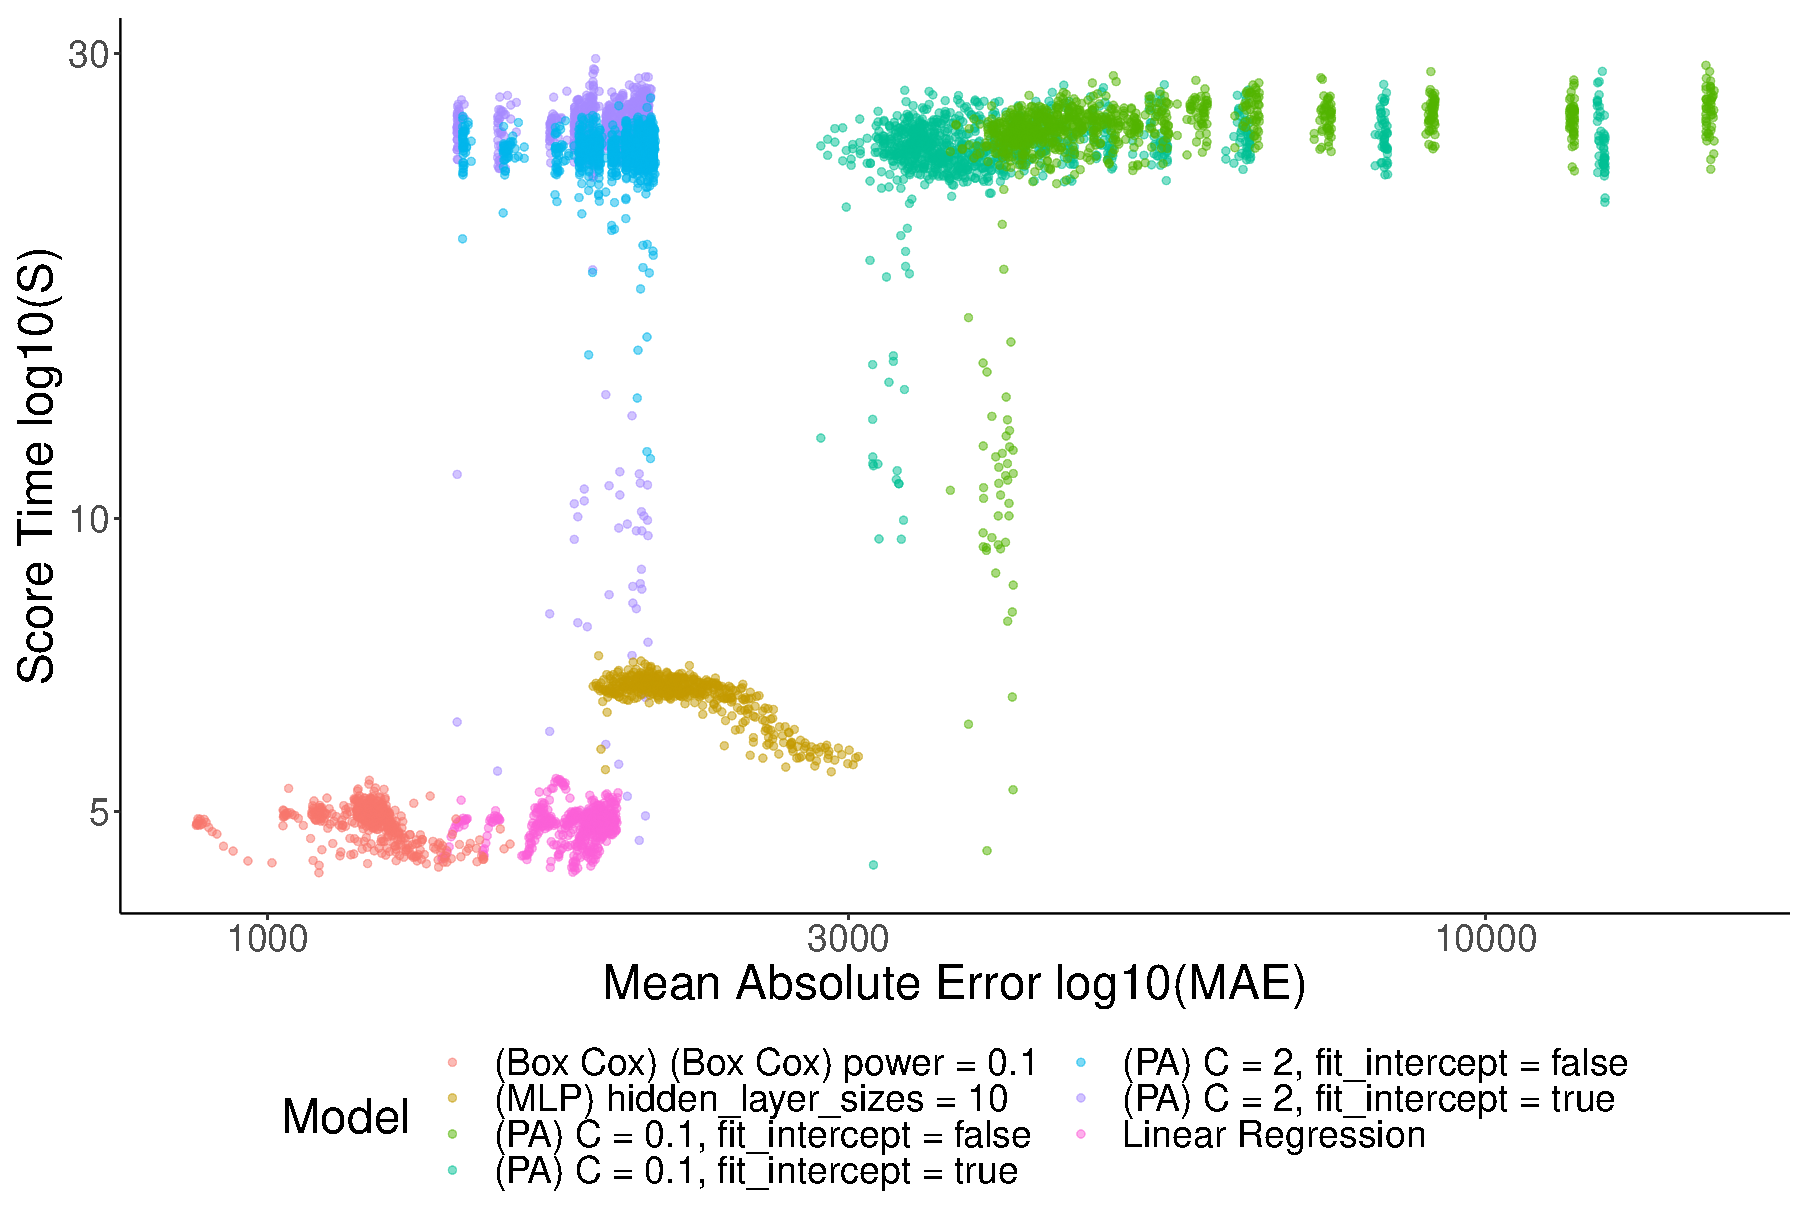
\includegraphics[width=0.6\columnwidth]{Chapter5/figures/market-forecasting/results/online_testing_time_vs_mae_all_results_opaque.eps}
	\caption{Time taken to test the online models versus mean absolute error.}
	\label{fig:online_test_vs_mae}
\end{figure}

\begin{figure}
	\centering
	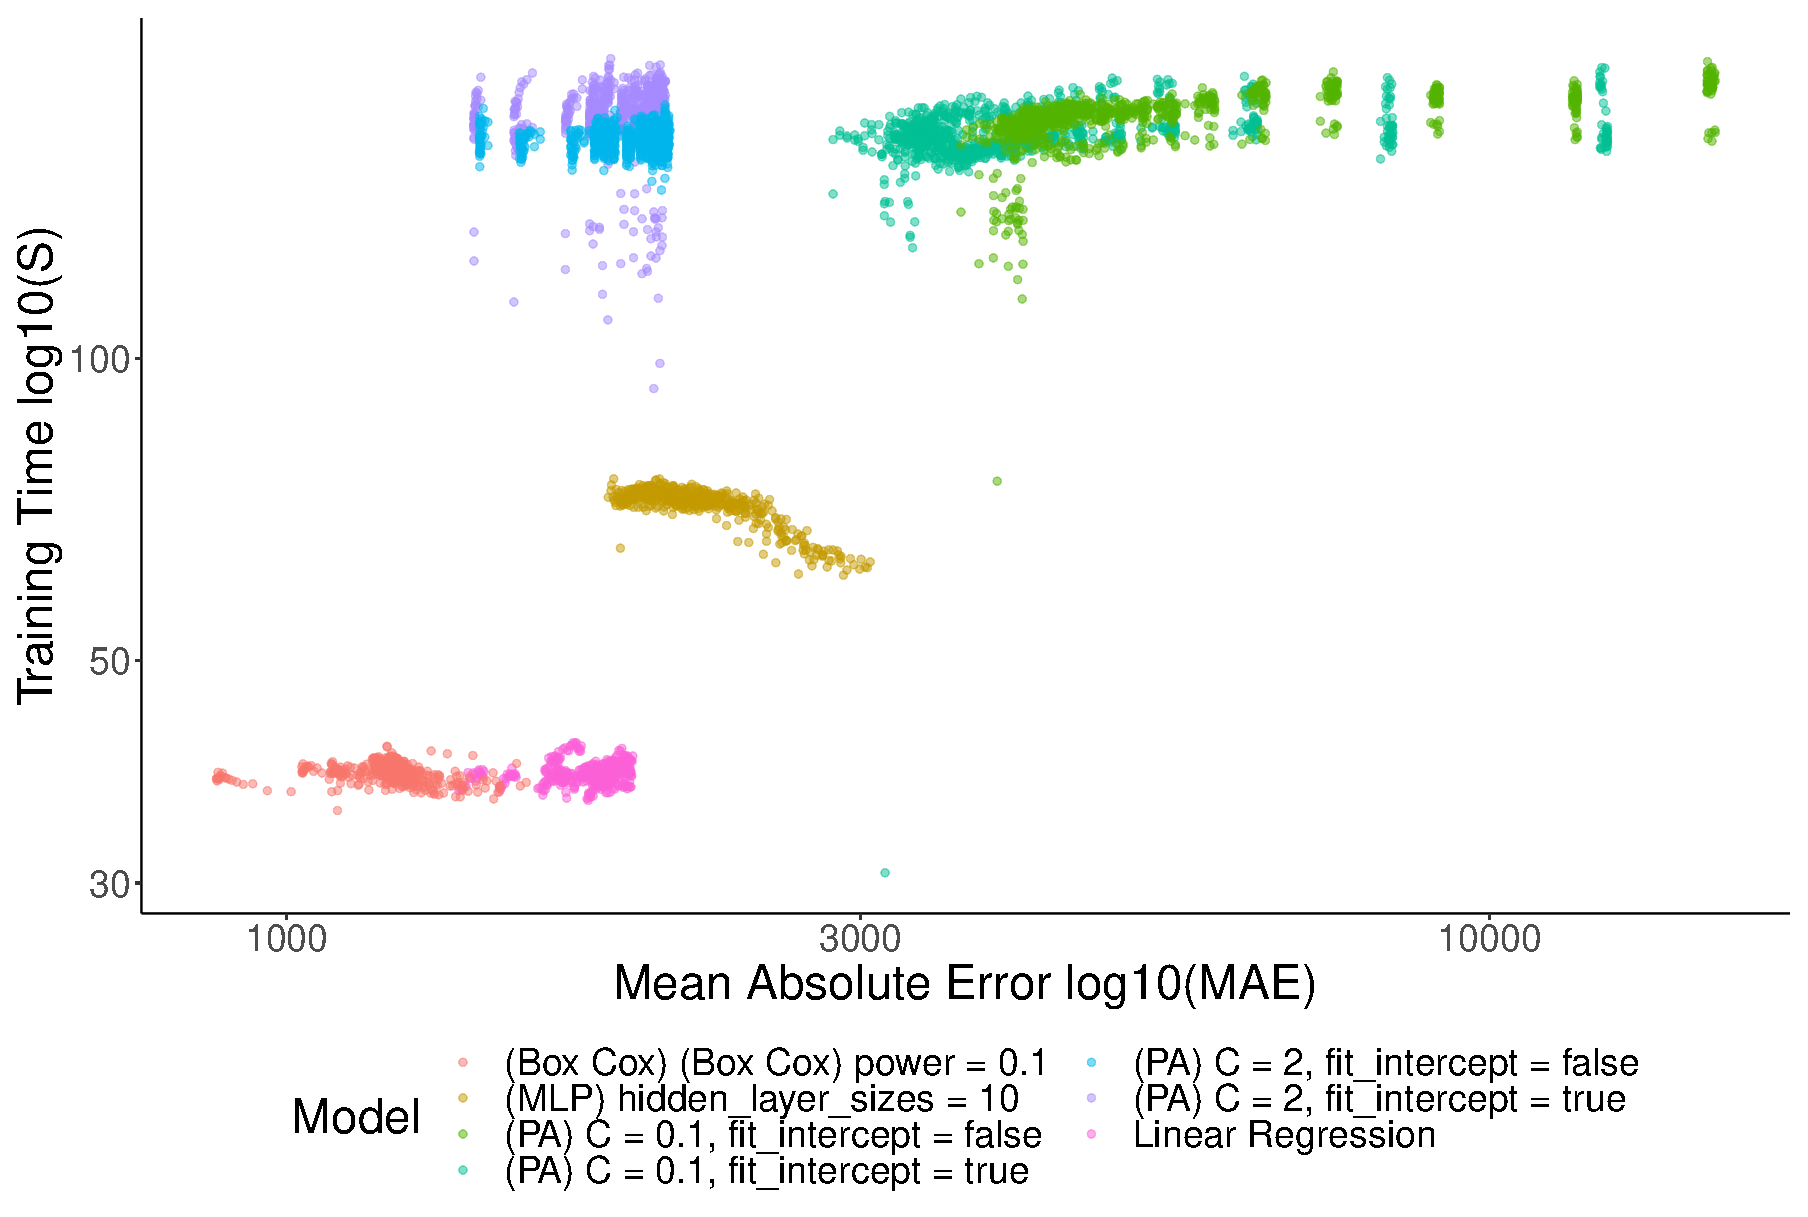
\includegraphics[width=0.6\columnwidth]{Chapter5/figures/market-forecasting/results/online_training_time_vs_mae_all_results_opaque.eps}
	\caption{Time taken to train the online models versus mean absolute error.}
	\label{fig:online_train_vs_mae}
\end{figure}








\subsection{Scenario Comparison}

In this Section we explore the effect of these residuals on investments made and the electricity generation mix.  To generate these graphs, we perturbed the exogenous demand in ElecSim by sampling from the best-fitting distributions for the respective residuals of each of the online methods. We did this for all of the online learning algorithms displayed in Figure \ref{fig:online_model_mae_barplot}. We let the simulation run for 17 years from 2018 to 2035. 

Running this simulation enabled us to see the effect on carbon emissions on the electricity grid over a long time period. For instance, does underestimating electricity demand mean that peaker power plants, such as reciprocal gas engines, are over utilized when other, less polluting power plants could be used?



\subsubsection{Mean Contributed Energy Generation}


\begin{figure*}
	\centering
	\begin{subfigure}{0.3\textwidth}
		%\centering
		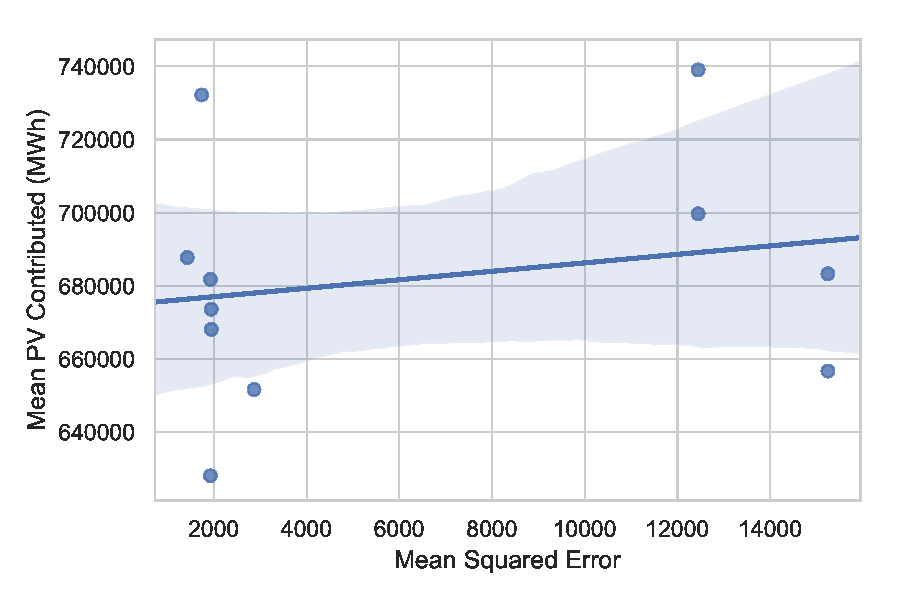
\includegraphics[width=\columnwidth]{Chapter5/figures/market-forecasting/results/elecsim_results/results_2/contributed_PV_mean_output}
		\caption{Photovoltaic output.}
		\label{fig:contributed_PV_mean_output}
	\end{subfigure}
	\hfil
	\begin{subfigure}{0.3\textwidth}  
		%\centering
		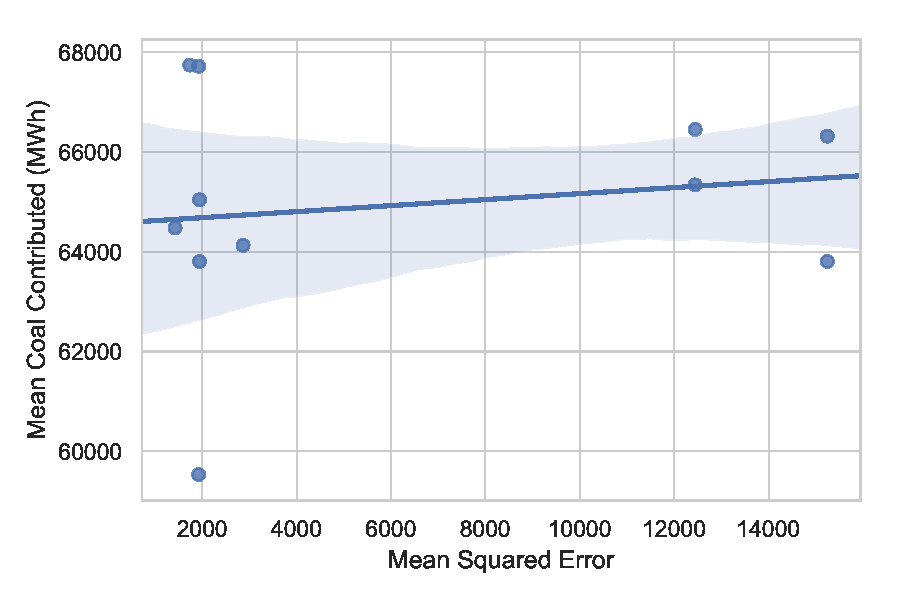
\includegraphics[width=\columnwidth]{Chapter5/figures/market-forecasting/results/elecsim_results/results_2/contributed_Coal_mean_output.eps}
		\caption{Coal output.}
		\label{fig:contributed_Coal_mean_output}
	\end{subfigure}
	\hfil
	%\vskip\baselineskip
	\begin{subfigure}{0.3\textwidth}   
		%\centering
		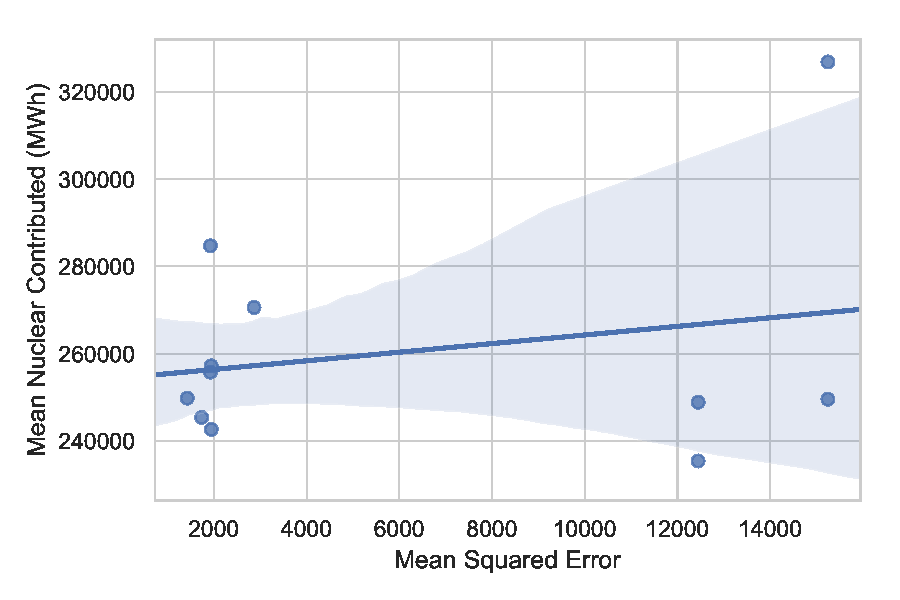
\includegraphics[width=\columnwidth]{Chapter5/figures/market-forecasting/results/elecsim_results/results_2/contributed_Nuclear_mean_output.eps}
		\caption{Nuclear output.}
		\label{fig:contributed_Nuclear_mean_output}
	\end{subfigure}
	%\quad
	\medskip
	\begin{subfigure}{0.3\textwidth}   
		%\centering
		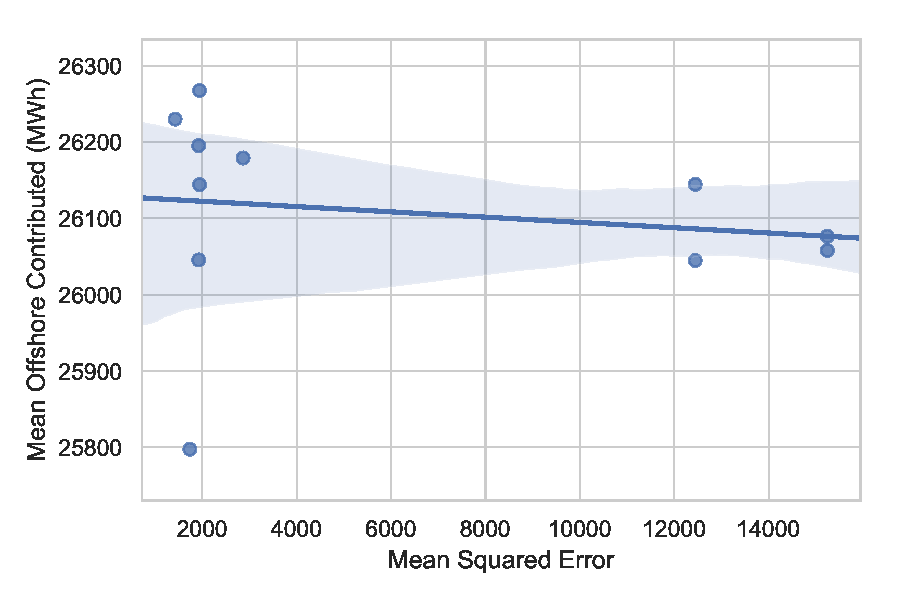
\includegraphics[width=\columnwidth]{Chapter5/figures/market-forecasting/results/elecsim_results/results_2/contributed_Offshore_mean_output.eps}
		\caption{Offshore output.}
		\label{fig:contributed_Offshore_mean_output.eps}
	\end{subfigure}
	\hfil
	\begin{subfigure}{0.3\textwidth}   
		%\centering
		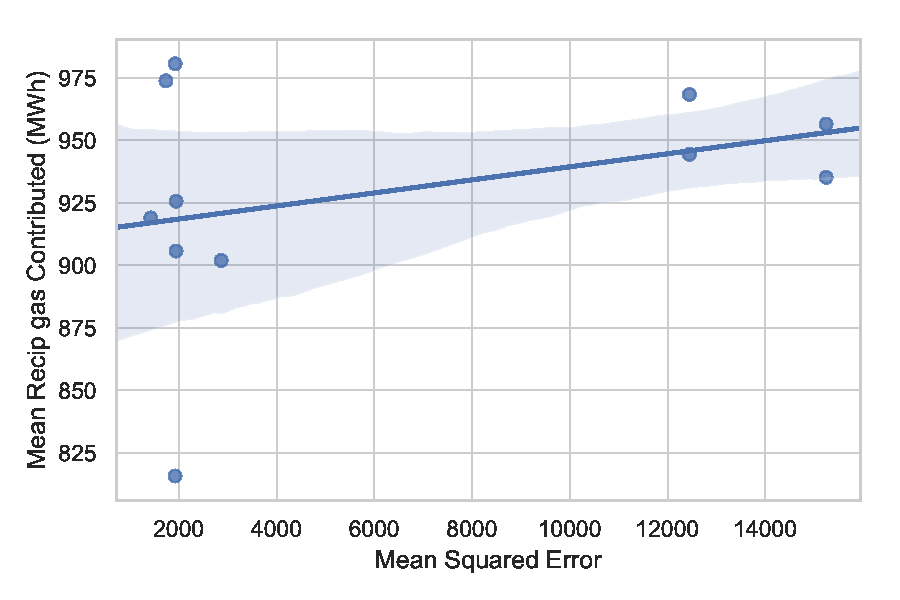
\includegraphics[width=1\columnwidth]{Chapter5/figures/market-forecasting/results/elecsim_results/results_2/contributed_Recip_gas_mean_output.eps}
		\caption{Reciprocal gas engine output.}
		\label{fig:contributed_Recip_gas_mean_output}
	\end{subfigure}
	\label{fig:pv_coal_nuclear_offshore_outputs}
	\caption{Mean outputs of various technologies vs. mean absolute error from 2018 to 2035 in ElecSim.}
\end{figure*}

In this Section we display the mean electricity mix contributed by different electricity sources over the years 2018 to 2035. 

Figure \ref{fig:contributed_PV_mean_output} displays the mean photovoltaic (PV) contributed between 2018 and 2035 vs. mean absolute error of the various online regressor models displayed in Figure \ref{fig:online_model_mae_barplot}. A positive correlation can be seen with PV contributed and mean absolute error. This is similar for coal and nuclear output, shown in Figures \ref{fig:contributed_Coal_mean_output} and \ref{fig:contributed_Nuclear_mean_output} respectively. However, as shown by Figure \ref{fig:contributed_Offshore_mean_output.eps}, offshore wind reduces with mean absolute error. Figure \ref{fig:contributed_Recip_gas_mean_output} displays the mean reciprocal gas engine output vs mean absolute error between the same time period. Output for the reciprocal gas engine also increases with mean absolute error.

The reciprocal gas engine was expected to increase with times of high error. This is because, traditionally, reciprocal gas engines are peaker power plants. Peaker power plants provide power at times of peak demand, which cannot be covered by other plants due to them being at their maximum capacity level or out of service. It may also be the case, that with higher proportions of intermittent technologies, there is a larger need for these peaker power plants to fill in for times where there is a deficit in wind speed and solar irradiance.

It is hypothesized that coal and nuclear output increase to cover the predicted increased demands of the service. As these generation types are dispatchable, meaning operators can choose when they generate electricity, they are more likely to be used in times of higher predicted demand.

Photovoltaics may be used more with higher errors due to the times at which the errors were greatest. For example, during the day, where demand is higher, as is solar irradiance.





%\begin{subfigure}
%%\centering
%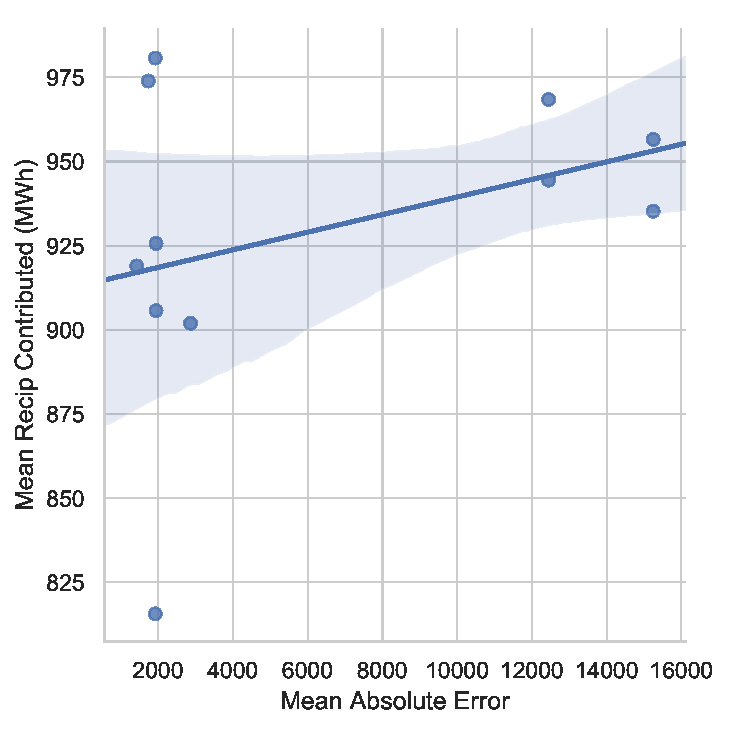
\includegraphics[width=0.3\textwidth]{Chapter5/figures/market-forecasting/results/elecsim_results/contributed_Recip_gas_mean_output.eps}
%\caption{Mean reciprocal gas engine output vs. mean absolute error from 2018 to 2035 in ElecSim.}
%\label{fig:contributed_Recip_gas_mean_output}
%\end{subfigure}

%
%
%\begin{figure}
%\centering
%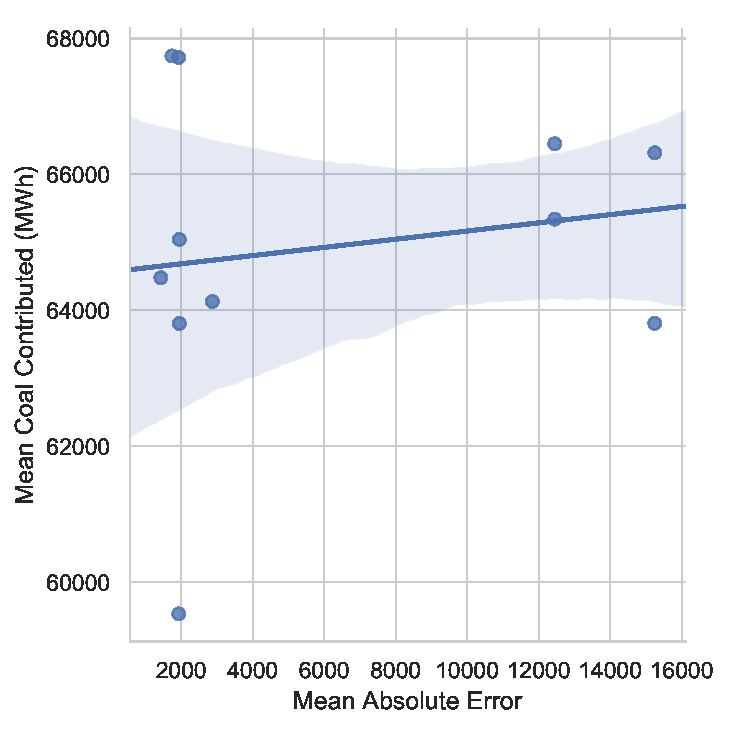
\includegraphics[width=\columnwidth]{Chapter5/figures/market-forecasting/results/elecsim_results/contributed_Coal_mean_output.eps}
%\caption{Mean coal output vs. mean absolute error from 2018 to 2035 in ElecSim.}
%\label{fig:contributed_Coal_mean_output}
%\end{figure}
%
%
%\begin{figure}
%\centering
%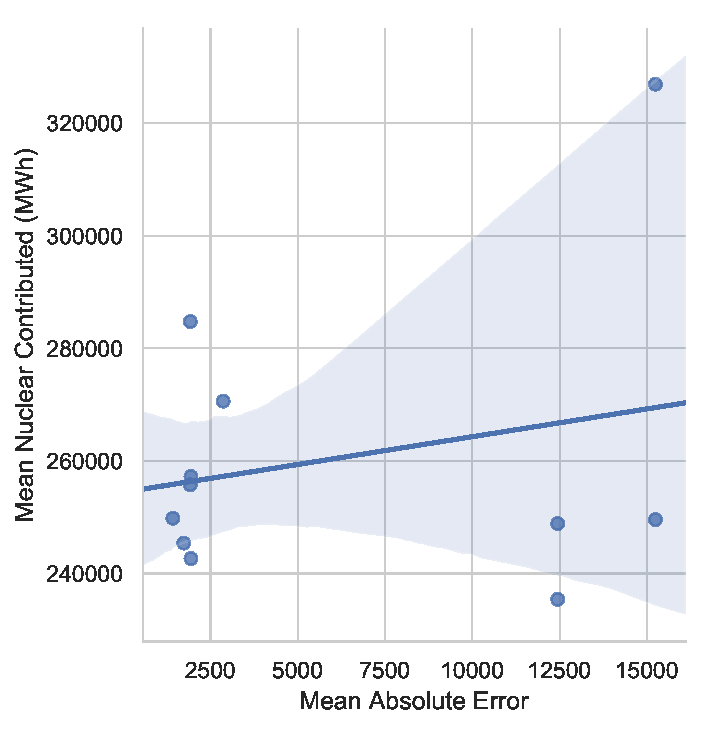
\includegraphics[width=\columnwidth]{Chapter5/figures/market-forecasting/results/elecsim_results/contributed_Nuclear_mean_output.eps}
%\caption{Mean nuclear output vs. mean absolute error from 2018 to 2035 in ElecSim.}
%\label{fig:contributed_Nuclear_mean_output}
%\end{figure}
%
%
%\begin{figure}
%\centering
%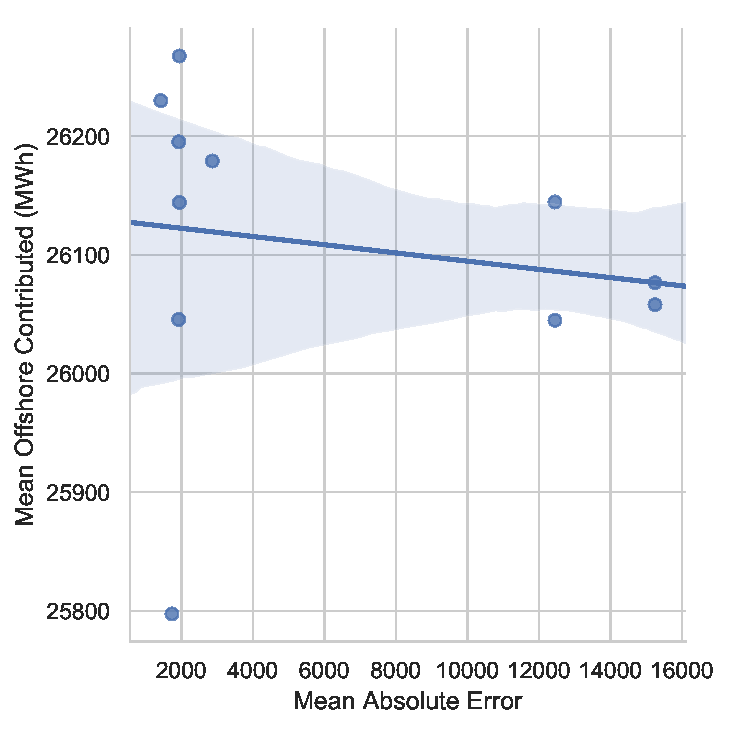
\includegraphics[width=\columnwidth]{Chapter5/figures/market-forecasting/results/elecsim_results/contributed_Offshore_mean_output.eps}
%\caption{Mean offshore output vs. mean absolute error from 2018 to 2035 in ElecSim.}
%\label{fig:contributed_Offshore_mean_output.eps}
%\end{figure}

%\begin{figure}
%\centering
%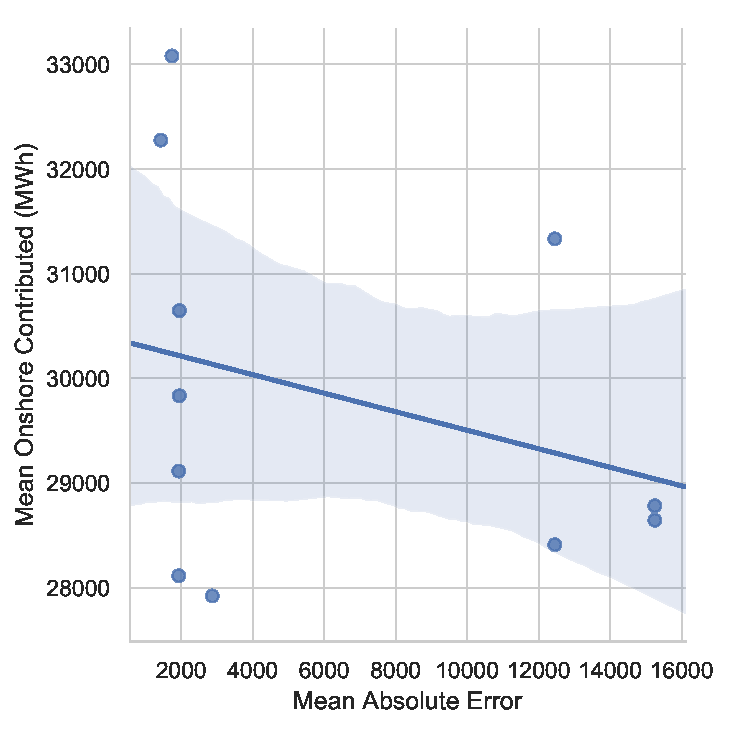
\includegraphics[width=\columnwidth]{Chapter5/figures/market-forecasting/results/elecsim_results/contributed_Onshore_mean_output.eps}
%\caption{Mean onshore output vs. mean absolute error from 2018 to 2035 in ElecSim.}
%\label{fig:contributed_Onshore_mean_output.eps}
%\end{figure}


%\begin{figure}
%\centering
%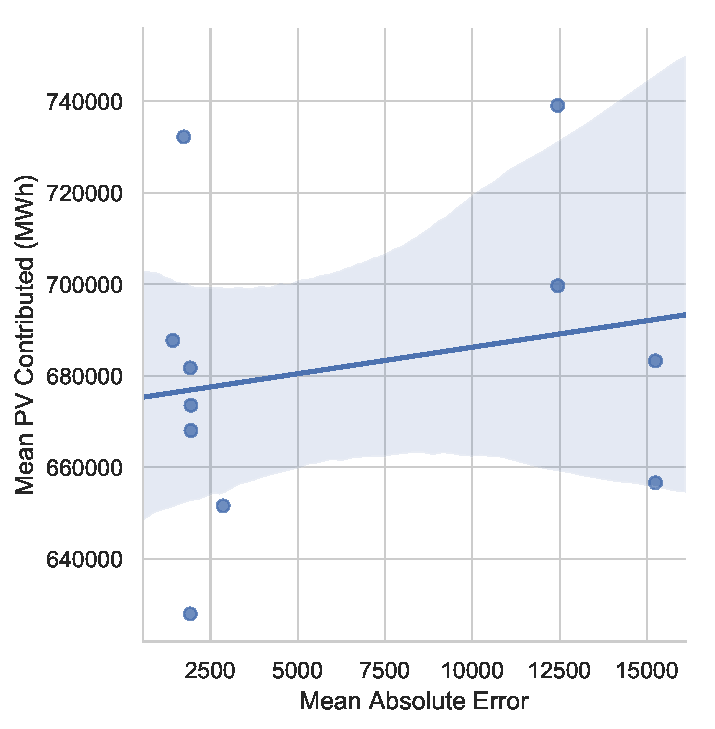
\includegraphics[width=\columnwidth]{Chapter5/figures/market-forecasting/results/elecsim_results/contributed_PV_mean_output}
%\caption{Mean photovoltaic output vs. mean absolute error from 2018 to 2035 in ElecSim.}
%\label{fig:contributed_PV_mean_output}
%\end{figure}








\subsubsection{Total Energy Generation}



In this Section, we detail the difference in total technologies invested in over the time period between 2018 to 2035, as predicted by ElecSim.

CCGT, onshore, and reciprocal gas engines are invested in less over the time period, as shown by Figures \ref{fig:total_CCGT_mean_output}, \ref{fig:total_Offshore_mean_output}, \ref{fig:total_Recip_gas_mean_output.eps} respectively. While coal, offshore, nuclear and photovoltaics all exhibit increasing investments.

It is hypothesized that coal and nuclear increase in investment due to their dispatchable nature. While onshore, non-dispatchable by nature, become a less attractive investment when compared to the other technologies.

CCGT and reciprocal gas engines may have decreased in capacity over this time, due to the increase in coal. This could be because of the large consistent errors in prediction accuracy that meant that reciprocal gas engines were perceived to be less valuable.


\begin{figure*}
	\centering
	\begin{subfigure}{0.3\textwidth}
		%\centering
		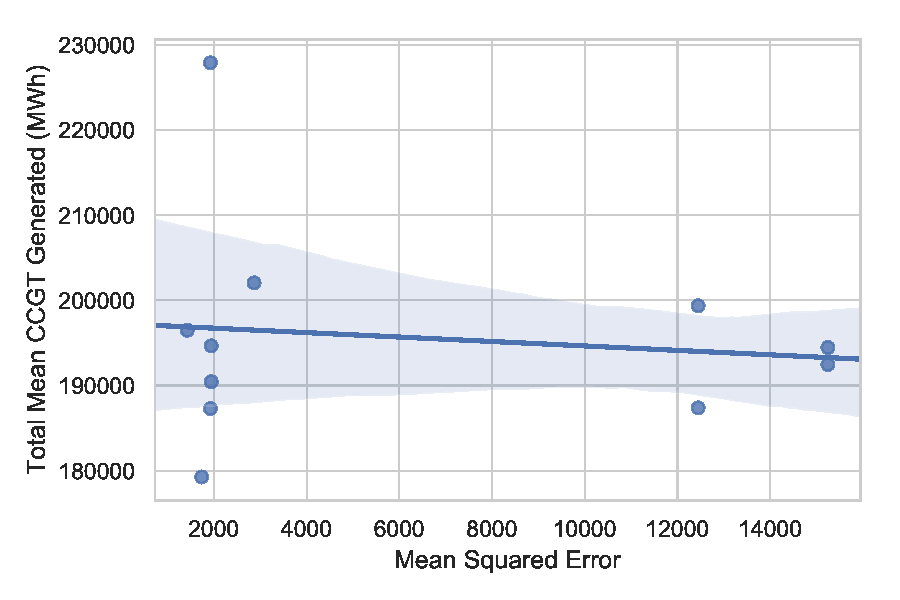
\includegraphics[width=\columnwidth]{Chapter5/figures/market-forecasting/results/elecsim_results/results_2/total_CCGT_mean_output.eps}
		\caption{Total CCGT.}
		\label{fig:total_CCGT_mean_output}
	\end{subfigure}
	\hfil
	\begin{subfigure}{0.3\textwidth}  
		%\centering
		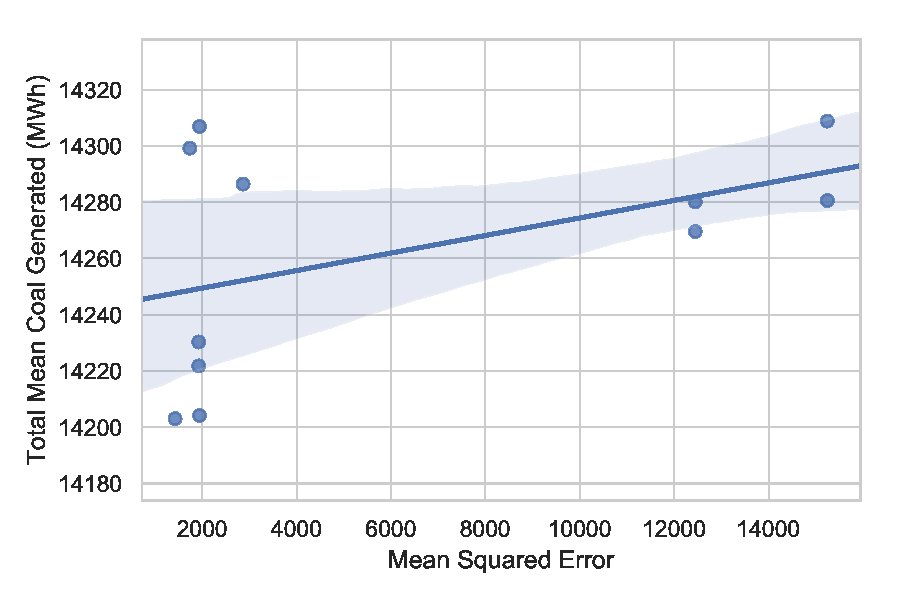
\includegraphics[width=\columnwidth]{Chapter5/figures/market-forecasting/results/elecsim_results/results_2/total_Coal_mean_output.eps}
		\caption{Total Coal.}
		\label{fig:total_Coal_mean_output}
	\end{subfigure}
	\hfil
	%\vskip\baselineskip
	\begin{subfigure}{0.3\textwidth}   
		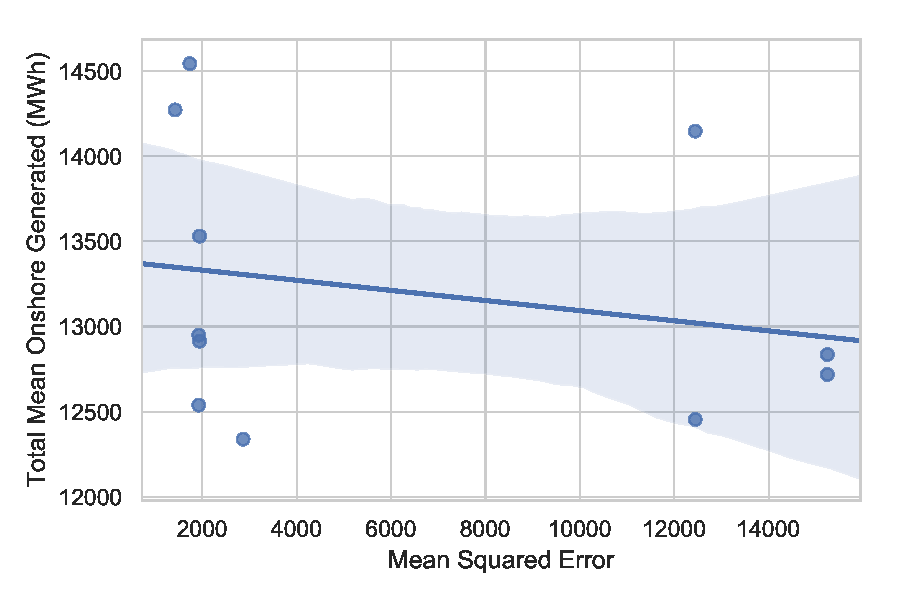
\includegraphics[width=\columnwidth]{Chapter5/figures/market-forecasting/results/elecsim_results/results_2/total_Onshore_mean_output.eps}
		\caption{Total Onshore.}
		\label{fig:total_Onshore_mean_output}
	\end{subfigure}
	%\quad
	\medskip
	\begin{subfigure}{0.3\textwidth}   
		%\centering
		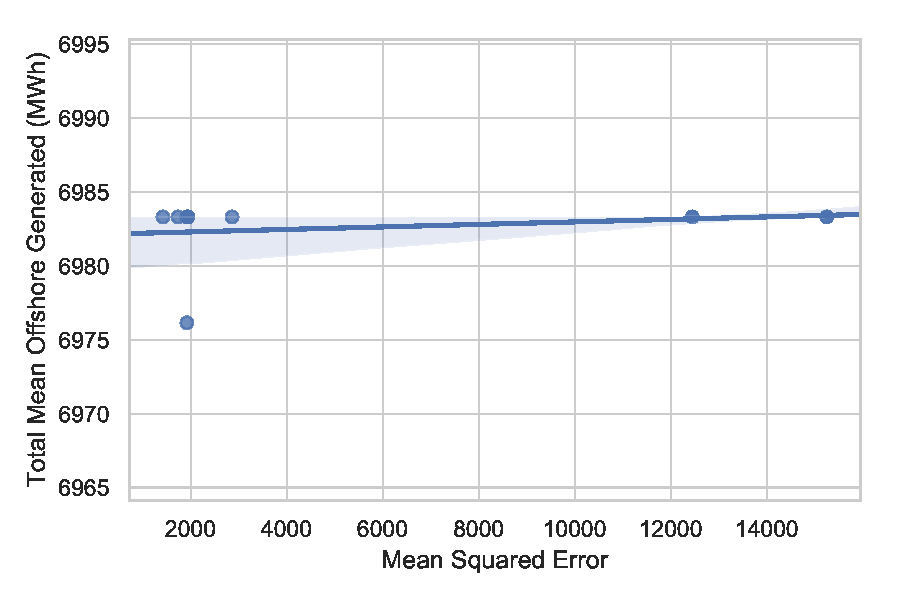
\includegraphics[width=\columnwidth]{Chapter5/figures/market-forecasting/results/elecsim_results/results_2/total_Offshore_mean_output.eps}
		\caption{Total Offshore.}
		\label{fig:total_Offshore_mean_output}
	\end{subfigure}
	\hfil
	\begin{subfigure}{0.3\textwidth}
		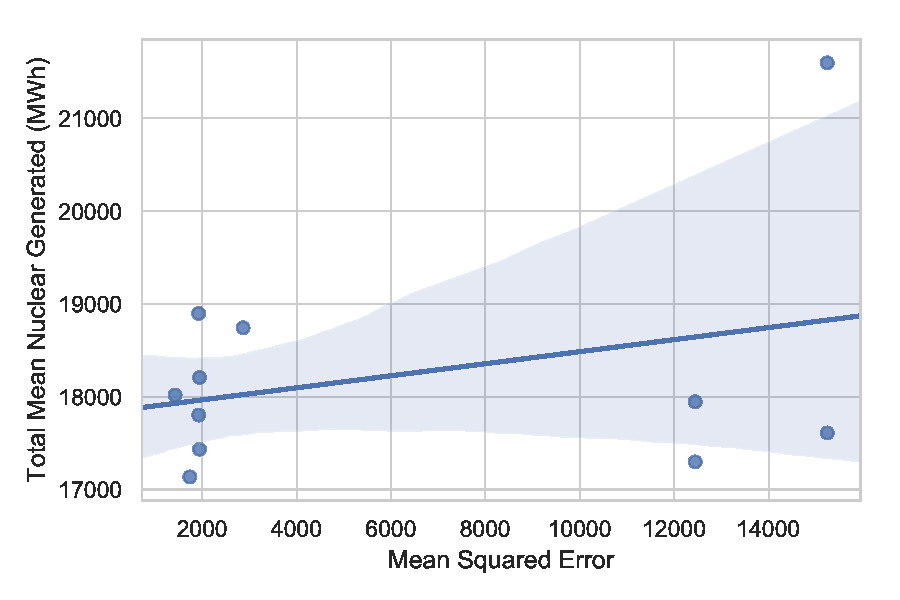
\includegraphics[width=\columnwidth]{Chapter5/figures/market-forecasting/results/elecsim_results/results_2/total_Nuclear_mean_output.eps}
		\caption{Total nuclear.}
		\label{fig:total_nuclear_mean_output}
	\end{subfigure}
	\hfil
	\begin{subfigure}{0.3\textwidth}  
		%\centering
		%\centering
		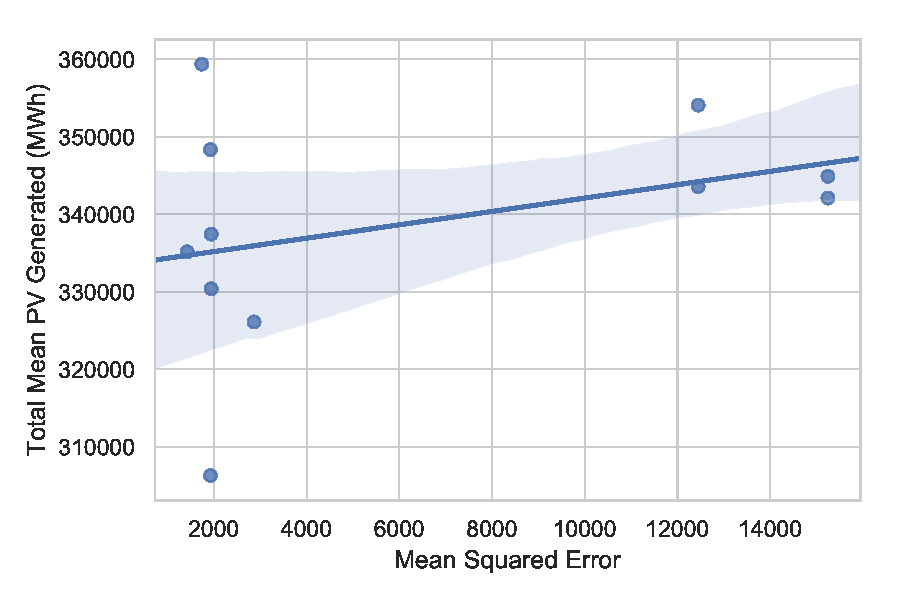
\includegraphics[width=\columnwidth]{Chapter5/figures/market-forecasting/results/elecsim_results/results_2/total_PV_mean_output.eps}
		\caption{Total photovoltaics.}
		\label{fig:total_PV_mean_output}
	\end{subfigure}
	\label{fig:ccgt_coal_onshore_offshore_totals}
	\caption{Total technologies invested in vs. mean absolute error from 2018 to 2035 in ElecSim.}
\end{figure*}




Figure \ref{fig:Carbon_emitted_mean_output} shows an increase in relative mean carbon emitted with mean absolute error of the predictions residuals. The reason for an increase in relative carbon emitted could be due to the increased output of utility of the reciprocal gas engine, coal, and decrease in offshore output. Reciprocal gas engines are peaker plants and, along with coal, can be dispatched. By being dispatched, the errors in predictions of demand can be filled. It is therefore recommended that by improving the demand prediction algorithms, significant gains can be made in reducing carbon emissions.



\begin{figure}
	\centering
	%\vskip\baselineskip
	\begin{subfigure}{0.33\textwidth}   
		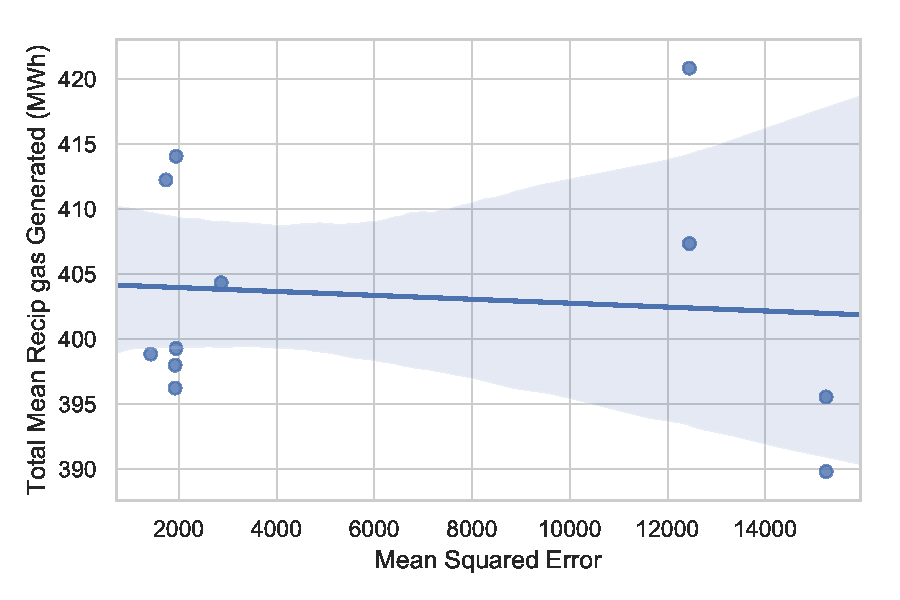
\includegraphics[width=\columnwidth]{Chapter5/figures/market-forecasting/results/elecsim_results/results_2/total_Recip_gas_mean_output.eps}
		\caption{Total Reciprocal gas engine.}
		\label{fig:total_Recip_gas_mean_output.eps}
	\end{subfigure}
	%\quad
	%\medskip
	\hfil
	\begin{subfigure}{0.33\textwidth}   
		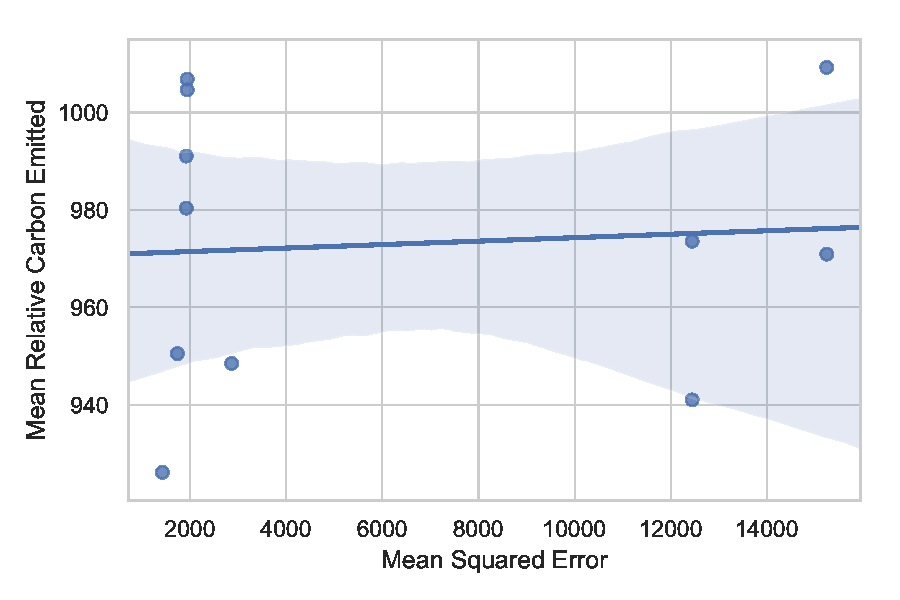
\includegraphics[width=\columnwidth]{Chapter5/figures/market-forecasting/results/elecsim_results/results_2/Carbon_emitted_mean_output.eps}
		\caption{Mean carbon emitted.}
		\label{fig:Carbon_emitted_mean_output}
	\end{subfigure}
	\label{fig:nuclear_pv_carbon_totals}
	\caption{a) Investments in reciprocal gas engine technologies vs. mean absolute error from 2018 to 2035 in ElecSim and d) mean carbon emissions between 2018 and 2035.}
\end{figure}






%\begin{figure}
%\centering
%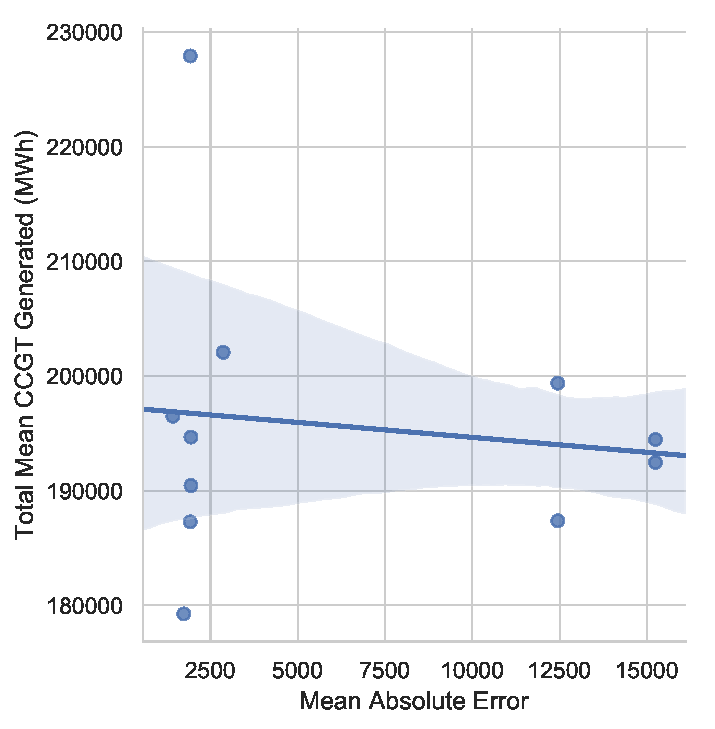
\includegraphics[width=\columnwidth]{Chapter5/figures/market-forecasting/results/elecsim_results/total_CCGT_mean_output.eps}
%\caption{Total CCGT invested in vs. mean absolute error from 2018 to 2035 in ElecSim.}
%\label{fig:total_CCGT_mean_output}
%\end{figure}
%
%
%\begin{figure}
%\centering
%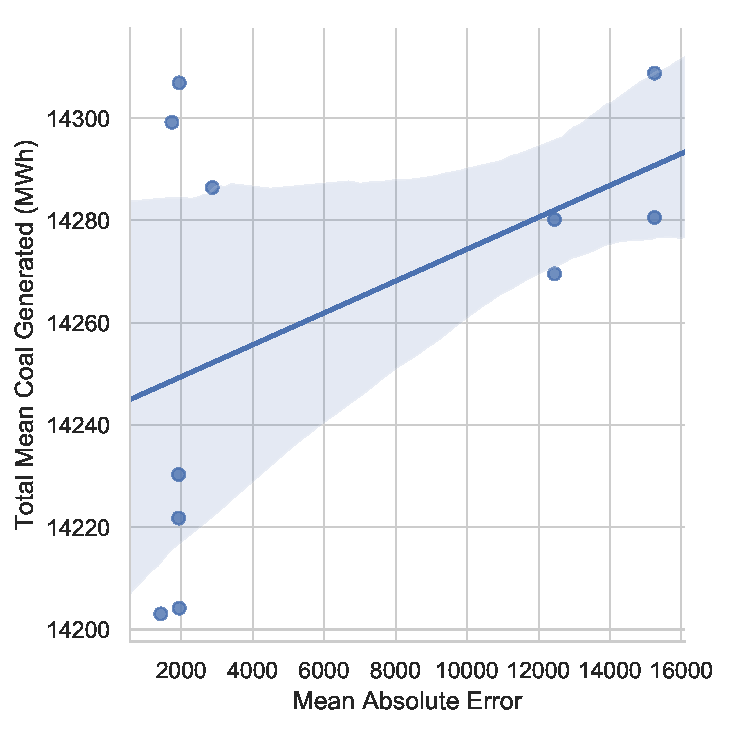
\includegraphics[width=\columnwidth]{Chapter5/figures/market-forecasting/results/elecsim_results/total_Coal_mean_output.eps}
%\caption{Total Coal invested in vs. mean absolute error from 2018 to 2035 in ElecSim.}
%\label{fig:total_Coal_mean_output}
%\end{figure}
%
%
%
%\begin{figure}
%\centering
%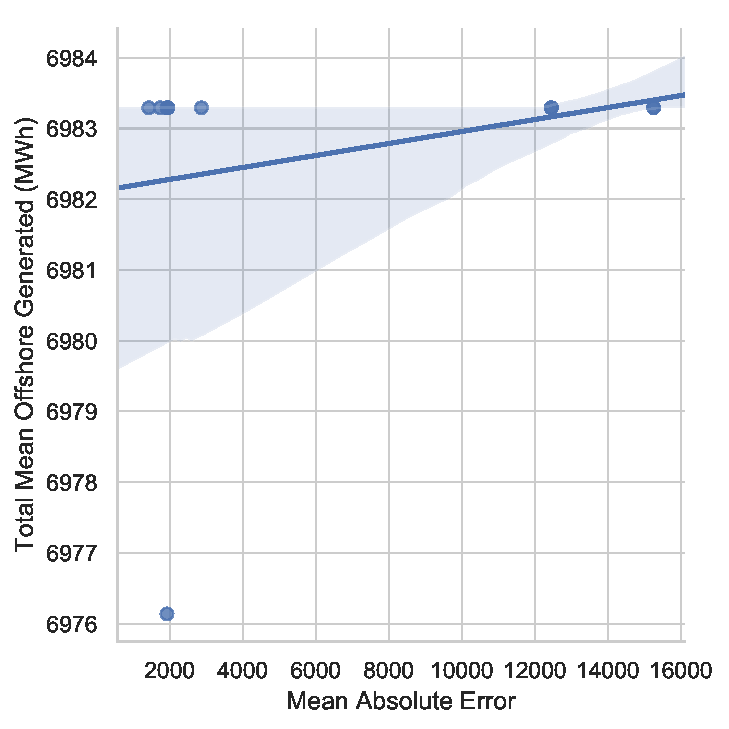
\includegraphics[width=\columnwidth]{Chapter5/figures/market-forecasting/results/elecsim_results/total_Offshore_mean_output.eps}
%\caption{Total Offshore invested in vs. mean absolute error from 2018 to 2035 in ElecSim.}
%\label{fig:total_Offshore_mean_output}
%\end{figure}





%\begin{figure}
%\centering
%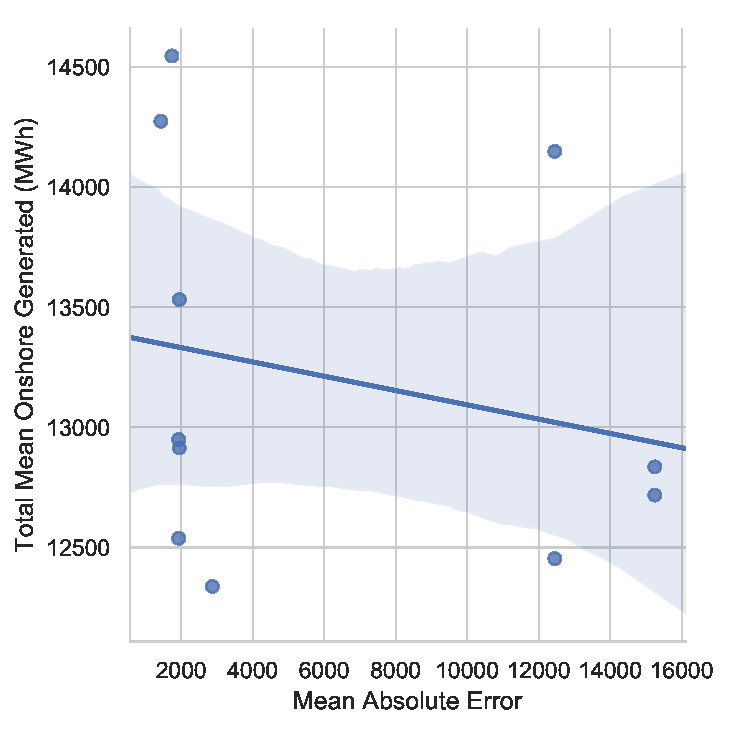
\includegraphics[width=\columnwidth]{Chapter5/figures/market-forecasting/results/elecsim_results/total_Onshore_mean_output.eps}
%\caption{Total Onshore invested in vs. mean absolute error from 2018 to 2035 in ElecSim.}
%\label{fig:total_Onshore_mean_output}
%\end{figure}


%\begin{figure}
%\centering
%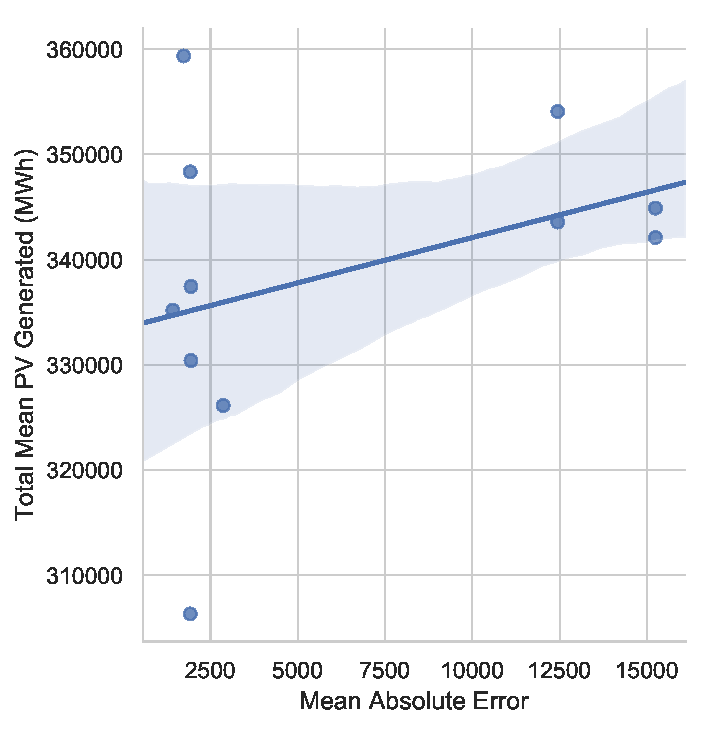
\includegraphics[width=\columnwidth]{Chapter5/figures/market-forecasting/results/elecsim_results/total_PV_mean_output.eps}
%\caption{Total photovoltaics invested in vs. mean absolute error from 2018 to 2035 in ElecSim.}
%\label{fig:total_PV_mean_output}
%\end{figure}

%\begin{figure}
%\centering
%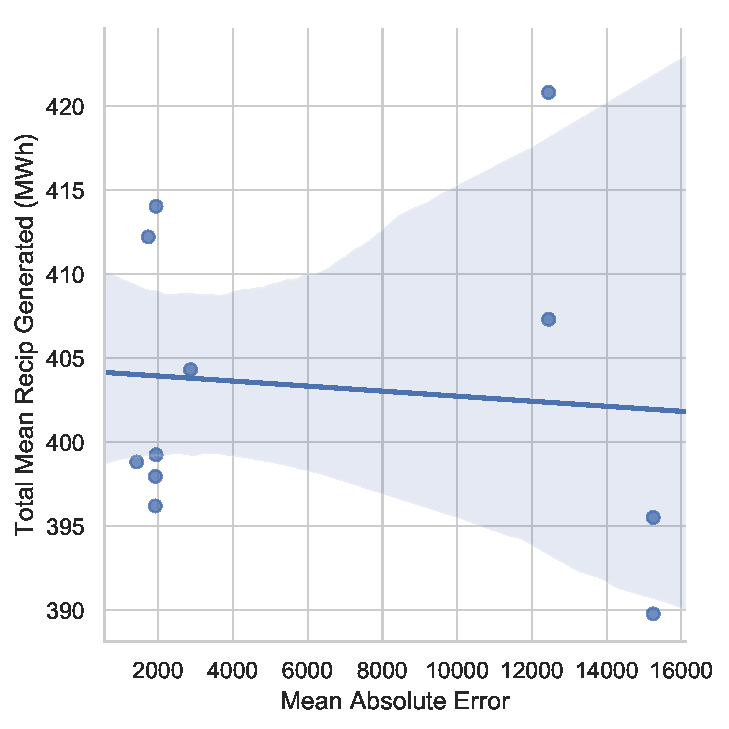
\includegraphics[width=\columnwidth]{Chapter5/figures/market-forecasting/results/elecsim_results/total_Recip_gas_mean_output.eps}
%\caption{Total Reciprocal gas engine invested in vs. mean absolute error from 2018 to 2035 in ElecSim.}
%\label{fig:total_Recip_gas_mean_output.eps}
%\end{figure}


%- Include residuals and MAE,MAPE,MASE etc\\


\subsection{Discussion}
\label{sec:discussion}

%- Discuss the impact of this on the electricity market and the global economy. Make suggestions.

From our results, it can be seen that different algorithms yield differing prediction accuracies. Online models can result in a decrease in 30\% of prediction error on the best offline models. We calculated this by comparing the MAE for Extra Trees to the MAE for the Box-Cox regressor. We, therefore, recommend the use of online machine learning for predicting electricity demand in a day-ahead market.

Similar to our assumptions, the online learning algorithms were able to outperform the offline models. This is due to the non-stationary nature of the data. An online method is able to use the most up-to-date knowledge of the complex system of energy demand. For instance, a certain year may have a particularly warm winter when compared to previous years, reducing the amount of electricity used for heating.

However, contrary to our assumptions, the online linear regression techniques outperformed the online machine learning techniques. This may be due to their simpler nature and ability to learn from a smaller subset of new data as opposed to relying on a large historic subset. For the offline models, the best performing algorithms were the decision tree approaches such as extra trees and random forests. This is a similar outcome to our previous work, which showed that the best performing method for demand forecasting were random forests \cite{Kell2018}. Contrary to our assumptions, however, the lasso and ridge regression outperformed the machine learning techniques support vector regression and multilayer perceptron. This may be due to the ability of feature selection by lasso and ridge regression, which only uses the most important features.

To the best of our knowledge, more work has been done using offline learning to predict electricity demand. This may be due to the additional complexity of running online algorithms, and a smaller number of available models to run in an online fashion.

In terms of computing power, finding the optimal input parameters, hyperparameters and models to use can be a large undertaking. This is due to the exponential growth of the number of choices that can be made. This can be an issue where accuracy is of importance, especially when the data changes over time, meaning it may be necessary to retest previous results. However, due to the financial and sustainability implications, we believe the trade-off between compute time and accuracy is balanced towards compute time. There are also large implications if the model were to break at a certain point in time. We, therefore, recommend the reliance on multiple well-performing models, as opposed to solely the best performing model at any one time. 

For training time and prediction time, there is often a trade-off between training and predicting. For instance, the k-nearest neighbours is fast to train, but slow to sample from. Therefore stakeholders must make a decision based upon accuracy, speed of training and sampling. 

Additionally, the impact on the broader electricity market has been shown to be significant. Principally, the investment behaviours of generation companies change as well as the dispatched electricity mix. The relative mean carbon emitted over this time period increases, due to an increase in the utilization of coal and reciprocal gas engines, at the expense of offshore wind.


\subsection{Conclusion}
\label{sec:conclusion}

In this work, we evaluated 16 different machine learning and statistical models to predict electricity demand in the UK for the day-ahead market. Specifically, we used both online and offline algorithms to predict electricity demand 24 hours ahead. We compared the ability for the offline models: lasso regression, random forests, support vector regression, for both online and offline learning: linear regression, multilayer perceptron and for just online learning: the Box-Cox transformation and the passive aggressive regressor, amongst others. The Box-Cox, as well as the passive aggressive regressors, were used as online learning algorithms, the multilayer perceptron and linear regression were used as both, whereas the rest were used as offline learning algorithms.

We measured the errors and compared these to each model as well as the national grid reserve. We found that through the use of an online learning approach, we were able to significantly reduce error by 30\% on the best offline algorithm.  We were also able to reduce our errors to significantly below the national grid's mean and maximum tendered reserve, thus significantly reducing the chances of blackouts.

In addition to this, we took these errors, or residuals, and perturbed the electricity market of the agent-based model ElecSim. This enabled us to see the impact of different error distributions on the long-term electricity market, both in terms of investment and in terms of the electricity mix.

We observed that with an increase in prediction errors, we get a higher proportion of electricity generated by coal, offshore, nuclear, reciprocal gas engines and photovoltaics. This could be due to the fact that more peaker and dispatchable plants are required to fill in for unexpected demand. In addition, a higher proportion of intermittent renewable energy sources leads to a higher use of peaker power plants to fill in the gaps of intermittency of wind and solar irradiance. However, by reducing the mean absolute error, we are able to significantly reduce the amount of reciprocal gas engines and coal usage.

In future work, we would like to trial a different selection of algorithms and statistical models and trial different inputs to the models, for instance, by providing the model with two months worth of historical data as dependent variables. Additionally, we would like to see the impact of predicting wind speed and solar irradiance to see how these impact the overall investment patterns and electricity mix. 



%\section{Conclusion}
%\label{forecast:sec:conclusion}














%\section{Full paper}
%
%\begin{abstract}
%	
%	Short term load forecasting is utilised in real-time scheduling of electricity as well as load-frequency control. This paper aims to improve the accuracy of load-forecasting by using different machine learning techniques to predict 30 minutes ahead using smart meter data. We utilised a \textit{k}-means clustering algorithm to cluster similar individual consumers and fit distinct models for each cluster. Public holidays were taken into consideration to account for changing customer behaviour on these days. We implemented random forests, neural networks, long short-term memory neural networks and support vector regression models and compared their accuracy using mean absolute percentage error (MAPE). The model with the highest accuracy was a random forest, and we found that clustering similar consumers and aggregating their predictions outperformed a single model in each case.
%\end{abstract}









%\section{Note paper}
%
%\section{Introduction}
%
%The energy markets have undergone significant changes in recent years. The liberalisation of the energy industry, technological advancements and policy changes have had numerous effects \cite{Viegas2016}. These include a rise in both competition and data \cite{sioshansi_2009, Clastres2011}. %, as well as a requirement to integrate large amounts of intermittent renewable resources \cite{Haben2013a,Kamgarpour2013,Curves2014}.
%
%Accurate load forecasting is essential for control and planning of electricity generation in electrical grids as supply must meet demand \cite{Lu1993}. Accurate estimates of demand are required so that the correct amount of electricity is purchased on the wholesale market \cite{Dillon1991}. Failure to accurately forecast electricity demand can lead to financial loss or system-wide blackouts \cite{Hines2008}.
%
%The introduction of smart meters in many countries (USA, Europe and South Korea) has led to an influx of high granularity electricity consumption data that can be used for load forecasting \cite{Depuru2011a}. 800 million smart meters are projected to be installed worldwide by 2020 \cite{Telefonica2014}. 
%
%This paper explores short-term load-forecasting at an interval of 30 minutes ahead and clusters similar users based on their electricity consumption. A variety of different forecasting techniques were evaluated such as Random Forests \cite{TinKamHo}, Long Short-Term Memory Neural Networks (LSTM) \cite{lstm}, Artificial Neural Networks \cite{book:984557} (ANN) and Support Vector Regression (SVR) \cite{Drucker1997}. 
%
%Random Forests are an ensemble-based learning method for classification and regression, and are made up of many decision trees. LSTMs are recurrent Neural Networks which remember values over arbitrary time intervals. Multilayer Perceptrons are a popular type of neural network which consist of a minimum of three layers and can be used to make non-linear predictions. \acrshort{svr}s are supervised learning models which analyse data for regression analysis.
%
%To improve forecasting results, \textit{k}-means clustering of smart meter data was evaluated. An average 24-hour electricity load profile per customer was calculated, and the result used for clustering. The clustered sub-system is then aggregated and separate models trained on these aggregates. The yearly, weekly and daily periodicity of electricity load is accounted for by feature vectors. Once forecasts for each cluster are made using the individual models, the results are aggregated for the final predictions. These predictions are compared to the actual results and the accuracy measured using mean absolute percentage error (MAPE) and mean absolute scaled error (MASE).
%
%This paper provides researchers and utilities with methods to maximise forecasting accuracy through the selection of machine learning and clustering algorithms.
%
%This paper is structured as follows. In Section 2 we explore related work of load forecasting. The experiments and their evaluation are discussed in Section 3. The results are discussed in Section 4. In Section 5 we conclude and consider future directions for this work.
%
%\section{Related Work}
%
%The forecasting of aggregated and clustered electricity demand has been the focus of a considerable amount of research in recent years. The research can generally be classified into two classes, Artificial Intelligence (AI) techniques \cite{Kim2000, Tiong2008,Quilumba2014} and classical time series approaches \cite{Nazarko2005ARIMAApproach,Huang2003,Nguyen2017}. For the purposes of our paper we have reviewed artificial intelligence techniques. Please refer to appendix \ref{appendix:time_series} to explore the literature related to classical time series approaches.
%
%Singh \textit{et al.} produced a review of load forecasting techniques and methodologies and reported that hybrid methods, which combine two or more different techniques, are gaining traction, as well as soft computing approaches (AI) such as genetic algorithms \cite{Singh2012}.
%
%\subsection{Artificial Intelligence Techniques}
%
%Dillon \textit{et al.} presented a Neural Network for short-term load forecasting. Their Neural Network consisted of three-layers and used adaptive learning for training \cite{Dillon1991}. They proposed the use of weather information to augment their electricity load data. They found better results with the Adaptive Neural Network than with a linear model, or Non-Adaptive Neural Network. In contrast to Dillon our paper focuses on a Non-Adaptive Neural Network and does not take into account weather information.
%
%Chen \textit{et al.} used an Artificial Neural Network to predict electricity demand of three substations in Taiwan. They integrated temperature data into the model, and showed a higher degree of accuracy when forecasting demand in residential and commercial substations as opposed to industrial. This was due to the ability to model the high usage of air-conditioners in residential and commercial substations using temperature data \cite{Chen1996}. In contrast to the work by Chen \textit{et al.}, we focus on client-side prediction using smart meter data. We were, therefore, able to cluster the data based on load profile, as opposed to grouping based on geographical location.
%
%
%\subsection{Clustering}
%
%Multiple techniques have been proposed for the clustering of electricity load data prior to forecasting. Shu \textit{et al.} and Nagi \textit{et al.} propose a hybrid approach in which self-organizing maps are used to cluster the data, and Support Vector Regression is used for prediction \cite{Shu2006, Tiong2008}. This technique proved robust for different data types. Shu showed that this hybrid approach out-performed a single SVR technique, whilst Nagi showed superior results to a traditional ANN system. In contrast to both Nagi \textit{et al.} and Shu \textit{et al.} our paper utilises \textit{k}-means as the clustering algorithm.
%
%Wijaya \textit{et al.} demonstrated that implementing  a certain number of clusters improved load-forecasting accuracy \cite{Wijaya2010}. However, a study by Ili\'c \textit{et al.}, showed that increasing the number of clusters did not improve accuracy \cite{Ilic2013}.
%
%\section{Methodology}
%
%The work in this paper was run on a MacBook Pro with a quad-core 3.1GHz Intel Core i7 processor with 16 GB 1867 MHz DDR3 of RAM and a 500GB solid state drive (SSD).
%
%\subsection{Data Collection}
%
%Smart meter data obtained from the Irish Social Science Data Archive (ISSDA) was used in this study \cite{cer_2012}. The Commission for Energy Regulation released a public dataset of anonymised smart meter data from the "\textit{Electricity Smart Metering Customer Behaviour Trials}" \cite{setis}. This dataset is made up of over 5000 Irish homes and businesses and is sampled at 30-minute intervals.
%
%The data was recorded between the 14th July 2009 and 31st December 2010. For the purposes of cross-validation this data was split into a training, validation, and testing set. The training set consisted of the first 9 months of data and used to train the models, the validation set consisted of the following 2 months of data and used to tune the hyperparameters, and the test set included the remaining 6 months and used for measuring error. These splits were chosen to balance the training data with the test data and give the models a chance to learn the periodicity inherent in a one year period. Due to the long training times for these algorithms, we worked with a sample of 709 individual Irish homes. However, due to the infrequent requirement to train these models, we believe our technique would be suited for the real life application.
%
%Figure \ref{fig:similar_customers} displays four residential customer daily load profiles. It can be seen that whilst Customer 1 and Customer 2 have similar load profiles, Customer 3 and Customer 4 have significantly different load profiles.  This demonstrates that, whilst electricity consumption changes per-person, it is possible to cluster similar customers by their load profiles.
%\begin{figure}[b]
%	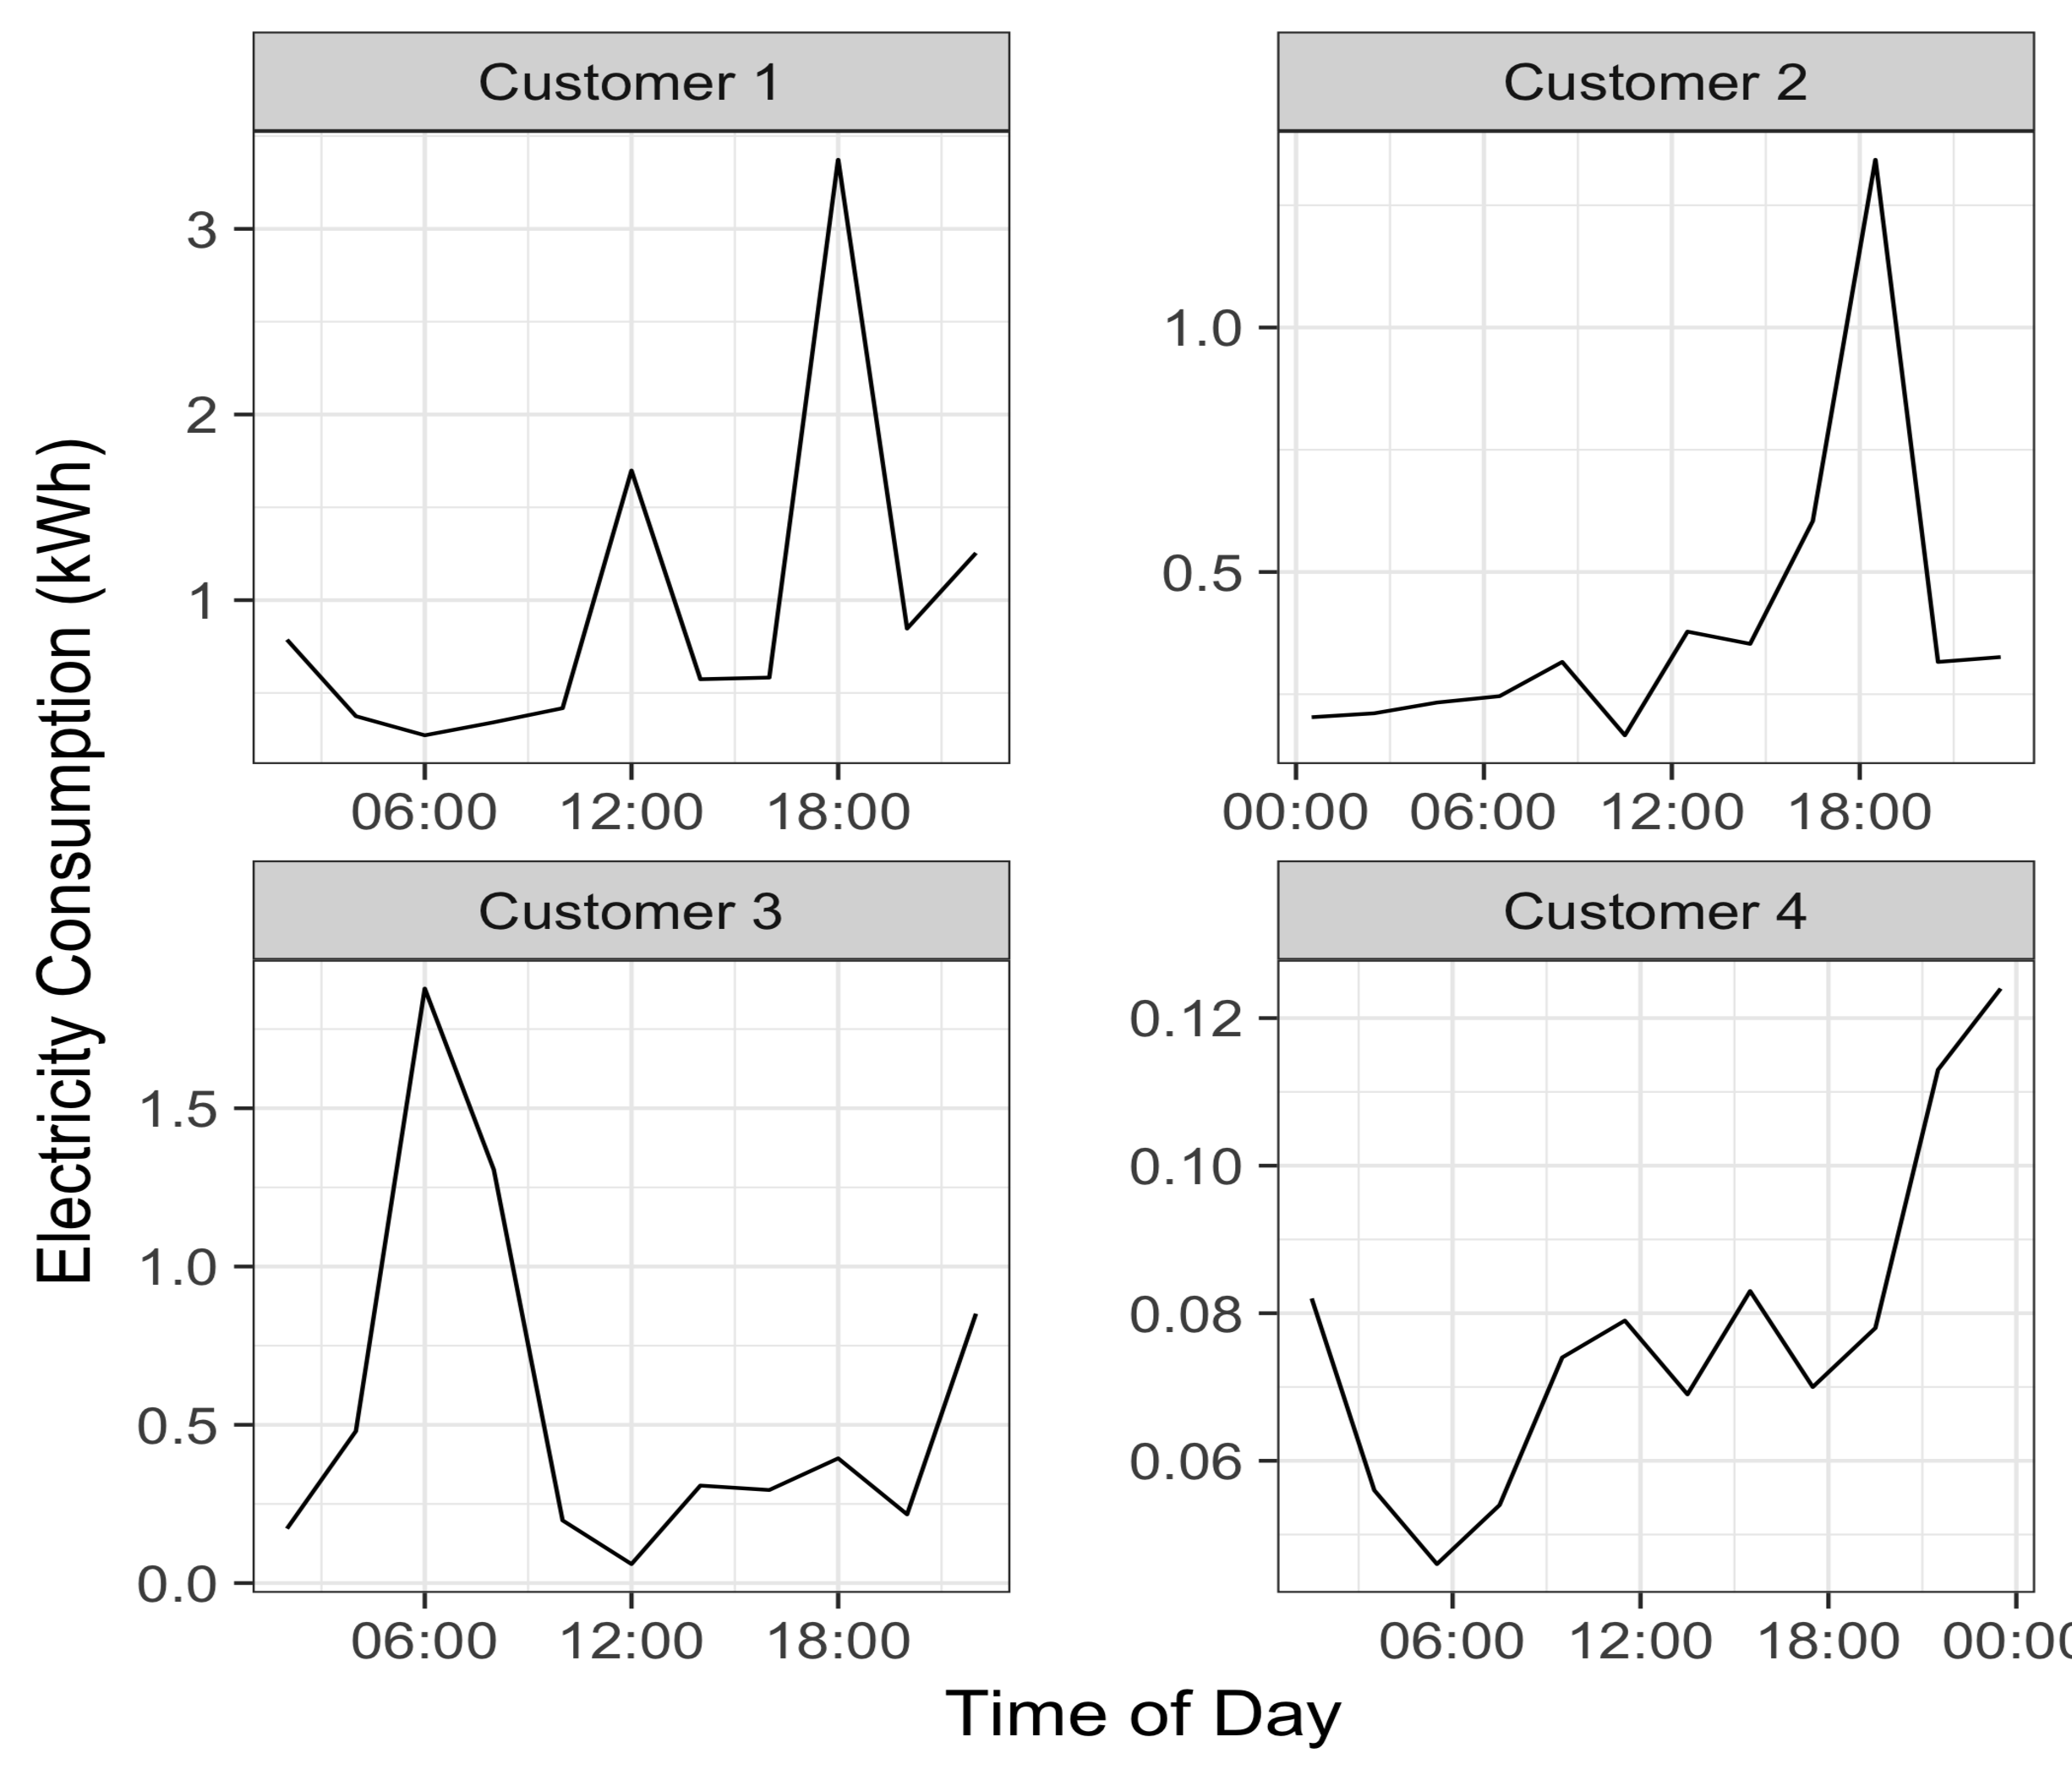
\includegraphics[width=0.8\textwidth]{Chapter5/figures/short-term-forecasting/Webp_net-resizeimage.png}
%	\caption{Figure showing daily load profiles for four different customers on the 22nd July 2009.}
%	\label{fig:similar_customers}
%\end{figure}
%\subsection{Clustering}
%
%We propose that clustering similar customer load profiles and aggregating each cluster's electricity consumption improves the accuracy of the models. This is due to the fact that aggregated clustered loads decrease the stochasticity of the demand of the system, and therefore increase the predictive ability of the models.
%
%The Euclidean distance and wavelet metrics were evaluated using hierarchical clustering~\cite{BIMJ:BIMJ4710240520}. However, \textit{k}-means demonstrated to be the most robust and best-performing algorithm, and thus was chosen for use in this paper \cite{Forgy65}.
%
%To cluster the data, each user's nine month electricity consumption in the training set was reduced to a single averaged 24 hour load profile (48 data points per customer). This was achieved by taking the average electricity consumed for each half hourly point of the day (eg. taking the mean of every 12-12:30pm point in the training set). We did not take into account the difference between weekend and weekdays for clustering. The data was then scaled so that different sized households, but with similar usage profiles were clustered together.
%
%To select the optimum number of clusters (\textit{k}) the test set was used for cross-validation. This allowed us to compare the results of each of the models and select \textit{k} with the highest accuracy exhibited by mean absolute percentage error (MAPE) and mean absolute scaled error (MASE). In this paper \textit{k} was varied between 1 and 7, which was chosen due to the fact that the error did not vary greatly past seven clusters. Multiple models were fit per cluster and used to predict the testing data.
%
%To overcome local minima the \textit{k}-means algorithm was run 1000 times and the most accurate partition chosen \cite{Jain2010}.
%
%\subsection{Aggregating Demand}
%
%Once each customer is assigned to their respective cluster, the total electricity consumed by each cluster is calculated. This is achieved by summing the electricity consumed at every time interval per cluster. This creates a partial system load. A model is trained on each of the different partial system loads, and the resultant forecasts are aggregated to generate the total load forecast. This forecast is then evaluated by calculating the MAPE and MASE for each model. 
%
%\subsection{Feature Selection}
%
%\subsubsection{Calendar Attributes}
%
%Due to the daily, weekly and annual periodicity of the electricity consumption, daily calendar attributes were deemed important to accurately model the problem. The calendar attributes included are: hour of the day, day of the month, day of the week, month, and public holidays.
%
%Public holidays were used as features for the model due to the change in electricity consumption exhibited on these days.
%
%We evaluate the increase in performance due to the modelling of calendar attributes in the results section.
%
%\subsubsection{Time Series Data}
%
%The time-series element was modelled using lagged data inputs. This was achieved using the previous 3 hours, the equivalent 3 hours from the previous day, and the equivalent 3 hours from the previous week.
%
%Long Short-Term Memory neural networks remember values over arbitrary time intervals. And thus can remember short-term memory over a long period of time, for this reason, 5 lagged inputs of the previous two and a half hours were used as features to the Long Short-Term Memory network.
%
%\subsubsection{Data Representation}
%
%Numerical representations were used for the lagged data input. A single binary was used for public holidays. One hot encoding is a method which allows categorical variables to be distinguished from ordinal data. One hot encoding was used to encode day of the week and month of the year. Table \ref{appendix:feature} displays the input data for SVR, Neural Network and Random Forest. 
%
%
%
%\begin{table}
%	\label{appendix:feature}
%	\begin{tabular}{p{1cm}p{3cm}p{8cm}}
%		\toprule
%		Input & Variable      & Detail description \\
%		\midrule
%		1     & Hour          & Single numeric input representing hour of the day                                                                                              \\
%		2     & Day of month  & Single numeric input representing day of the month                                                                                             \\
%		3-9   & Day of week   & Seven binary digits representing calendar information regarding day of the week                                                                                            \\
%		10-21 & Month         & Twelve binary digits representing calendar information regarding month                                                                                         \\
%		22-42 & Lagged inputs & Twenty one numeric inputs representing lagged inputs of previous 3 hours, previous 3 hours of previous day including hour to be predicted, and previous 3 hours of previous week including hour to be predicted \\
%		43    & Holiday       & Single binary digit representing whether the day was a public holiday  \\     \bottomrule                                                           
%	\end{tabular}
%	\caption{List of Input Data for Models}
%\end{table}
%
%\subsection{Experiments}
%
%This section explores the experiments made to design the models. Cross-validation was used on the validation set of each of the models to tune the hyperparameters. Each of the models were then created five times per cluster to explore the variance of the results.
%
%\subsubsection{Support Vector Regression}
%
%The validation set was used to tune the hyperparameters and select the kernel of the SVR model.
%
%The kernels compared were polynomial, radial basis function (RBF) and the linear kernel \cite{Chang2010, theodoridis2009pattern}. They were chosen due to their popularity, support and speed of computation.
%
%The parameter values are shown in Table \ref{tab:kernel}. The linear kernel produced the best results, and therefore chosen as the final model.
%\begin{table}
%\centering
%	\label{tab:kernel}
%	\begin{tabular}{ccl}
%		\toprule
%		Kernel Type& Kernel Parameters & RMSE\\
%		\midrule
%		Linear & No values & 0.02102779\\
%		RBF & C=2, $\gamma=0.016$ & 0.02444950\\
%		Polynomial & C=2, $d=2, r=2$ & 0.03145719 \\
%		\bottomrule
%	\end{tabular}
%\caption{Prediction Accuracy Based on Type of Kernel}
%\end{table}
%\subsubsection{Random Forest}
%The number of variables sampled as candidates at each split was tuned using the validation set.
%
%The optimum number for this was 23. It is proposed that the value 23 was found to be optimum due to the 21 lagged inputs, which are crucial to learn the underlying nature of the time series.
%
%
%\subsubsection{Artificial Neural Network}
%
%The first step when creating an Artificial Neural Network is to design the architecture. In our case, the number of input neurons is set to 43 (see Table \ref{appendix:feature}). Only one output neuron is required, due to the fact that we are only forecasting one step (30 minutes) ahead.
%
%To design the number of hidden layers the Levenberg-Marquardt technique was used. An optimal architecture with three hidden layers was obtained. The first layer contained two neurons, the second contained five, and the third contained four.
%
%\subsubsection{LSTM}
%
%The Levenberg-Marquardt techniques was once again used to select number of layers and number of memory units. Using this technique, the optimum number of layers was found to be 2 with 50 memory units each.
%
%\section{Results}
%\begin{figure}
%	\includegraphics[width=0.8\textwidth]{Chapter5/figures/short-term-forecasting/results.png}
%	\caption{Comparison of accuracy of models forecasting electricity with varying number of clusters.}
%	\label{fig:results}
%\end{figure}
%To determine the optimal number of clusters a range of values for $k$ were explored, thus, $k$ was varied between one and seven. 28 forecasting models were therefore constructed per type of model. The models were fit five times to explore the variation in the output. The model accuracy was evaluated using both MAPE and MASE.
%
%The results are shown in figure \ref{fig:results}. These show that clustering similar users improves accuracy. The optimum value for \textit{k} for every model was shown to be four. After this, the accuracy diminishes slightly. The error bars shown in Figure \ref{fig:results} display a slight variance in MAPE for \acrshort{svr}s, ANNs and Random Forests. However, the MAPE of the LSTMs seem to vary by up to 11\%. 
%
%The MASE metric also demonstrated that four clusters were optimal for SVR, Neural Networks and Random Forests.
%
%\begin{figure}
%	\centering
%	\includegraphics[width=0.8\textwidth]{Chapter5/figures/short-term-forecasting/actual_vs_predicted_enlarged.png}
%	\caption{Real electricity consumption versus predicted electricity consumption between June 16th and June 18th 2010.}
%	\label{fig:act_vs_pred}
%\end{figure}
%
%The impact of using calendar attributes improves prediction accuracy by 6\% for neural networks, 4\% for Random Forests and 1\% for SVR. For these results please see figure \ref{appendix:calendar_attr} in appendix \ref{appendix:results}.
%
%It is proposed that the optimum value for \textit{k} cluster centres was four due to the distinct patterns observed in each of the clusters. At $k=5$ one of the distinct clusters is split, and leads to an increase in stochasticity. At $k=3$ the stochasticity is also increased by the aggregation of load profiles which are dissimilar. % To see a breakdown of the average clusters please refer to figure \ref{appendix:clustercentre} in appendix \ref{appendix:results}.
%
%However, the optimum number of clusters will vary for different datasets. Differing geographies may display varying usage characteristics due to culture, weather or social norms.
%
%The results demonstrate that SVR, Random Forests and the ANN have similar accuracy, and adequately predict electricity consumption. The LSTM shows a similar pattern in increasing accuracy with number of clusters, but performs worse than the other models. The Random Forest seems to outperform each of the other models. This may be due to the internal operation of the Random Forest which undertakes its own cross-validation using out-of-bag samples. 
%
%Figure \ref{fig:act_vs_pred} displays actual electricity consumption versus predicted results. It shows that the LSTM model predicts a similar value in the next time step as the previous time step, which would explain its inferior results to the other models.  
%
%The training times were tested by timing how long the models took to fit for four clusters. The Support Vector Regression took less time than all of the other methods, whereas the LSTM took the longest. The Support Vector Regression model required 3 minutes and 18 seconds to run. The Random Forest required 14 minutes and 58 seconds. The Artificial Neural Network required 17 minutes and 48 seconds, whilst the LSTM took 21 minutes 11 seconds to run.
%
%The time to make a single prediction was recorded at sub microseconds and therefore deemed negligible for our use-case.
%
%\section{Conclusion}
%
%The availability of data produced by smart meters enables network operators to gain greater insights into their customer behaviour and electricity usage. We demonstrated that implementing the \textit{k}-means clustering algorithm to group similar customers improved the accuracy of the models tested. Distinct models were trained for each cluster and the individual forecasts aggregated for the total aggregated forecast. It was found that Random Forests outperformed all other models at each level of clustering. The optimum number of clusters was found to be four. Whilst the dataset used focused on residential data it is expected that applying a similar clustering technique on commercial properties would have a similar effect.
%
%It is considered that monthly retraining of the models would be required to ensure continued accuracy. However, this is not expected to be a problem due to the short time time required for model training. Once trained, the prediction times are negligible.
%
%In future work, we will look into the features that best aid in the forecasting of electricity consumption, try a wider variety of models in an ensemble manner and try different clustering techniques such as self-organizing maps (SOM) to obtain better accuracy results. We will also compare a greater variety of forecasting metrics.
%
%% To utilize more of the data and increase the number of models trained these results could be run in parallel in future.






%%%%%%%%%%%%%%%%%%%%%%%%%%%%%%%%%%%%%%%%%%%%%%%%
%%%%%%%%%%%%%%%%%%%%%%%%      Paper 2    %%%%%%%%%%%%%%%%
%%%%%%%%%%%%%%%%%%%%%%%%%%%%%%%%%%%%%%%%%%%%%%%%	








%\section{The impact of online machine-learning methods on long-term investment decisions and generator utilization in electricity markets}


%\begin{abstract}
%
%% Background
%
%Electricity supply must be matched with demand at all times. This helps reduce the chances of problems with load frequency control and the chances of electricity blackouts. To gain a better understanding of the load that is likely to be required over the next 24 hours, estimations under uncertainty are needed. This is especially difficult in a decentralized electricity market with many micro-producers who are not under central control. 
%
%% Methodology
%
%In this paper, we investigate the impact of 11 offline learning and five online learning algorithms to predict the electricity demand profile over the next 24 hours. We achieve this through integration within the long-term agent-based model, ElecSim. These algorithms include multilayer perceptron neural networks, support vector regression and linear regression. By predicting the electricity demand profile over the next 24 hours, we can simulate the predictions made for a day-ahead market. Once we have made these predictions, we sample from the residual distributions and perturb the electricity market demand using the simulation, ElecSim. This enables us to understand the impact of errors on the long-term dynamics of a decentralized electricity market.
% 
%
%% Results  
%
%Our results show that we are able to reduce the mean absolute error by 30\% using an online algorithm when compared to the best offline model, whilst reducing the required tendered national grid reserve required. Such a reduction allows for a smaller required tendered grid reserve, saving costs and emissions. We also show that large errors in prediction accuracy have a disproportionate error on investments made over a 17-year time frame, as well as electricity mix.
%
%
%\end{abstract}



%
%%%Graphical abstract
%\begin{graphicalabstract}
%\includegraphics{grabs}
%Hello test
%\end{graphicalabstract}
%
%%%Research highlights
%\begin{highlights}
%\item Validating a model
%\item Optimisation
%\item Scenario modelling
%\end{highlights}
%
%Chapter5/figures/
%% \linenumbers

%% main text





